\documentclass[zihao=-4,fontset=windows,twoside]{ctexbook}
\overfullrule=1pt
\usepackage[dvipsnames,svgnames,x11names,table]{xcolor}
\usepackage{cncolours}
\usepackage{pgfornament-han}
\usepackage{tikz}
\usetikzlibrary{calc,shadows,hobby,intersections, decorations.markings, decorations.pathreplacing,spy,arrows,shapes,fadings,trees,mindmap,patterns,shapes.arrows,shapes.symbols,tikzmark,shapes.geometric,graphs, quotes, angles,decorations.pathmorphing,through,shadings,backgrounds,positioning,fit,arrows.meta,shapes.misc,decorations.shapes}
\RequirePackage{pgfplots} %画图 %%页面样式设计核心包 %提供\pgfonlayer命令以及下列图层指令
\pgfplotsset{compat=1.18}
\usepackage{stys/Titlepage}
\usepackage{stys/bottompage}
\usepackage{amssymb,amsfonts}
\usepackage{makeidx}
\usepackage{etoolbox} % 判断函数
\usepackage{paracol}
\usepackage{etoc}
\usepackage{calc}
\usepackage{xkeyval,ifthen}
\usepackage[backgroundcolor=yellow!40!cyan!20,bordercolor=yellow!40!cyan!20,linecolor=DarkCyan]{todonotes}
\usepackage{varwidth}
\usepackage[colorlinks,linkcolor = DarkCyan,		%%修改此处为你想要的颜色
anchorcolor = DarkCyan,	%%修改此处为你想要的颜色
urlcolor = DarkCyan,		%%修改此处为你想要的颜色
citecolor = DarkCyan,		%%修改此处为你想要的颜色
]{hyperref}
\setcounter{tocdepth}{3}
\setcounter{secnumdepth}{3}%增加编号深度
\usepackage{dashrule}
\newlength\outermarginwidth
\setlength\outermarginwidth{2cm}
\newlength\covershift
\setlength\covershift{5cm}
\makeatletter
%%----------------------------------封面信息定义--------------------------------------------------------%%
\newcommand*\bookseries[1]{\def\@bookseries{#1}}
\newcommand*\subtitle[1]{\def\@subtitle{#1}}
\newcommand*\edition[1]{\def\@edition{#1}}
\newcommand*\presslogo[1]{\def\@presslogo{#1}}
\newcommand*\pressname[1]{\def\@pressname{#1}}
\newcommand*\coverimage[1]{\def\@coverimage{#1}}
%%----------------------------------封面信息定义--------------------------------------------------------%%
\makeatother
\usepackage{indentfirst}
\usepackage{physics}
\definecolor{nuanbai}{HTML}{f8f8f8} % F5F5F5
\pagecolor{nuanbai!50}
\usepackage{amsmath}
\usepackage{zhlipsum}
\setmainfont{XITS}
\usepackage[left=2cm,right=2cm,top=.8cm,bottom=3.6cm]{geometry}
\usepackage{xpatch}%修正章节编号
\usepackage[automark]{scrlayer-scrpage}%页面设置宏包,隶属于koma-script文档类
% \setcounter{secnumdepth}{5}%增加编号深度
% \setcounter{tocdepth}{3} %增加目录深度
\usepackage{fontawesome5}
\usepackage{mathrsfs}

\usepackage[most]{tcolorbox}
\tcbuselibrary{breakable, skins,theorems}%TcolorBox Library
\usepackage{tabularx}
\usepackage{lastpage}
\usepackage{ninecolors}
\usepackage{colortbl} %彩色表格
\usepackage{tabularray}
\usepackage{pgfornament}
\usepackage{zhnumber}
\usepackage{dashrule}
\usepackage{adjustbox}
\usepackage{enumitem}
\usepackage{multicol}
\usepackage{amsthm}
\usepackage{bclogo}
\usepackage{ulem}
\RequirePackage{pgfplots} %画图 %%页面样式设计核心包 %提供\pgfonlayer命令以及下列图层指令
\pgfplotsset{compat=1.18}
\usepackage{graphicx}%修正minipage顶部对齐问题

\pgfdeclarelayer{background} %背景%底层
\pgfdeclarelayer{foreground} %上层
\pgfdeclarelayer{top} %顶部
\pgfdeclarelayer{bottom} %底部
\pgfsetlayers{bottom,background,main,foreground,top}
%%%%===============================================================%%%%%

\definecolor{qing}{HTML}{a88462}
\definecolor{xieqing}{HTML}{88ada6}
\definecolor{hex}{RGB}{217,230,232}  %grey
\definecolor{hui}{HTML}{fffbf0}

\newcommand{\triangler}[2][teal]{
\begin{tikzpicture}[remember picture]
\def\x{#2}
\filldraw[#1] (-\x,\x) -- (0,0) --(-\x,-\x)--cycle;
\filldraw[#1] (0,\x) -- (\x,0) -- (0,-\x)--cycle;
\filldraw[#1] (\x,\x) -- (2*\x,0) -- (\x,-\x)--cycle;
\end{tikzpicture}
}
\newcommand{\trianglel}[2][teal]{
\begin{tikzpicture}[remember picture]
\def\x{#2}
\filldraw[#1] (\x,\x) -- (0,0) --(\x,-\x)--cycle;
\filldraw[#1] (0,\x) -- (-\x,0) -- (0,-\x)--cycle;
\filldraw[#1] (-\x,\x) -- (-2*\x,0) -- (-\x,-\x)--cycle;
\end{tikzpicture}
}
\usepackage{lastpage}
% 重置\rightmark与\leftmark名称
\renewcommand{\chaptermark}[1]{\markboth{第{\upshape\thechapter} 章~ #1}{}}
\renewcommand{\sectionmark}[1]{\markright{{\upshape\thesection}\ #1}}

\setlength{\headheight}{50pt}
\newlength\headradii
\setlength\headradii{.16\headheight}
\newcommand{\headstyle}{
    \begin{tikzpicture}[remember picture,overlay]
    \ifodd\value{page}
    \path[fill,gray!40]
    ([xshift=-\headheight,yshift=-.9\headheight]current page.north east) -- ([xshift=-.9\headheight-2cm,yshift=-.9\headheight]current page.north east) coordinate (NW) -- ([xshift=-3pt,yshift=-3.5pt]NW) node[above,text=black] (vline) {\color{black}\tikz\draw[line width=1pt] (0,0)--(0,.3\headheight);}--([xshift=-6pt]NW) -- ([xshift=\headheight,yshift=-.9\headheight]current page.north west)|-([xshift=-\headheight,yshift=-\headheight]current page.north east) --cycle;
    % \node[right,font=\upshape] at (vline) {\thepage\ (\pageref{LastPage})};
    \node[left] at (vline) {\begin{varwidth}{.9\linewidth}\trianglel[gray!50]{.45em}\rightmark\end{varwidth}};
    
    \path[fill,xieqing] ([shift={(-\headheight,-.9\headheight+2*\headradii)}]current page.north east) coordinate (NE) -- ([shift={(-1.5cm,0)}]NE) arc(90:270:\headradii) -- ([shift={(0,-2*\headradii)}]NE)--cycle;
    \fill[xieqing!30] ([shift={(-1.5cm,0)}]NE) coordinate (ul) arc(90:270:\headradii)--++(1cm,0) coordinate (dr) arc(-90:90:\headradii)--cycle;
    \node[font=\bfseries\upshape,text=black](pagenumber) at ($(ul)!0.5!(dr)$) {\thechapter\ 章};
        \else
        \path[fill,gray!40]
        ([xshift=\headheight,yshift=-.9\headheight]current page.north west) -- ([xshift=.9\headheight+2cm,yshift=-.9\headheight]current page.north west) coordinate (NW) -- ([xshift=3pt,yshift=-3.5pt]NW) node[above,text=black] (vline) {\color{black}\tikz\draw[line width=1pt] (0,0)--(0,.3\headheight);}--([xshift=6pt]NW) -- ([xshift=-\headheight,yshift=-.9\headheight]current page.north east)|-([xshift=\headheight,,yshift=-\headheight]current page.north west) --cycle;
    % \node[left,font=\upshape] at (vline) {(\pageref{LastPage})\ \thepage};
    \node[right] at (vline) {\begin{varwidth}{.9\linewidth}\leftmark\triangler[gray!50]{.45em}\end{varwidth}};
    \path[fill,xieqing] ([shift={(\headheight,-.9\headheight+2*\headradii)}]current page.north west) coordinate (Nl) -- ([shift={(1.5cm,0)}]Nl) arc(90:-90:\headradii) -- ([shift={(0,-2*\headradii)}]Nl)--cycle;
    \fill[xieqing!30] ([shift={(1.5cm,0)}]Nl) coordinate (ull) arc(90:-90:\headradii)--++(-1cm,0) coordinate (drr) arc(270:90:\headradii)--cycle;
    \node[font=\bfseries\upshape,text=black](pagenumberr) at ($(ull)!0.5!(drr)$) {\thesection\ 节};
    \fi
    \end{tikzpicture}
}
\newcommand{\pageheadstyle}{%
    \begin{tikzpicture}[remember picture,overlay]
    \coordinate (page head odd) at ([shift={(-\headheight,-.8\headheight)}]current page.north east);
    \coordinate (page head even) at ([shift={(\headheight,-.8\headheight)}]current page.north west);
    \ifodd\value{page}
    \node[single arrow ,fill=hex!50,font=\bfseries\upshape,text=black,minimum height=8mm,left]
    (page head information odd) at (page head odd) {\begin{varwidth}{.85\linewidth}\leftmark\end{varwidth}};
    \else 
    \node[signal ,fill=hex!50,font=\bfseries\upshape,text=black,minimum height=8mm,right]
    (page head information even) at (page head even) {\begin{varwidth}{.85\linewidth}\rightmark\end{varwidth}};
    \fi    
    \end{tikzpicture}
}
\ihead{}
\ohead{}
\setlength{\headheight}{50pt}
\chead{\headstyle}
%%页脚
\ifoot{}
\cfoot{}
\ofoot{\footSt}
\setlength\footheight{50pt}
\newcommand{\footSt}{
    \begin{tikzpicture}[remember picture,overlay]
        \coordinate (page num odd) at ([shift={(\footheight,.9\footheight)}]current page.south west);
        \coordinate (page num even) at ([shift={(-\footheight,.9\footheight)}]current page.south east);
        \ifodd\value{page}
    \node[circle,fill=gray!30,text=black,font=\bfseries\upshape,minimum size=6mm] (page numr) at (page num even) {\thepage};
        \draw[line width=1.5pt] (page numr.west)--([xshift=-.2\linewidth]page numr.west) node[font=\slshape,text=black,left] {\begin{varwidth}{.75\linewidth}\leftmark\end{varwidth}};
        \else 
        \node[circle,fill=gray!30,text=black,font=\bfseries\upshape,minimum size=6mm] (page numl) at (page num odd) {\thepage};
        \draw[line width=1.5pt] (page numl.east)--([xshift=.2\linewidth]page numl.east) node[font=\slshape,text=black,right] {\begin{varwidth}{.75\linewidth}\rightmark\end{varwidth}};
        \fi
    \end{tikzpicture}
}
\usepackage[explicit]{titlesec}
\newtheorem*{solution}{\textbf{解答:~}}
\newtheorem{defi}{\textbf{定义}}[section]
\newtheorem{thm}{\textbf{定理}}[section]
\newtheorem{lem}{\textbf{引理}}[section]
\newtheorem{prop}{\textbf{命题}}[section]
\renewcommand{\proofname}{\textbf{证明.}}
\newtheorem{exam}{\textbf{题}}[chapter]
\newtheorem{cor}{\textbf{推论}}[chapter]
\newtheorem*{remark}{\textbf{评注}}

\colorlet{CyaN}{yellow!40!cyan}
\colorlet{OrangE}{yellow!20!orange}
\colorlet{BluE}{cyan!70!blue}
\colorlet{ReD}{red!20!orange}
\colorlet{GreeN}{yellow!40!green}
\tcolorboxenvironment{thm}{enhanced jigsaw, breakable, enlarge left by=-3.5mm, width=\textwidth+3.5mm, colback=CyaN!10, boxrule=0pt, top=2pt, bottom=2pt, left=2.5mm, borderline west={1.5mm}{0mm}{CyaN}, frame hidden}
\tcolorboxenvironment{defi}{enhanced jigsaw, breakable, enlarge left by=-3.5mm, width=\textwidth+3.5mm, colback=ReD!5, boxrule=0pt, top=2pt, bottom=2pt, left=2.5mm, borderline west={1.5mm}{0mm}{ReD}, frame hidden}
\tcolorboxenvironment{lem}{enhanced jigsaw, breakable, enlarge left by=-3.5mm, width=\textwidth+3.5mm, colback=BluE!5, boxrule=0pt, top=2pt, bottom=2pt, left=2.5mm, borderline west={1.5mm}{0mm}{BluE}, frame hidden}
\tcolorboxenvironment{prop}{enhanced jigsaw, breakable, enlarge left by=-3.5mm, width=\textwidth+3.5mm, colback=OrangE!5, boxrule=0pt, top=2pt, bottom=2pt, left=2.5mm, borderline west={1.5mm}{0mm}{OrangE}, frame hidden}
\tcolorboxenvironment{exam}{enhanced jigsaw, breakable, enlarge left by=-3.5mm, width=\textwidth+3.5mm, colback=GreeN!5, boxrule=0pt, top=2pt, bottom=2pt, left=2.5mm, borderline west={1.5mm}{0mm}{DarkGreen}, frame hidden}
\tcolorboxenvironment{cor}{enhanced jigsaw, breakable, enlarge left by=-3.5mm, width=\textwidth+3.5mm, colback=violet!5, boxrule=0pt, top=2pt, bottom=2pt, left=2.5mm, borderline west={1.5mm}{0mm}{violet}, frame hidden}
\newcommand*{\circled}[1]{\lower.7ex\hbox{\tikz\draw (0pt, 0pt)%
    circle (.5em) node {\makebox[1em][c]{\small #1}};}}
\newcommand{\twicecircle}{\raisebox{.7ex}{
    \begin{tikzpicture}[remember picture,overlay]
        \draw[line width=0.6pt,black!60] (0,0) circle (3pt);
        \fill[black]  (0,0) circle (1.6pt) ;
    \end{tikzpicture}}
}
\newcommand{\exercise}[2][\bcicosaedre]{\bigskip
\begin{tikzpicture}[remember picture,overlay]
\draw[line width=2pt,loosely dotted,teal] (0,0)--node[pos=0.4,rectangle,minimum height=1.5em,font=\sffamily\Large,text=black,fill=black!2,drop shadow={opacity=.3, shadow xshift=0.1cm},anchor=center,
	inner sep=1.5mm,
	anchor=west,] {$#1$  ~ #2} (\linewidth,0);
\end{tikzpicture}\bigskip\smallskip
}
\usepackage{extarrows}
\newcommand{\R}{\mathbb{R}}
\newcommand{\F}{\mathcal{F}}
\newcommand{\lan}[1]{\langle #1 \rangle}
\newenvironment{eq}[1]{\begin{equation}\begin{aligned}#1}{\end{aligned}\end{equation}} %有编号
\newenvironment{eq*}[1]{\begin{equation*}\begin{aligned}#1}{\end{aligned}\end{equation*}} %无编号
\everymath{\displaystyle}


%% --------目录页样式定制
\titleformat{\chapter}{\huge\bfseries\filcenter}{}{1em}{
    \begin{tikzpicture}[remember picture, overlay]%
        \fill[CyaN!18,opacity=.5] (current page.north west) rectangle ++(\paperwidth,-.2\paperheight);
        \node[left,font=\huge\bfseries] (contents name) at ([shift={(0cm,-3cm)}]current page.north east) {\begin{varwidth}{\linewidth}\baselineskip=2.6ex 第\thechapter\ 章\ #1\end{varwidth}};
        \begin{pgfonlayer}{background}
        \fill[DarkCyan,opacity=.8]([shift={(0,-4.25cm)}]current page.north west) rectangle ++(\paperwidth,-2mm);
        \node[right] (image) at ([shift={(0,-2.5cm)}]current page.north west) {
\includegraphics[width=3cm]{figures/hehua.png}};
        \end{pgfonlayer}
        \end{tikzpicture}
    }
\titleformat{name=\chapter,numberless}{\bfseries\huge\filcenter}{}{1em}{
    \begin{tikzpicture}[remember picture, overlay]%
        \fill[CyaN!18,opacity=.5] (current page.north west) rectangle ++(\paperwidth,-.2\paperheight);
        \node[left,font=\huge\bfseries] (contents name) at ([shift={(0cm,-3cm)}]current page.north east) {\begin{varwidth}{.9\linewidth}\baselineskip=2.6ex #1\end{varwidth}};
        \begin{pgfonlayer}{background}
        \fill[DarkCyan,opacity=.8]([shift={(0,-4.25cm)}]current page.north west) rectangle ++(\paperwidth,-2mm);
        \node[right] (image) at ([shift={(0,-2.2cm)}]current page.north west) {
\includegraphics[width=3cm,angle =45]{figures/flower.png}};
        \end{pgfonlayer}
        \end{tikzpicture}
}
\titlespacing{\chapter}{0pt}{0pt}{65pt}
%% ---------
% -------- Part定制
\definecolor{backgroundcolor}{HTML}{dfdfdf}
\definecolor{barcolor}{HTML}{a8a8a8}
% Partcode
\makeatletter
\newcommand*\partabstract[1]{\def\@partabstract{#1}}
\newcommand*\partimage[1]{\def\@partimage{#1}}
\titleformat{\part}
{\normalfont\huge\filcenter}
{}
{20pt}
{\begin{tikzpicture}[remember picture,overlay]
    \def\barwidth{2cm}
        \fill[backgroundcolor,opacity=0.6]
    (current page.north west) rectangle (current page.south east);
        \fill[barcolor]
    (current page.north east) rectangle ++(-\barwidth,-\paperheight);
        \node[] (hbar) at ($(current page.north)!0.33!(current page.south)$) {
            \begin{tikzpicture}
                \fill[white] 
                (0,0) rectangle ++(\paperwidth,-1cm);
                \fill[backgroundcolor]
                (0,-.25cm) rectangle ++(\paperwidth,-.5cm);
                \fill[barcolor]
                (.67\paperwidth,-.25cm) rectangle ++(4.5cm,-.5cm);
                \fill[barcolor!20!white]
                (.67\paperwidth-1mm,-.25cm) rectangle ++(1mm,-.5cm);
                \fill[barcolor!20!white]
                (.67\paperwidth+4.4cm,-.25cm) rectangle ++(1mm,-.5cm);
            \end{tikzpicture}
        };
        \node[above,font=\sffamily\huge,shift={(.33\linewidth,.5\barwidth)}] (partname) at (hbar) {第\,\zhnumber{\arabic{part}}\,部\,分};
        \node[below,left,font=\bfseries\huge,shift={(.146\linewidth,-1.5*\barwidth)}] (partcontents) at (partname) {\begin{varwidth}{.8\linewidth}\raggedright\baselineskip=2.8ex  #1 \end{varwidth}}; % 标题名称
        \node[below,,font=\kaishu\fontsize{13}{13}\selectfont,shift={(0\linewidth,-1.65*\barwidth)}] at (hbar) {\ifdefvoid{\@partabstract}{}{\begin{varwidth}{.85\linewidth}\baselineskip=3ex \@partabstract\end{varwidth}}}; % 简介文字调整
            \begin{pgfonlayer}{background}
                \node[above,shift={(-.4\linewidth,-4*\barwidth)},opacity=0.8] at (partname) {\ifdefvoid{\@partimage}{}{\includegraphics[width=1.2\linewidth]{\@partimage}}}; % 图片位置调整
                \end{pgfonlayer}
    \end{tikzpicture}}
\makeatother
\assignpagestyle{\part}{empty}
%% -- Section 
\titleformat{\section}
{}
{}
{-.5em} %左右移动\thesection标签位置
{\begin{tikzpicture}[remember picture,overlay]
    \def\rad{7pt}
    \def\Rad{3.5pt}
    \def\tlength{3cm}
    \def\theight{0.8cm}
    \coordinate (sec) at (.6cm,0);
    \fill[color=DarkCyan!80!black] ([xshift=\tlength-\Rad,yshift=5pt]sec.north west) coordinate (secnw) to[out=0,in=90,looseness=0.7] ([xshift=\tlength+0.5*\Rad]sec.north west) coordinate (NW)--([xshift=-2*\rad]NW)--cycle;
    \path[fill=DarkCyan,drop shadow={opacity=0.3,shadow xshift=.05cm,shadow yshift=-.05cm}]
    ([xshift=\rad,yshift=5pt]sec.north west) coordinate (topleft) to[out=180,in=0,looseness=1] ([xshift=-3*\rad,yshift=-\theight]sec.north west) --([xshift=\tlength-4*\rad,yshift=-\theight]sec.north west) coordinate (bottomright) to[out=0,in=180] ([xshift=\tlength,yshift=5pt]sec.north west) --cycle;
    \coordinate (SecName) at ($(topleft)!0.5!(bottomright)$);
    \node[text=white,font=\rmfamily\large\bfseries] at (SecName) {Sec \thesection};
    \node[text=black,font=\rmfamily\bfseries\Large,below right] (secnum) at ([shift={(.1cm,-.16cm)}]secnw) {\begin{varwidth}{.8\linewidth}\baselineskip=22.5pt #1\end{varwidth}};
\end{tikzpicture}}%[\addvspace{.5pc}]效果与在下面更改35pt变大一致, 最后一个选项为 [<after code>]
\titlespacing{\section}{0pt}{0pt}{35pt}
%% --------参考文献
\usepackage[
backend=biber,
style=numeric,
sorting=nty
]{biblatex}
\addbibresource{ref.bib}
\makeindex
\begin{document}
\thispagestyle{empty}
\title{复\hspace{1em}习\hspace{1em}资\hspace{1em}料}
\subtitle{微分几何学笔记}
\edition{第一版}
\bookseries{期\hspace{1em}末\hspace{1em}复\hspace{1em}习}
\author{Shilong.Lu}
\pressname{Springer} %出版社名称
\presslogo{figures/Springer-logo.png} %出版社徽标
\makecover
\documentclass{book}
\def\fontspath{fonts/}
\usepackage{fontspec}
\setmainfont{XITS}
\newfontfamily\sandbox[Path=fonts/]{SANDBOX-TTF-2.ttf}
\newfontfamily\Frick[Path=fonts/]{Frick0.3-Condensed-2.otf}
\newfontfamily\Floane[Path=fonts/]{Floane-Regular-2.otf}
\usepackage{anyfontsize} % 提供\fontsize{}{}\selectfont命令
\usepackage{etoolbox} %提供自定义封面选项接口
\usepackage[dvipsnames,svgnames,x11names,table]{xcolor}%颜色宏包 % Driver-independent color extensions
\usepackage{tikz}
\usepackage{titlesec,titletoc}
\usepackage{graphicx} %插图
\usetikzlibrary{calc,fadings,patterns}
\usepackage{adjustbox} %修正minipage顶部对齐问题
\makeatletter
%%----------------------------------封面信息定义--------------------------------------------------------%%
\newcommand*\bookseries[1]{\def\@bookseries{#1}}
\newcommand*\subtitle[1]{\def\@subtitle{#1}}
\newcommand*\edition[1]{\def\@edition{#1}}
\newcommand*\presslogo[1]{\def\@presslogo{#1}}
\newcommand*\pressname[1]{\def\@pressname{#1}}

%%----------------------------------封面信息定义--------------------------------------------------------%%
\makeatother
%%%%===============================================================%%%%%
%%------------------------------------------------------封面设计--------------------------------------------------------%%
%%%%===============================================================%%%%%
\definecolor{coverbgcolor}{HTML}{E04226}
\definecolor{coverfgcolor}{HTML}{E04226}
\definecolor{coverbar}{HTML}{305756}
\newlength\outermarginwidth
\setlength\outermarginwidth{2cm}
\newlength\covershift
\setlength\covershift{5cm}
\tikzfading[name=fade right,
                    right color =transparent!100,
                    left color=transparent!50]
\tikzfading[name=fade left,
                    left color =transparent!100,
                    right color=transparent!50]
\tikzfading[name=fade up,
                    top color =transparent!100,
                    bottom color=transparent!50]
\tikzfading[name=fade down,
                    bottom color =transparent!100,
                    top color=transparent!50]
\makeatletter
\newcommand*\makecover{
    %% Use the Tikz library positioning and clear the page header and footer
    \usetikzlibrary{positioning}
    \thispagestyle{empty}
    \begin{tikzpicture}[remember picture,overlay]
        \fill[coverfgcolor]
        (current page.north west) rectangle (current page.south east);% 填充封面背景颜色 (coverbgcolor)
        \shade[bottom color=coverfgcolor,top color=coverfgcolor!70]
        ([xshift=.5\outermarginwidth]current page.north west) rectangle (current page.south east); % 背景大矩形
        \shade[left color=coverfgcolor,right color=coverfgcolor!60]
        ([xshift=\outermarginwidth,yshift=2\outermarginwidth]current page.west) rectangle (current page.south east); % 标题背景大矩形
        \fill[coverfgcolor!60]
        ([yshift=2\outermarginwidth]current page.west) rectangle ([xshift=\outermarginwidth,yshift=-.2\outermarginwidth]current page.west); % 最左侧装饰矩形
        \shade[bottom color=coverfgcolor!70,top color=coverfgcolor!80,opacity=.5]
        ([xshift=\outermarginwidth]current page.north west) rectangle ([xshift=1.5\outermarginwidth,yshift=-1.75\covershift]current page.north west);%顶部琴键矩形1
        \shade[top color=coverfgcolor!75,bottom color=coverfgcolor!65,opacity=.5]
        ([xshift=1.5\outermarginwidth]current page.north west) rectangle ([xshift=2\outermarginwidth,yshift=-1.6\covershift]current page.north west);%顶部琴键矩形2
        \shade[top color=coverfgcolor!70,bottom color=coverfgcolor!60]
        ([xshift=2\outermarginwidth]current page.north west) rectangle ([xshift=2.5\outermarginwidth,yshift=-1.3\covershift]current page.north west);%顶部琴键矩形3
        \shade[top color=coverfgcolor!65,bottom color=coverfgcolor!55]
        ([xshift=2.5\outermarginwidth]current page.north west) rectangle ([xshift=3\outermarginwidth,yshift=-1\covershift]current page.north west);%顶部琴键矩形4
        \shade[top color=coverfgcolor!60,bottom color=coverfgcolor!50]
        ([xshift=3\outermarginwidth]current page.north west) rectangle ([xshift=3.5\outermarginwidth,yshift=-.7\covershift]current page.north west);%顶部琴键矩形5
        \shade[top color=coverfgcolor!70,bottom color=coverfgcolor!60]
        ([xshift=3.5\outermarginwidth]current page.north west) rectangle ([xshift=4\outermarginwidth,yshift=-1.2\covershift]current page.north west);%顶部琴键矩形6
        \shade[top color=coverfgcolor!85,bottom color=coverfgcolor!75]
        ([xshift=4\outermarginwidth]current page.north west) rectangle ([xshift=4.5\outermarginwidth,yshift=-1.9\covershift]current page.north west);%顶部琴键矩形7
        \shade[top color=coverfgcolor!65,bottom color=coverfgcolor!55]
        ([xshift=4.5\outermarginwidth]current page.north west) rectangle ([xshift=5\outermarginwidth,yshift=-1.1\covershift]current page.north west);%顶部琴键矩形8
        \shade[top color=coverfgcolor!70,bottom color=coverfgcolor!60]
        ([xshift=5\outermarginwidth]current page.north west) rectangle ([xshift=5.5\outermarginwidth,yshift=-1.2\covershift]current page.north west);%顶部琴键矩形9
        \shade[top color=coverfgcolor!75,bottom color=coverfgcolor!65]
        ([xshift=6\outermarginwidth]current page.north west) rectangle ([xshift=6.5\outermarginwidth,yshift=-1.6\covershift]current page.north west);%顶部琴键矩形10   
        \shade[top color=coverfgcolor!70,bottom color=coverfgcolor!60]
        ([xshift=6.5\outermarginwidth]current page.north west) rectangle ([xshift=7\outermarginwidth,yshift=-1.3\covershift]current page.north west);%顶部琴键矩形11
        \shade[top color=coverfgcolor!80,bottom color=coverfgcolor!70]
        ([xshift=7\outermarginwidth]current page.north west) rectangle ([xshift=7.5\outermarginwidth,yshift=-1.87\covershift]current page.north west);%顶部琴键矩形12
        \shade[top color=coverfgcolor!65,bottom color=coverfgcolor!55]
        ([xshift=7.5\outermarginwidth]current page.north west) rectangle ([xshift=8\outermarginwidth,yshift=-1.0\covershift]current page.north west);%顶部琴键矩形13
        \shade[top color=coverfgcolor!60,bottom color=coverfgcolor!50]
        ([xshift=8\outermarginwidth]current page.north west) rectangle ([xshift=8.5\outermarginwidth,yshift=-0.9\covershift]current page.north west);%顶部琴键矩形14
        \shade[top color=coverfgcolor!80,bottom color=coverfgcolor!70]
        ([xshift=8.5\outermarginwidth]current page.north west) rectangle ([xshift=9\outermarginwidth,yshift=-1.8\covershift]current page.north west);%顶部琴键矩形15
        \shade[top color=coverfgcolor!75,bottom color=coverfgcolor!65]
        ([xshift=9\outermarginwidth]current page.north west) rectangle ([xshift=9.5\outermarginwidth,yshift=-1.6\covershift]current page.north west);%顶部琴键矩形16
        \shade[top color=coverfgcolor!70,bottom color=coverfgcolor!60]
        ([xshift=9.5\outermarginwidth]current page.north west) rectangle ([xshift=10\outermarginwidth,yshift=-1.4\covershift]current page.north west);%顶部琴键矩形17
        \shade[top color=coverfgcolor!65,bottom color=coverfgcolor!55]
        ([xshift=10\outermarginwidth]current page.north west) rectangle ([xshift=10.5\outermarginwidth,yshift=-1.0\covershift]current page.north west);%顶部琴键矩形18
        \shade[top color=coverfgcolor!60,bottom color=coverfgcolor!50]
        ([xshift=10.5\outermarginwidth]current page.north west) rectangle ([xshift=11\outermarginwidth,yshift=-.7\covershift]current page.north west);%顶部琴键矩形19
        \shade[top color=coverfgcolor!65,bottom color=coverfgcolor!55]
        ([xshift=11\outermarginwidth]current page.north west) rectangle ([xshift=11.5\outermarginwidth,yshift=-1.3\covershift]current page.north west);%顶部琴键矩形20
        \node[anchor=south] at ([xshift=-4.2\outermarginwidth,yshift=-.4\covershift]current page.north) {%
        \parbox{3\covershift}{
        \raggedleft
        \color{white}\sandbox\fontsize{18}{22}\selectfont\@bookseries}
        }; %系列丛书名称
        \node[ anchor=south] at ([xshift=.3\outermarginwidth,yshift=-.6\paperheight]current page.north)
    {\parbox{.8\paperwidth}{%
            \filright%
            \color{white}\sandbox\bfseries\fontsize{40}{40}\selectfont\@title\\[0.5ex]
            \color{white}\rmfamily\bfseries\fontsize{25}{25}\selectfont
            \ifdefvoid{\@subtitle}{}{\@subtitle}
        }};% 封面标题与副标题
    \node[anchor=west,font=\sandbox\bfseries\fontsize{25}{25}\selectfont,text=white] at ([xshift=1.4\outermarginwidth,yshift=-.8\covershift]current page.west) {\@edition};
    \node[anchor=west,font=\sffamily\bfseries\Huge,text=white] at ([xshift=1.4\outermarginwidth,yshift=\covershift]current page.west) {\@author};
        \node[anchor=south,text=white,font=\rmfamily\Huge,] at
        ([xshift=1.45\covershift,yshift=-.1\covershift]current page.south)  %
    {\raisebox{-.1\covershift}{\includegraphics[width=0.1\linewidth]{\@presslogo}}\hspace*{1ex}\parbox[c][\covershift][c]{.4\textwidth}{\@pressname}};%
    \end{tikzpicture}%
  \newpage
}
\makeatother
\begin{document}
\title{Tensor Algebra and Tensor Analysis for Engineers}
\subtitle{With Applications to Continuum Mechanics}
\edition{Fifth Edition}
\bookseries{Mathematical Engineering}
\author{Mikhail Itskov}
\pressname{Springer}
\presslogo{figures/下载.png}
\makecover
\end{document}






















\frontmatter
\pagenumbering{Roman}
\thispagestyle{empty}
\addcontentsline{toc}{chapter}{前言}
\chapter*{前言}
怀着复杂的心情写下了这本不算是笔记的笔记,大差不离就是抄写本吧! 但无论如何, 这是我自己写的一些学习感悟以及重要内容抄录,作为人生中第一本自己写的书,还是很激动的.


\hfill ---- 陆世龙\\ 
\phantom{\rule{.8\linewidth+.1em}{0pt}}  2023年 01月 11日
\begin{center}
    \vfill
    \thepage
\end{center}
\let\cleardoublepage\clearpage
\thispagestyle{empty}
\definecolor{maincolor}{HTML}{8B8989}
\tableofcontents\let\cleardoublepage\clearpage
\mainmatter
\pagenumbering{arabic}
\partimage{figures/5.png}
\partabstract{本书系统地论述了微分几何的基本知识. 作者用前3章,  以及第6章共计4章的篇幅介绍了流形、多重线性函数、向量场、外微分、李群和活动标架等基本知识和工具.  基于上述基础知识,  论述了微分几何的核心问题,  即联络、黎曼几何、以及曲面论. 第7章是当前十分活跃的研究领域——复流形. 陈省身先生是此研究领域的大家,  此章包含有作者独到、深刻的见解和简捷、有效的方法. 第8章的Finsler几何是本书第2版新增加的一章,  它是陈省身先生近年来一直倡导的研究课题,  其中Chern联络具有突出的性质,  它使得黎曼几何成为Finsler几何的特殊情形. 最后两个附录,  介绍了大范围曲线论和曲面论,  以及微分几何与理论物理关系的论述,  为这两个活跃的前沿领域提出了不少进一步的研究课题. 
本书的作者之一是已故数学家陈省身先生,  他开创并领导着整体微分几何、纤维丛微分几何、“陈省身示性类”等领域的研究,  他是第一个获得世界数学界最高荣誉“沃尔夫奖”的华人,  被称为“当今最伟大的数学家”,  被国际数学界尊为“微分几何之父”. }
\part{微分几何讲义一陈省身}
\chapter{陈省身微分几何讲义}\index{陈省身微分几何讲义}
\section{流形的基本概念}\index{流形的基本概念}
\begin{thm}
\begin{enumerate}[label=(\arabic*),font=\upshape]
    \item 给定 $M,N$ 为两个 $n$维光滑流形且 $f$是从 $M$到 $N$的光滑映射.\cite{吴大任1979微分几何讲义}
    \item 在 $M$上一点 $p$处, $f$诱导的切映射 $f_*\colon T_p (M)\to T_{f(p)}(N)$是同构.
\end{enumerate}
则存在一点$p$在 $M$中的邻域 $U$, 使得 $V=f(U)$为 $f(p)$在 $N$中一邻域且 $f|_U\colon U\to V$是可微同胚.
\end{thm}
\begin{proof}
    由于 $f:M\to N$ 是光滑映射.故取 $p$在 $M$中局部坐标系 $(U_),\varphi)$和 点 $q=f(p)$在 $N$中局部坐标系 $(V_0,\psi)$,使得 $f(U_0)\subseteq V_0$,且
    \begin{eq*}
        \tilde{f}=\psi\circ f \circ \varphi^{-1}\colon \varphi (U_0)\to \psi (V_0) \subset \R^n.
    \end{eq*}
    是光滑映射.
    \begin{figure}[h]
        \begin{small}
            \begin{center}
                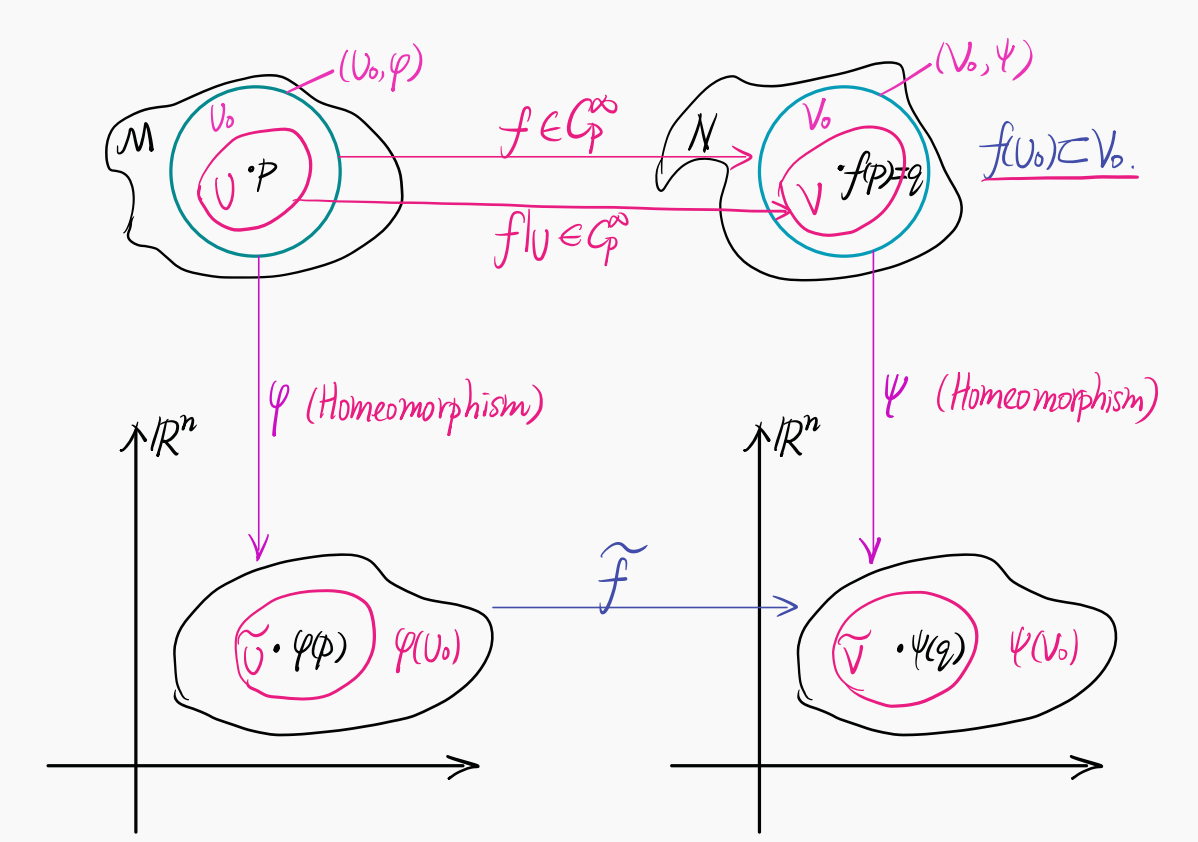
\includegraphics[width=0.6\textwidth]{figures/thm3.4.png}
            \end{center}
            \caption{图示}
            \label{fig:thm3.4proof}
        \end{small}
    \end{figure}
    
    故 $\tilde{f}=\psi\circ f\circ \varphi^{-1}$是光滑的. $\varphi(U_0)$与 $\psi(V_0)$均是 $\R^n$中的开集.在定理3.1中,令 $x_0=\varphi(p),f=\tilde{f}$,则若 $\det \left(\frac{\partial f^i}{\partial x^j}\right)\bigg|_{x_0}\neq 0$,则存在 $\varphi(p)$与$\psi(q)$在 $\varphi(U_0)$与 $\psi(V_0)$的邻域 $\widetilde{U}$与 $\widetilde{V}$,使得 $\tilde{f}|_{U_0}\colon \widetilde{U}\to\widetilde{V}$是可微同胚.
    令 $U=\varphi^{-1}(\widetilde{U}),V=\psi^{-1}(\widetilde{V})$,则 $U$与 $V$分别是$p$与 $q$在 $M$与 $N$中的邻域,且$f|_{U}=\psi^{-1}\circ \tilde{f}\circ \varphi\colon U\to V$是可微同胚.

    为何 $\tilde{f}$在 $\varphi(p)$的Jacobi行列式非零是显然的?
    由于
    \[
    \begin{aligned}
        & \left.\operatorname{det}\left(\frac{\partial f^i}{\partial x^j}\right)\right|_{x_0} \neq 0 . \Leftrightarrow f_*: T_{x_0} M\left(\simeq \mathbb{R}^n\right) \longrightarrow T_{f_{(x_0)}}\left(\mathbb{R}^n\right)\left(\simeq \mathbb{R}^n\right) \\
        & \left.\operatorname{det}\left(\frac{\partial \tilde{f}^i}{\partial x^j}\right)\right|_{\varphi(p)} \neq 0 \Leftarrow \tilde{f}_*: T_{\varphi(p)} M \left(\simeq \mathbb{R}^n\right) \longrightarrow T_{\tilde{f} \varphi(\rho)}\left(\mathbb{R}^n\right) (\simeq \mathbb{R}^n) 
        \end{aligned}\]
        故映射 $f$的 Jacobi矩阵 $\left(\frac{\partial f^i}{\partial x^j}\right)$恰是 $f_*$在自然基底下的矩阵.
\end{proof}
\subsection{小结}
\subsubsection*{余切空间}
\begin{itemize}
    \item 余切空间 $T^*_p =\F_p/\mathcal{H}_p=\{(\dd f)_p\}$,
    \item 自然基底 $\{(\dd u^i)_p,1\leqslant i\leqslant n\}$,
    \item 余切空间之间的光滑映射:
    \[F^*\colon T^*_q\to T^*_p\; \text{(设 $F\colon M\to N$是光滑映射且 $q=F(p)$.)}\]
    \begin{itemize}[label=\twicecircle]
        \item 作用方式 \quad $(\dd f)_p\mapsto \dd(f\circ F)$,
        \item 在两个自然基底下的矩阵表示: 
        
        设 $u^i$是 $p$附近的局部坐标表示, $v^\alpha$是 $q$附近的局部坐标表示,则映射 $F$在点$p$附近可用函数
        \begin{equation}
            \label{eq:valpha}
            v^\alpha=F^\alpha (u^1,\cdots,u^m),1\leqslant \alpha\leqslant n,
        \end{equation}
        表示.

        注解: \begin{eq*}
            v^\alpha &=(\psi(q))^\alpha=(\psi\circ F(p))^\alpha=(\psi\circ F\circ \varphi^{-1}(u^1,\cdots,u^m))^\alpha\\
            &\xlongequal[]{\text{令 $F^\alpha=\psi\circ F\circ \varphi^{-1}$}} F^\alpha (u^1,\cdots,u^m)
        \end{eq*}
        因此, $F^*$在自然基底 $\{\dd v^\alpha,1\leqslant\alpha\leqslant n\}$作用下结果为
        \begin{eq*}
                    F^* (\dd v^\alpha)=\dd (v^\alpha\circ F)=(\dd (F^\alpha(u^1,\cdots,u^m)))_p=\sum_{i=1}^{m}\left(\frac{\partial F^\alpha}{\partial u^i}\right)_p \cdot (\dd u^i).
        \end{eq*}
        从而 $F^* \{\dd v^\alpha\}=J\{\dd u^i\}$,其中 $J=\left(\frac{\partial F^\alpha}{\partial u^i}\right)_p$为 \eqref{eq:valpha}函数的Jacobi矩阵.
    \end{itemize}
    \item 余切向量的自然基底表示
    
    设 $\alpha=\dd f\in T_p^*$,则 $\alpha=\sum_{i=1}^{m}a_i \dd u^i, a_i=\frac{\partial f}{\partial u^i} \quad (\text{这里将复合映射仍记为$f$},  f=f\circ \varphi_U^{-1})$ (由定理 2.2)
    \item 坐标变换 (在不同坐标系$u^i$与$u^{*i}$下同一向量坐标变化)
    
    设另一局部坐标$u^{*i}$,则$\alpha$关于自然基底的表示式为$\alpha=\sum_{i=1}^{m}a_i^* \dd u^{*i}$,其中$a_i=\sum_{i=1}^{m}a_j^* \frac{\partial u^{*j}}{\partial u^i}$,且 $\frac{\partial u^{*j}}{\partial u^i}=\frac{\partial (\varphi_{U*}\circ \varphi_U^{-1})}{\partial u^i}$那么
    \begin{eq}
        \alpha &=(\dd u^1,\cdots,\dd u^m)\overrightarrow{\beta}, \overrightarrow{\beta}=(a_1,\cdots,a_m)^\prime \\ 
        &=(\dd u^{*1},\cdots,\dd u^{*m})\overrightarrow{\beta^*}, \overrightarrow{\beta}=(a_1^*,\cdots,a_m^*)^\prime
    \end{eq}
    又
    \begin{eq*}
        (\dd u^{*1},\cdots,\dd u^{*m})&=(\dd u^1,\cdots,\dd u^m)T\\
        &=(\dd u^1,\cdots,\dd u^m)(T\overrightarrow{\beta^*})
    \end{eq*}
即有$T\overrightarrow{\beta^*}=\overrightarrow{\beta}$.
由$T=\left(\frac{\partial u^{*j}}{\partial u^i}\right)\bigg|_{(ij)}$,故 $a_i=\sum_{i=1}^{m}a_j^* \cdot \left(\frac{\partial u^{*j}}{\partial u^i}\right)$.
\end{itemize}
\begin{remark}
    \begin{enumerate}[font=\upshape]
        \item $u^i (1\leqslant i\leqslant m)$称为点 $q\in U$ ($U$为$p$在$M$中的邻域)的局部坐标,即
        \begin{eq*}
            u^i=(\varphi_U(q))^i,\quad q\in U, 1\leqslant i\leqslant m
        \end{eq*}
        \item \Figure{width=.5\linewidth}{figures/11.png}{余切空间图示}{fig:cotangent space}
    \end{enumerate}
\end{remark}
\subsubsection*{切空间}
\begin{itemize}
    \item 切空间 $T_p=\{\langle [\gamma], (\dd f)_p\rangle, \gamma\in \Gamma_p\}$.
    \item 自然基底 $\{[\lambda_k],1\leqslant k\leqslant m\}=\left\{\left(\frac{\partial}{\partial u^k}\right)_p, 1\leqslant k\leqslant m\right\}$.
    \item 切空间之间的光滑映射 ($F^*$的共轭映射)(也称为相伴映射)
    \[F_*\colon T_p\to T_q,\]
    \begin{itemize}[label=\twicecircle]
        \item 作用方式: $\langle F_* X,\alpha\rangle=\langle X,F^* \alpha\rangle, X\in T_p,\alpha\in T_q^*$.
        \item 在两个自然基底下的矩阵表示
        
        切映射$F_*$在自然基底$\left\{\frac{\partial }{\partial u^i}\right\}$上的作用是
        \begin{eq}
            \langle F_*\left(\frac{\partial }{\partial u^i}\right),\dd v^\alpha\rangle &=\lan{\frac{\partial}{\partial u^i},F^*(\dd v^\alpha)}\\ 
            &=\sum_{i=1}^{m}\lan{\frac{\partial }{\partial u^i},\dd u^i}\cdot \left(\frac{\partial F^\alpha}{\partial u^i}\right)_p\\ 
            &=\lan{\sum_{i=1}^{m}\left(\frac{\partial F^\beta}{\partial u^i}\right)_p \frac{\partial }{\partial v^\beta},\dd v^\alpha}.
        \end{eq}
        即 $F_*\left(\frac{\partial }{\partial u^i}\right)=\sum_{\beta=1}^{m}\left(\frac{\partial F^\beta}{\partial u^i}\right)_p \frac{\partial }{\partial v^\beta}$.
    \end{itemize}
        \item 切向量的自然基底表示
        \[[\gamma]=X=\sum_{i=1}^{m}\xi^i \frac{\partial }{\partial u^i}, \xi^i=\frac{\dd (u^i\circ v)}{\dd t},\gamma\in \Gamma_p.\]
        \item 坐标变换
        
        设有另一局部坐标$u^{*i}$,则
        \begin{eq}
            X &=\left(\frac{\partial }{\partial u^1},\cdots,\frac{\partial }{\partial u^m}\right)\overrightarrow{\ell}, \overrightarrow{\ell}=\left(\xi^1,\cdots,\xi^m\right)^\prime\\ 
            &=\left(\frac{\partial }{\partial u^{*1}},\cdots,\frac{\partial }{\partial u^{*m}}\right)\overrightarrow{\ell^*}, \overrightarrow{\ell}=\left(\xi^{*1},\cdots,\xi^{*m}\right)^\prime
        \end{eq}
        由于 $\left(\frac{\partial }{\partial u^{*1}},\cdots,\frac{\partial }{\partial u^{*m}}\right)=\left(\frac{\partial }{\partial u^1},\cdots,\frac{\partial }{\partial u^m}\right)T$,故 $T\overrightarrow{\ell^*}=\overrightarrow{\ell}\implies \overrightarrow{\ell^*}=T^{-1}\overrightarrow{\ell}$,其中$T=\left(\frac{\partial u^{*j}}{\partial u^i}\right)_{(ij)}$,故 $\xi^{*j}=\sum_{i=1}^{m}\left(\frac{\partial u^{*j}}{\partial u^i}\right)\cdot \xi^i$,从而
        \[\sum_{j=1}^{m}\left(\partial \frac{u^{*i}}{\partial u^j}\cdot \xi^j\right)=\sum_{i=1}^{m}\left(\partial \frac{u^{*j}}{\partial u^i}\cdot \xi^i\right).\]
\end{itemize}
\begin{thm}
    设 $M$是 $m$维光滑流形, $N$是 $n$维光滑流形, $m<n$,设 $f\colon M\to N$是光滑映射. 若切映射$f_*$在点$p\in M$是非退化的(即$f_*$在点$p$是单一映射,此时$m\leqslant n$且$f_*$的Jacobi矩阵的秩为$m$,即$f_*$的Jacobi行列式非零),则存在点$p$的局部坐标系$(U;u^i)$及点$q=f(p)$的局部坐标系$(V;v^\alpha)$,使得$f(U)\subset V$,且$f|U$可用局部坐标表示为: $\forall x\in U$,有
    \begin{eq}
        \left\{\begin{array}{ll}
            v^i\circ f(x)=u^i (x), & 1\leqslant i\leqslant m,\\ 
            v^\gamma\circ f(x)=0, & m+1\leqslant \gamma\leqslant n.
        \end{array}\right.
    \end{eq}
\end{thm}
\begin{proof}
    设$f$
在点$p$的局部坐标系$(U;u^i)$与点$q$的局部坐标系$(V;v^\alpha)$下表示为
\[v^\alpha=f^\alpha(u^1,\cdots,u^m), 1\leqslant \alpha\leqslant n.\]
假定 $u^i (p)=0,v^\alpha (q)=0$. 因为$f_*$在点$p$是非退化的,则
\[\frac{\partial (f^1,\cdots,f^m)}{\partial (u^1,\cdots,u^m)}\bigg|_{n^i=0}\neq 0.\]
由于$f_*$在点$p\in M$是非退化的,则$f_*$的Jacobi行列式 $\det\left(\frac{\partial f^\alpha}{\partial u^i}\right)\bigg|_{p}\neq 0$.令上述行列式为$J_{m\times n}, 1\leqslant i\leqslant m,1\leqslant \alpha\leqslant n$,且 $m\leqslant n, \operatorname{rank}(J)=m$, 如下图所示
\begin{align}
    \left[
    \begin{tabular}{cccc|c}
        \multicolumn{4}{c}{}& \\
        \multicolumn{4}{c}{非奇异矩阵}&\\ 
        \multicolumn{4}{c}{$\frac{\partial (f^1,\cdots,f^m)}{\partial (u^1,\cdots,u^m)}$}&\\ 
        \multicolumn{4}{c}{}& \\
    \end{tabular}\right]
\end{align}
令$I_{n-m}=\left\{(\omega^{m+1},\cdots,\omega^{n})\mid |\omega^\gamma|<\delta,m+1\leqslant \gamma\leqslant n\right\} (\delta>0)$.
\begin{eq}
    f\colon U\to V & v^\alpha\colon f\to (f^1,\cdots,f^n)\\ 
    p\mapsto f(p)=q & q\mapsto (v^1,\cdots',v^n)
\end{eq}
将 $f(p)$用 $v^\alpha$作局部坐标表示为 
\[v^\alpha=(f(p))^\alpha=(f(u^1,\cdots,u^m))^\alpha=f^\alpha(u^1,\cdots,u^m),1\leqslant \alpha\leqslant n.\]
假定 $u^i (p)=0,v^\alpha (q)=0$, 因为由 $f$诱导的切映射 $f_*$ 是非退化的,即 $m\leqslant n$且$f_*$的Jacobi矩阵秩为$m$,即
\[
  \frac{\partial (f^1,\cdots,f^m)}{\partial (u^1,\cdots,u^m)}\neq 0,
\]
且
\begin{eq*}
    J_{m\times n}=\left(\frac{\partial f^\alpha}{\partial u^i}\right)_p=\frac{\partial (f^1,\cdots,f^m,f^{m+1},\cdots,f^n)}{\partial (u^1,\cdots,u^m)},1\leqslant i\leqslant m,1\leqslant \alpha\leqslant n.
\end{eq*}
\end{proof}
\begin{remark}
    扩充行空间为$n$维即引入$n-m$个维度将$(u^1,\cdots,u^m)$扩展为$(u^1,\cdots,u^m,\omega^{m+1},\cdots,\omega^n)$,并且满足
    定义光滑映射 $\widetilde{f}\colon U\times I_{n-m}\to V$,
    \begin{eq}
        \widetilde{f}^i (u^1,\cdots,u^m,\omega^{m+1},\cdots,\omega^n)&=f^i (u^1,\cdots,u^m) (\text{和原来的$f^i$相同}\quad 1\leqslant i\leqslant m),\\ 
        \widetilde{f}^i (u^1,\cdots,u^m,\omega^{m+1},\cdots,\omega^n)&=\omega^\gamma+f^\gamma(u^1,\cdots,u^m),m+1\leqslant \gamma\leqslant n.
    \end{eq} 
    则显然$\widetilde{f}$在$(u^i,\omega^\gamma)=(0,0)$的Jacobi行列式是非退化的,因为 
    \begin{eq*}
    J_{n\times n}^\prime =\left(\frac{\partial(\widetilde{f}^1,\cdots,\widetilde{f}^n)}{\partial(u^1,\cdots,u^m,u^{m+1},\cdots,u^n)}\right)\neq 0,\quad \ell=\left\{\begin{array}{ll}u,&1\leqslant i\leqslant m,\\ \omega,& m+1\leqslant\gamma\leqslant n.\end{array}\right.
    \end{eq*}
    \begin{align}
        |J^\prime|=\begin{vmatrix}
            \frac{\partial \widetilde{f}^1}{\partial u^1} & \cdots &\frac{\partial \widetilde{f}^m}{\partial u^1} & \frac{\partial \widetilde{f}^{m+1}}{\partial u^1} &\cdots & \frac{\partial \widetilde{f}^n}{\partial u^1}\\ 
            \vdots &&\vdots &\vdots &&\vdots\\
            \frac{\partial \widetilde{f}^1}{\partial u^m} & \cdots &\frac{\partial \widetilde{f}^m}{\partial u^m} & \frac{\partial \widetilde{f}^{m+1}}{\partial u^m}& \cdots & \frac{\partial \widetilde{f}^n}{\partial u^m}\\[10pt]
            \frac{\partial \widetilde{f}^1}{\partial u^{m+1}} & \cdots &\frac{\partial \widetilde{f}^m}{\partial u^{m+1}} & \frac{\partial \widetilde{f}^{m+1}}{\partial u^{m+1}} &\cdots & \frac{\partial \widetilde{f}^n}{\partial u^{m+1}}\\ 
            \vdots &&\vdots &\vdots &&\vdots\\
            \frac{\partial \widetilde{f}^1}{\partial u^n} & \cdots &\frac{\partial \widetilde{f}^m}{\partial u^n} & \frac{\partial \widetilde{f}^{m+1}}{\partial u^n}& \cdots & \frac{\partial \widetilde{f}^n}{\partial u^n}
        \end{vmatrix}=\begin{vmatrix}
            A_m & B_{m\times n-m}\\ 
            C_{n-m\times m} & D_{n-m}
        \end{vmatrix}\neq0
    \end{align}
\end{remark}
\clearpage

\section{形式与函数芽}
\subsection{微分形式}\index{微分形式}
\begin{figure}[htbp]
    \centering
    \begin{tikzpicture}[>=stealth,spy using overlays= {rectangle, magnification=5, connect spies}] %spy using outlines= {circle, magnification=6, connect spies} %圆形放大镜
        \draw[gray!30,very thin] (-5,-1) grid (5,9);
        \draw[->,thin] (-5,0) -- (5,0) node[right] {$x$};
        \draw[->,thin] (0,-1) -- (0,9) node[left] {$y$};
        \foreach \x in {-5,...,5}{
            \node[below,gray,font=\small] at (\x,-1) {$\x$};
        }
        \foreach \y in {-1,...,9}{
            \node[left,gray,font=\small] at (-5,\y) {$\y$};
        }
        \draw[thick,blue,domain=-5:2.2,smooth] plot (\x,{e^\x}) node[right] {$f(x)=e^x$};
        \draw[thick,black,domain=-2:5] plot (\x,{\x+1}) node[above] {$f(x)=x+1$};
        \coordinate (intersection) at (0,1);
        \node[red,left] at (intersection) {$(0,1)$};
        \node[black] at (1,e) {$(1,e)$};
        \draw[very thick,cyan,->] (2,-0.5) -- (0.1,0.95);
        \draw[shift={(0,-2)},thick,teal,domain=0:5] plot (\x,{\x+1}) node[above] {$f_1(x)=x-1$};
        \draw[rotate=30,shift={(0,-0.64)},magenta,domain=-0.95:6.4,thick] plot (\x,{\x+1}) node[above] {$g_1(x)$};
        \shade[ball color=gray] (intersection) circle [radius=2pt];%(2pt)也行
        \coordinate (spypoint) at (0,1);% The point to be magnified
        \coordinate (magnifyglass) at (-3,5);% The point where to see
        \spy [gray!50, size=2.5cm] on (spypoint) in node[fill=white] at (magnifyglass);
    \end{tikzpicture}
    \label{fig:微分形式解说}
    \caption{微分形式解说}
\end{figure}
在$(0,1)$附近,两函数靠得很近,而在$(0,1)$该点上,两函数的变化完全一样,或者说\textbf{二者在该点的局部具有相似性}!而在实数的整体上,$f$和$g$是完全不同的.但是
这里的函数$f$和$g$有着同样的微分形式,因为局部放大图中看到,它们在$(0,1)$的附近几乎无法区分.

形象地说,假如在$(0,1)$上放置一个人,不管他踩在哪一条曲线上,他都感觉是站在$45^\circ$的斜坡上.而如果向下平移函数$g$,如图中青色直线所示,依然不会改变$g$在点$(0,1)$的斜率,感觉一模一样,所以微分形式不变.
不过,如果我们旋转函数$g$的图像,如图中粉色直线所示,则在点$(0,1)$的坡度就变陡峭了,这时斜率发生了变化,我们放置在该点处的人可能就站不稳了,那么新函数$g_1(x)$在$(0,1)$点的微分形式发生了变化.其根本原因在于局部的导数值发生了变化.
至此,我们对微分形式有了一个大致的感觉: 与\textbf{导数}相关.接下来说明如何定义微分形式.
% \begin{center}
%     \begin{tikzcd}
%     \text{实数域上的一元光滑函数}\ar[->,>=stealth,d]\\
%     \text{一元光滑函数芽}\ar[->,>=stealth,d]\\
%     \text{一元函数的$1$--形式}
%     \end{tikzcd}
% \end{center}
现在只看微分形式中的$1$--形式,分三步理解.首先,光滑实值函数在任意一点处都有无穷阶连续导函数.在这里,我们只考虑定义域为全体实数的函数. 如一次函数,二次函数,指数函数等等,都是定义在
全体实数上的一元光滑函数.不过光滑函数依然是一个整体的概念.微分形式是局部的观点,因此我们要想办法看一点的附近.遵循着这种局部化的思想,就有了" 芽"
这一充满了局部风格的概念.

\textbf{芽的思想,本质上是根据函数在一点附近的局部表现,对这些函数进行分类,即所谓的等价关系}
\begin{definition}[][芽][def:芽]
    芽是定义在拓扑空间上函数集合的一种等价关系.
    定义在拓扑空间上的两个函数$f$和$g$,在点$x$处属于同一支芽,当且仅当存在一个开集$S$,使得$S$包含点$x$,且在$S$上$f$和$g$的函数值处处相等.
\end{definition}
这里的 拓扑空间可以选择实数集,开集就是开区间之并,而点$x$就是定义函数芽和微分形式的地方.

一些重要的概念 (游戏规则)

$\ll \gamma,[f]\gg =\frac{\dd (f\circ \gamma)}{\dd t}\Bigg|_{t=0},[f]\in \mathscr{F}_p,\gamma\in \Gamma_p,-\delta< t< \delta$;

$\mathscr{F}_p=C_p^\infty/\sim=\{[f]|f\in C_p^\infty\},[f]=\{g\in C_p^\infty|f\sim g\}$;

$\Gamma_p=\{\gamma |\gamma\text{是$M$上过点$p$的参数曲线}\}$,其中\textbf{参数曲线}是指从$\R$上一开区间$I=(a,b)$到流形$M$的光滑映射.

接下来,利用上述概念构造一个映射$\tau\colon \Gamma_p \times \mathscr{F}_p\to \R$,它将$(\gamma,[f])$映到一个实值$\ll \gamma,[f]\gg$,且$\tau$关于$[f]$是线性的.

定义$\mathscr{H}_p=\{[f]\in\mathscr{F}_p| \ll \gamma,[f]\gg=0,\forall \gamma\in \Gamma_p\}$,则$\mathscr{H}_p$是$\mathscr{F}_p$的线性子空间.

\begin{theorem}
设$[f]\in\mathscr{F}_p$,对于包含$p$的容许坐标卡$(U,\varphi_U)$,令
\begin{equation*}
F(x^1,\cdots,x^n)=f\circ\varphi_U^{-1}(x^1,\cdots,x^n),
\end{equation*}
则$[f]\in\mathscr{H}_p$当且仅当
\begin{equation*}
\frac{\partial F}{\partial x^i}\Bigg|_{\varphi_U(p)}=0,\quad 1\leqslant t\leqslant n.
\end{equation*}
\end{theorem}

\begin{remark}
理解本定理的关键是熟悉里面各个对象间的关系,下面借助交换图解释说明他们之间的关系.
\begin{center}
\begin{tikzcd}
    t\in I=(a,b)\subseteq \R \rar[mapsto,"\gamma"] & q\in U\;(p\in U)\drar[mapsto,blue,swap,"\varphi_V=f"]\rar[mapsto,"\varphi_U"] & \varphi_U (q)=(x^1(t),\cdots,x^n(t))\in \R^n \dar[mapsto,"F=f\circ \varphi_U^{-1}"]\\ 
    && [magenta] f(q)=\varphi_V(q)=(u^1,\cdots,u^n)\in \R^n
\end{tikzcd}
\end{center}
其中,在$p$点附近有包含$p$点的两个局部坐标卡,分别为$(U,\varphi_U)$和$(V,\varphi_V)$,其中令$f=\varphi_V$.
从而$\varphi_U(q)=\varphi_U\circ \gamma(t)$,特别地, $\varphi_U(p)=\varphi_U\circ \gamma(0)$.故$x^i (t)=\left(\varphi_U(q)\right)^i=\left(\varphi_U\circ \gamma(t)\right)^i,\; 1\leqslant t\leqslant n$.
\end{remark}

\begin{theorem}[][][thm:1.22]
设$f^1,\cdots,f^n\in C_p^\infty$,而$F(y^1,\cdots,y^n)$是在点$(f^1(p),\cdots,f^n(p))\in \R^n$的邻域内的光滑函数,则$f=F(f^1,\cdots,f^n)\in C_p^\infty$,并且
\begin{equation*}
(df)_p=\sum_{k=1}^{s}\left(\frac{\partial F}{\partial f^k}\right)_{f(p)}\cdot (df^k)_p.
\end{equation*}
\end{theorem}

\begin{remark}
同理,绘制定理对应的对象间关系图如下:
\begin{center}
    \begin{tikzcd}
    q\in U \;(p\in U) \rar[mapsto,"\varphi_U"]\drar[mapsto,swap,"\varphi_V"]& \varphi_U(q)=(x^1,\cdots,x^n)\in \R^n \rar[mapsto,"f^i"]\dar[mapsto,"F"]& x^i\in \R ,\; 1\leqslant i\leqslant n \\ 
    &\varphi_V(q)=(u^1,\cdots,u^n)\in \R^n &
    \end{tikzcd}
\end{center}
其中,$x^i=f^i\circ \varphi_U(q)=f^i (x^1,\cdots,x^n)=\sum_{k=1}^{n}f^i(x^k)=\delta_k^i x^k$,其中$\delta_k^i$为Kronecker记号.则
\begin{align*}
(df)_p=dF(f^1(p),\cdots,f^n (p))&=\Dif{F(f^1\circ \gamma(t),\cdots,f^n\circ\gamma(t))}{t}\Bigg|_{t=0}\\ 
&=\sum_{k=1}^{n}\frac{\partial F}{\partial \left(f^k\circ \gamma(t)\right)}\Bigg|_{t=0}\cdot \Dif{\left(f^k\circ\gamma(t)\right)}{t}\Bigg|_{t=0}\\ 
&=\sum_{k=1}^{n}\frac{\partial F}{\partial f^k}\Bigg|_{(f^1(p),\cdots,f^k(p))}\cdot \left(\dd f^k\right)_p.
\end{align*}
\end{remark}

\begin{example}
设$\dim M=n$,试证明$\dim T_p^*=n$.
\end{example}
具体证明分两部分,首先,先通过余切向量的局部坐标表示得出$T_p^*$中任一向量的一个线性组合(当然,此时还不能成为基),然后,证明这个组合里的向量线性无关即可.此处不详细写出证明,仅谈论如何理解该证明的思路.

\begin{fancybox}
\begin{center}
\begin{tikzcd}
    &q\in U \dlar[mapsto,swap,"\varphi_V=f"]\dar[mapsto,"\varphi_U"]\drar[mapsto,"u^i"]&\\ 
    \varphi_V(q)=(u^1,\cdots,u^n)& \lar[mapsto,"F=f\circ\varphi_U^{-1}"]\varphi_U(q)=(x^1,\cdots,x^n)\in \R^n \rar[mapsto,"x^i"]& x^i\in\R,\; 1\leqslant i\leqslant n
\end{tikzcd}
\end{center}
其中, $u^i=x^i\circ \varphi_U\in C_p^\infty,(\dd u^i)_p\in T_p^*$.根据定理~\ref{thm:1.22},令$f^i=u^i,1\leqslant i\leqslant n$,得$ f=F(u^1(q),\cdots,u^n(q))\in C_p^\infty$,且对于任一$T_P^*$中的余切向量$(\dd f)_p$有
\begin{align*}
(\dd f)_p=\sum_{i=1}^{n}\left(\frac{\partial F}{\partial u^i}\right)_{(u^1(p),\cdots,u^n(p))}\cdot (\dd u^i)_p.
\end{align*}
由上式可知,$\{(\dd u^i)_p,1\leqslant i\leqslant n\}$是$T_p^*$中任一向量的一个线性组合基底.
接下来,证明它就是$T_P^*$的一个基,只需证明它们线性无关即可.
按照证明线性无关的一般准则,设存在一组实数$\alpha_i,1\leqslant i\leqslant n$,使得
\begin{equation*}
\sum_{i=1}^{n}\alpha_i (\dd u^i)_p=0,.
\end{equation*}
而
\begin{align*}
(\dd u^i)_p=\Dif{u^i\circ \gamma(t)}{t}\Bigg|_{t=0}.
\end{align*}
从而$\ll\gamma,[u^i]\gg=0$,即$[u^i]\in\mathscr{H}_p$.由于$\tau$对于第二个变量是线性的,故而
\[\ll \gamma,\sum_{i=1}^{n}\alpha_i [u^i]\gg=\sum_{i=1}^{n}\alpha_i \Dif{u^i\circ\gamma(t)}{t}\Bigg|_{t=0}=0,\color{red}{\forall \gamma\in\Gamma_p}.\]

关键在于上面标注的红色部分,\textbf{$\gamma$是可以任意取定的},从而,\color{purple}{为了能将上式与$\alpha_i=0$联系起来,我们可以设法确定一个非常特殊的函数$\gamma$,使得上式中的系数部分$\Dif{u^i\circ\gamma(t)}{t}\Bigg|_{t=0}=\delta_{k}^i$即可,而这也就是基底向量的正交性.} 经过多次尝试,我们可以作函数$\gamma=\lambda_k\in \Gamma_p$,使得
\begin{equation*}
u^i\circ\lambda_k(t)=u^i(p)+\delta_k^i t
\end{equation*}
经过验证,上述函数符合要求.
\end{fancybox}
\begin{fancybox}
\textbf{\textcolor[rgb]{0.88,0.15,0.33}{看懂与撰写证明的方法技巧}}
\begin{description}
    \item[\textbf{Step I.}] \textbf{理清证明的全局思维脉络 (化整为零)}~
    结合大纲、思维导图、逻辑组织架构图、树状图等等思维组织形式来把握整理整个证明流程的思路历程及关键环节、步骤,以及疏通条件与结论之间起桥梁作用的各个中间站点,明确它们的职能与权重。
    \item[\textbf{Step II.}] \textbf{斟酌微观的技术细节 (微观操作)}~
    透过回顾知识点、联想概念以及理论关联性来琢磨各个职能各异、权重参差的中间站点之间的联络方式,从而将其中的技术难点和微观层面的技术细节一一抠弄出来解决。
\end{description}
\end{fancybox}

\begin{theorem}[][Stokes 定理][thm: Stokes theorem]
    设 $M$ 是定向带边界的$n$维光滑流形, $\omega$ 是紧致的$(n-1)$--形式, 则
    \[\int_M \dd \omega=\int_{\partial M} \omega.\]
    特别的, 如果 $\partial M=\emptyset$, 则 $\int_M\dd \omega=0$.
\end{theorem}
\begin{proof}
取 $M$ 的坐标图册 $\left\{U_i\right\}_{i \in I}$, 其中每个开集都同胚于 $n$ 维空间或者闭半空间. 取支于其上的单位分解, 即 $M$ 上一族非负 光滑函数 $\left\{\varphi_i\right\}_{i \in I}$, 满足 $\varphi_i$ 支集紧,包含于 $U_i, M$ 上每点都有邻域上面只有有限个 $\varphi_i$ 非零, 以及 $\sum_{i \in I} \varphi_i=1$. 令 $\omega_i=\varphi_i \omega$, 则 $\sum_{i \in I} \omega_i=\omega$. 又由于 $\omega$ 紧支, 只有有限个 $\omega_i$ 非零, 于是只需对每个 $\omega_i$ 证明定理. 这样便只需证 $M$ 是 $n$ 维空间和闭半空 间的情形. 以下分别证之.

1. $M=\mathbb{R}^n$. 

此时写出 $\omega=\sum_{i=1}^n f_i d x_1 \wedge \cdots \wedge \widehat{d x_i} \wedge \cdots \wedge d x_n$, 其中 $\widehat{\phantom{d}}$ 表示不出现. 只需对求和中每一项证明定理; 置换坐标可 设只有第一项, 即 $\omega=f d x_2 \wedge \cdots \wedge d x_n$. 此时 $d \omega=\frac{\partial f}{\partial x_1} d x_1 \wedge \cdots \wedge d x_n$. 由 \textbf{Fubini 定理 (与积分运算可交换次序) 和微积分基本定理},
\begin{align*}
\text { 左边 }& =\int_{\mathbb{R}^{n-1}}\left(\int_{\mathbb{R}} \frac{\partial f}{\partial x_1} d x_1\right) d x_2 \cdots d x_n=\left.\int_{\mathbb{R}^{n-1}} f\left(\cdot, x_2, \ldots, x_n\right)\right|_{-\infty} ^{+\infty} d x_2 \cdots d x_n\\
&=\int_{\mathbb{R}^{n-1}} 0 d x_2 \cdots d x_n=0=\text { 右边, }
\end{align*}
因为 $f$ 紧支.

2. $M=\left\{x \in \mathbb{R}^n \mid x_1 \leq 0\right\}$.  

此时仍写 $\omega=\sum_{i=1}^n f_i d x_1 \wedge \cdots \wedge \widehat{d x_i} \wedge \cdots \wedge d x_n$. 仍只需对求和中每一项证明定理. 后 $n-1$ 项 的计算和上一段一样是 0 . 对第一项, 由\textbf{Fubini 定理 (与积分运算可交换次序) 和微积分基本定理},
\begin{align*}
\text { 左边 }&=\int_{\mathbb{R}^{n-1}}\left(\int_{-\infty}^0 \frac{\partial f}{\partial x_1} d x_1\right) d x_2 \cdots d x_n=\left.\int_{\mathbb{R}^{n-1}} f\left(\cdot, x_2, \ldots, x_n\right)\right|_{-\infty} ^0 d x_2 \cdots d x_n\\
&=\int_{0 \times \mathbb{R}^{n-1}} f d x_2 \cdots d x_n=\text { 右边, }
\end{align*}
由于带边流形的定向约定.
\end{proof}

\begin{definition}[][自由对象]
    我们首先给出一个具体范畴(concrete category) $\mC$ ,$F$是其中的一个对象, $X$是一个非空集合并且给出一个映射$i\colon X\to F$.  我们称$F$在集合$X$上自由(free),如果对任何$\mC$中的对象$A$和映射$f\colon X\to A$ ,我们都可以找到一个唯一$\mC$的上的态射$g\colon F\to A$使得 $gi=f$. 如下图所述:
    \begin{tikzcd}
        X\subset \mC \arrow[d,"i",swap]\arrow[r,"f"] & A\subset \mC \\ 
        F \arrow[ru,"g",swap] & 
    \end{tikzcd}
\end{definition}















\partabstract{《微分流形与李群基础》根据F. w., 瓦内尔所著Foundations of Diffrentiable Manifoldsand Lie Groups(Springer出版社1983年版)一书译出. 《微分流形与李群基础》特色鲜明、选材精练、论述精辟, 全书共分6章, 其核心材料主要包含在第1, 2, 4章中, 包括微分流形、微分形式、流形上的积分以及de Rham上同调等, 第3章则比较系统地论述了Lie群论的基本内容, 第5章论述de Rham定理并为此发展了公理化层上同调论, 第6章论述Hodge定理并以Fourier级数为基本工具给出了椭圆算子局部理论的完整论述, 这在一般参考书中是不容易找到的. }
\part{微分几何学}
\chapter{微分流形与李群基础}
\section{微分流形期末考试内容}
\subsection{证明题}
\begin{exam}
    证明 $n$ 维球面 $S^n=\{(x_1,\cdots,x_{n+1})\in\mathbb{R}^{n+1}\mid \sum_{i=1}^{n+1}x^2_i=1\}$ 是 $n$维 $C^\infty$ 微分流形.
\end{exam}
\begin{proof}
    取 $S^n$ 的拓扑为 $\R^{n+1}$ 子空间的拓扑, 则 $S^n$ 是Hausdorff空间.令
    \begin{equation}
        \begin{aligned}
            U^+_i &=\{(x_1,\cdots,x_{n+1})\in S^n\mid x_i>0\};\\
            U^-_i &=\{(x_1,\cdots,x_{n+1})\in S^n\mid x_i<0\}.\\
            \varphi_i^+ &\colon U_i^+ \to \R^n ,(x_1,\cdots,x_{n+1}) \to (x_1,\cdots,\hat{x_i},\cdots,x_{n+1});\\
            \varphi_i^- &\colon U_i^- \to \R^n ,(x_1,\cdots,x_{n+1}) \to (x_1,\cdots,\hat{x_i},\cdots,x_{n+1});
        \end{aligned}
    \end{equation}
    其中 $i=1,2,\cdots,n+1$,则 $\varphi_i^+$ 与 $\varphi_i^-$ 都是可逆映射,有
    \begin{equation*}
        \begin{aligned}
            (\varphi_i^+)^{-1} &\colon \varphi (U_i^+) \to U_i^+ , (x_1,\cdots,x_n) \mapsto (x_1,\cdots,x_{i-1},\sqrt{1-\sum_{j=1}^{n}x_j^2},x_i,\cdots,x_n);\\ 
            (\varphi_i^-)^{-1} &\colon \varphi (U_i^-) \to U_i^- , (x_1,\cdots,x_n) \mapsto (x_1,\cdots,x_{i-1},-\sqrt{1-\sum_{j=1}^{n}x_j^2},x_i,\cdots,x_n);
        \end{aligned}
    \end{equation*}
    考虑映射
    \begin{eq*}
        \varphi_2^{-1} (\varphi_1^+)^{-1}\colon \varphi_1^+ (U_1^+ \bigcap U_2^-)\to \varphi_2^{-1} (U_1^+\bigcap U_2^{-}) \\ 
        (x_1,\cdots,x_n)\mapsto \left(\sqrt{1-\sum_{j=1}^n x_j^2 },x_2,\cdots,x_n\right),
    \end{eq*}
    可知 $\varphi_2^{-1} (\varphi_1^+)^{-1}$ 是 $C^\infty$映射,因此坐标卡 $(U_1^+,\varphi_1^+)$ 和 $(U_2^-,\varphi_2^-)$ 是 $C^\infty$ 相容的. 同理可得坐标图册 $\left\{(U_i^{\pm},\varphi_i^{\pm})\mid i=1,2,\cdots,n+1\right\}$ 是 $C^\infty$相容坐标图册.因此唯一确定了 $S^n$ 上的 $C^\infty$ 微分结构, 故 $S^n$ 是 $n$ 维光滑流形.
\end{proof}

\begin{prop}
    $S^n$ 是 $n$ 维 $C^\omega$ 流形.
\end{prop}

\begin{proof}
    设 $p\in S^n\subset \R^{n+1}$,他的直角坐标系为 $(x^1,\cdots,x^{n+1})$, 如果将 $\R^n=\{(x^1,\cdots,x^n,0)\mid x^i\in\R,0\leqslant i\leqslant n\}\subset \R^{n+1}$与 $\R^n=\{(x^1,\cdots,x^n)\mid x^i\in\R,0\leqslant i\leqslant n\}\subset \R^{n+1}$ 视作相同的,则从图中容易算出:
    \begin{eq*}
        \varphi_1\colon U_1\to\R^n ,& (u^1,\cdots,u^n)=\varphi_1 (x^1,\cdots,x^{n+1})=\left(\frac{x^1}{1+x^{n+1}},\cdots,\frac{x^n}{1+x^{n+1}}\right);\\ 
        (x^1,\cdots,x^{n+1}) &= \varphi_1^{-1} (u^1,\cdots,u^n)=\left(\frac{2u^1}{1+\sum\limits_{i=1}^{n}(u^i)^2},\cdots,\frac{2u^n}{1+\sum\limits_{i=1}^{n}(u^i)^2},\frac{1-\sum\limits_{i=1}^{n}(u^i)^2}{1+\sum\limits_{i=1}^{n}(u^i)^2}\right)\\
        \varphi_2\colon U_2\to\R^n ,& (\overline{u}^1,\cdots,\overline{u}^n)=\varphi_2 (x^1,\cdots,x^{n+1})=\left(\frac{x^1}{1-x^{n+1}},\cdots,\frac{x^n}{1-x^{n+1}}\right);\\ 
        (x^1,\cdots,x^{n+1}) &= \varphi_2^{-1} (\overline{u}^1,\cdots,\overline{u}^n)=\left(\frac{2\overline{u}^1}{1+\sum\limits_{i=1}^{n}(\overline{u}^i)^2},\cdots,\frac{2\overline{u}^n}{1+\sum\limits_{i=1}^{n}(\overline{u}^i)^2},\frac{\sum\limits_{i=1}^{n}(\overline{u}^i)^2-1}{1+\sum\limits_{i=1}^{n}(\overline{u}^i)^2}\right)\\
    \end{eq*}
    且
    \begin{eq*}
        (\overline{u}^1,\cdots,\overline{u}^n)&=\left(\frac{u^1}{\sum\limits_{i=1}^n (u^i)^2},\cdots,\frac{u^n}{\sum\limits_{i=1}^n (u^i)^2}\right),\\ 
        (u^1,\cdots,\overline{u}^n)&=\left(\frac{\overline{u}^1}{\sum\limits_{i=1}^n (\overline{u}^i)^2},\cdots,\frac{\overline{u}^n}{\sum\limits_{i=1}^n (\overline{u}^i)^2}\right).
    \end{eq*}
    于是,  $\mathscr{D}_1^\prime=\{(U_1,\varphi_1),(U_2,\varphi_2)\}$满足定义1中的条件 (1): $S^n=U_1\bigcup U_2$
和条件 $\mathscr{D}_1^\prime$ 中元素是 $C^\omega$相容的 ($\{u^i\}$和 $\{\overline{u}^i\}$ 彼此可表示为实有理函数,由于实变量的有理函数可以自然延拓为复变量的有理函数,再由求导的加减乘除法则可知后者关于复变量是可导的,所以也是解析的. 于是它在每一点的一个开领域内可展开为收敛的幂级数.如果再限制在实变量,那么它在每一点的一个实的开领域上也可以展开为收敛的幂级数. 因此实有理数是实解析的.根据微分构造的定理, $\mathscr{D}_1^\prime$ 确定了 $S^n$上的一个 $C^\omega$ 微分构造 $\mathscr{D}_1=\{(U,\varphi)\mid (U,\varphi)\text{与} \mathscr{D}_1^\prime \text{是 $C^\omega$相容的}\}$ . 而 $\mathscr{D}_1^\prime$ 是 $C^\omega$微分构造 $\mathscr{D}_1$的一个基,通过计算可得Jacobi行列式为
\begin{eq*}
    J_{\varphi_2\circ \varphi_1^{-1}}=-\frac{1}{\left(\sum\limits_{i=1}^n (u^i)^2\right)^n},
\end{eq*}
如果将局部坐标 $\{\overline{u}^1,\overline{u}^2,\cdots,\overline{u}^n\}$ 换成 $\{\overline{u}^2,\overline{u}^1,\overline{u}^3,\cdots,\overline{u}^n\}$,则相应的Jacobi行列式大于零.
\clearpage
下面换一种方式来给出 $S^n$ 的 $C^\omega$微分构造的另一个基. 为此, 对任意 $i=1,2,\cdots,n+1$,令
\begin{eq*}
     U^+_i &=\{(x_1,\cdots,x_{n+1})\in S^n\mid x_i>0\};\\
            U^-_i &=\{(x_1,\cdots,x_{n+1})\in S^n\mid x_i<0\}.\\
            \varphi_i^+ &\colon U_i^+ \to \varphi_i^+ (U_i^+)=\left\{(x^1,\cdots,\hat{x^i},\cdots,x^{n+1})\mid \sum_{j\neq i} (x^j)^2<1\right\},\\
            \varphi_i^+ & (x^1,\cdots,x^{n+1})=(x^1,\cdots,\hat{x^i},\cdots,x^{n+1})
\end{eq*}
称 $(x^1,\cdots,\hat{x^i},\cdots,x^{n+1})$ 为 $U_i^+$中的局部坐标,其中 $\hat{x^i}$ 表示删去第 $i$项 $x^i$.

由此可以知道, $\mathscr{D}_1^\prime=\{(U_i^{\pm},\varphi_i^{\pm})\mid i=1,\cdots,n+1\}$满足微分构造的定义中的条件 (1): $S^n=\bigcup_{i=1}^{n=1} (U_i^+\bigcup U_i^-)$ 和条件 (2): $\mathscr{D}_2^\prime$中的元素是 $C^\omega$相容的.

例如, \begin{eq*}
\varphi_2^+\circ(\varphi_1^{-1})^{-1}(x^2,\cdots,x^{n+1}) &=\varphi_2^+ (x^1,\cdots,x^{n+1})=(x^1,\cdots,x^{n=1})\\ 
&=\left(-\sqrt{1-\sum_{i=1}^{n+1}(x^i)^2},x^3,\cdots,x^{n+1}\right)
\end{eq*}
是 $C^\omega$类的 (利用 $\sqrt{1-u}$在 $0$的开邻域 $(-1,1)$中可展开为收敛幂级数和. 由微分构造的定理可知, $\mathscr{D}_2^\prime$确定了 $S^n$上的一个 $C^\omega$微分构造 $\mathscr{D}=\{(U,\varphi)\mid (U,\varphi)\text{与 $\mathscr{D}_2^\prime$是 $C^\omega$相容的}\}$,而 $\mathscr{D}_2^\prime$是微分构造 $\mathscr{D}_2$的一个基.

通过计算得到Jacobi行列式为
\[    J_{\varphi_2\circ \varphi_1^{-1}}=-(-1)^{i+j}\frac{x^j}{x^i},\])
如果取 $(-1)^{i+1}\{x^1,\cdots,\hat{x^i},\cdots,x^{n+1}\}$为 $U_i^+$的局部坐标 ($(-1)^{i+1}\{x^1,\cdots,\hat{x^i},\cdots,x^{n+1}\}$表示将坐标 $\{x^1,\cdots,\hat{x^i},\cdots,x^{n+1}\}$做 $i+1$次对换 ),取 $(-1)^i\{x^1,\cdots,\hat{x^i},\cdots,x^{n+1}\}$为 $U_i^-$的局部坐标,则相应的Jacobi行列式大于零.

因为 $\{x^1,\cdots,x^{n+1}\}$ 与 $\{u^1,\cdots,u^n\}$ (或 $\{\overline{u}^1,\cdots,\overline{u}^n\}$)彼此可以表示出来,且 $\mathscr{D}_1^\prime$ 与 $\mathscr{D}_2^\prime$中的元素是 $C^\omega$相容的,由微分构造定理知 $\mathscr{D}_1=\mathscr{D}_2$.

因为紧致集 $S^n$不能与 $\R^n$中的开集同胚,所以 $S^n$不是局部坐标邻域.

此外,对于 $S^2$,球面坐标系 $(U,\varphi)\in \mathscr{D}_1=\mathscr{D}_2$,它是局部坐标系而不是整体坐标系,其中
\begin{eq*}
    \varphi^{-1}\colon (0,\pi)\times (0,2\pi) \to U=\varphi^{-1} ((0,\pi)\times (0,2\pi))\subset S^n,\\ 
    \varphi^{-1} (\theta,\varphi)=(\sin \theta\cdot \cos \varphi,\sin\theta\cdot \sin \varphi,\cos \theta).
\end{eq*}
对于 $S^1$,令
\begin{eq*}
    \psi_1\colon & S^1\to \{e^{i\theta}\}\to (0,2\pi)\subset \R^1 \\ 
    &\psi_1 (e^{i\theta})=\theta,\theta\in (0,2\pi),\\ 
    \psi_2\colon & S^1\to \{e^{i\eta}\}\to (\pi,3\pi)\subset \R^1 \\ 
    &\psi_2 (e^{i\eta})=\eta,\eta\in (\pi,3\pi).
\end{eq*}
显然,在 $S^1-\{e^{i\theta},e^{i\eta}\}$中, $e^{i\theta}=e^{i\eta}\iff \eta=\theta+2k\pi=\begin{cases}
    \theta+2\pi, &\theta\in (0,2\pi)\\ 
    \theta, & \theta\in (\pi,2\pi)
\end{cases}$,于是 $\eta$ 是 $\theta$的 $C^\omega$函数, $\theta$ 也是 $\eta$的 $C^\omega$函数. 由w由微分构造定理知, $\mathscr{D}_3^\prime=\{(S^1-\{e^{i\theta}\},\psi_1),(S^1-\{e^{i\eta}\},\psi_2)\}$确定了一个 $1$维 $C^\omega$微分构造 $\mathscr{D}_3\colon \mathscr{D}_1=\mathscr{D}_2=\mathscr{D}_3$.(注: $\theta$是局部坐标系而非整体坐标系)
)
\end{proof}
\begin{exam}
    证明实射影空间是微分流形.
\end{exam}
\begin{proof}
    $n$维实射影空间 (定义): 设 $x=(x^1,\cdots,x^{n+1},y=(y^1,\cdots,y^{n+1})\in \R^{n+1}-\{0\},x\sim y \iff x=\lambda y,0\neq\lambda\in \R$. $x\in\R^{n+1}-\{0\}$的等价类 $[x]=\{y\in\R^{n+1}-\{0\}\mid y\sim x\}$.等价类的全体构成
    \begin{eq*}
        \R P^n=(\R^{n+1}-\{0\})\backslash \sim=\left\{[x]\mid x\in\R^{n+1}-\{0\}\right\}
    \end{eq*}
    投影 $\pi\colon \R^{n+1}-\{0\}\to\R P^n, \pi (x)=[x]$.设 $\R^{n+1}-\{0\}$的拓扑为 $\tau$,可得 $\tau^\prime=\{U\mid \pi^{-1}(U)\in\tau\}$为 $\R P^n$上的一个拓扑,于是 $(\R P^n,\tau^\prime)$为 $(\R^{n+1}-\{0\},\tau)$的上空间,称为 $n$ 维实射影空间.

    下面证明 $\R P^n$ 为 $n$ 维 $C^\omega$流形.
% \footimage{liuhui.jpg}
% \foottext{Mathematics is a variety of proof techniques.}
    对任意的 $[x],[y]\in\R P^n$, 且 $[x]\neq [y]$,则存在含 $\pi^{-1} ([x])$的\textbf{以原点为心的去心开锥体 $V_y$},使得 $V_x\bigcap V_y=\emptyset$,因而 $\pi (V_x)$和 $\pi(V_y)$分别是含 $[x]$和 $[y]$的不相交开集,所以 $(\R P^n,\tau^\prime)$是 $T^2$空间.令
    \begin{eq*}
        U_k &=\{[x]\in\R P^n\mid x=(x^1,\cdots,x^{n+1}),x^k\neq 0\}, \\ 
        \varphi_k &\colon U_k\to \R^n,\\ 
        \varphi_k ([x])&=\left(\frac{x^1}{x^k},\cdots,\frac{x^{k-1}}{x^k},\frac{x^{k+1}}{x^k},\cdots,\frac{x^{n+1}}{x^k},\right)\\ 
        &=\left({}_k \xi^1,\cdots,{}_k \xi^{k-1},{}_k \xi^{k+1},\cdots,{}_k \xi^{n+1}\right).
    \end{eq*}
    我们称 $(x^1,\cdots,x^{n+1})$为 $[x]$的齐次坐标, $\left({}_k \xi^1,\cdots,{}_k \xi^{k-1},{}_k \xi^{k+1},\cdots,{}_k \xi^{n+1}\right)$为 $[x]$ 关于 $U_k$的非齐次坐标.

    显然, $\bigcup_{k=1}^n U_k=\R P^n$,当 $U_k \bigcap U_l\neq \emptyset,k\neq l$时,
    \begin{eq*}
        \varphi_l\circ \varphi_k^{-1}&\colon \varphi_k (U_k\bigcap U_l)\to \varphi_l (U_k\bigcap U_l) \\ 
        \varphi_l\circ \varphi_k^{-1} &\left({}_k \xi^1,\cdots,{}_k \xi^{k-1},{}_k \xi^{k+1},\cdots,{}_k \xi^{n+1}\right)=\varphi_l([x])=\left({}_l \xi^1,\cdots,{}_l \xi^{l-1},{}_l \xi^{l+1},\cdots,{}_l \xi^{n+1}\right).
    \end{eq*}
    其中
    \begin{eq*}
        \begin{cases}
            {}_l\xi^h =\frac{x^h}{x^l}=\frac{x^h}{x^k}/\frac{x^l}{x^k}=\frac{{}_k\xi^h}{{}_k\xi^l},h\neq l,k,\\ 
            {}_l\xi^k=\frac{x^k}{x^l}=1/\frac{x^l}{x^k}=1/{}_k\xi^l.
        \end{cases}
    \end{eq*}
    为有理数,因而它是 $C^\omega$函数. 由微分构造的定理知
    $\mathscr{D}^\prime=\{(U_k,\varphi_k)\mid k=1,\cdots,n+1\}$确定了 $\R P^n$上的一个 $C^\omega$微分结构 $\mathscr{D}$,使得 $(\R P^n,\mathscr{D})$成为 $C^\omega$流形.

    通过计算得Jacobi行列式为
    \begin{eq*}
        J_{\varphi_l\circ \varphi_k^{-1}}&=\frac{\partial \left({}_l \xi^1,\cdots,{}_l \xi^{l-1},{}_l \xi^{l+1},\cdots,{}_l \xi^{n+1}\right)}{\partial \left({}_k \xi^1,\cdots,{}_k \xi^{k-1},{}_k \xi^{k+1},\cdots,{}_k \xi^{n+1}\right)}\\ 
        &=(-1)^{l+k}\frac{1}{({}_k\xi^l)^{n+1}}.
    \end{eq*}
    当 $n$ 为奇数时, $({}_k\xi^l)^{n+1}>0$,如果 $k$为奇数, 相应的局部坐标不变;如果 $k$为偶数,相应的局部坐标只改变其中一个,即 ${}_k\xi^s$变为 $-{}_k \xi^s$,其余不变,且局部坐标改变后的Jacobi行列式大于零. 当 $n$为偶数时,由于 ${}_k\xi^l$有正有负,所以 $J_{\varphi_l\circ \varphi_k^{-1}}$也有正有负.
\end{proof}
\begin{defi}[子流形]
\begin{enumerate}[label=(\Roman*)]
    \item 如果 $d\psi_m$ 对于每一个 $m\in M$ 都是非奇异的, 那么 $\psi$ 是一个浸入(Immersion)或嵌入(Imbedding).
    \item 如果 $\psi$ 是一一浸入, 那么偶 $(M,\psi)$ 是 $N$ 的一个子流形.
\end{enumerate}
\end{defi}
\subsection{第11题两小问}
\begin{defi}
    令 $\varphi\colon M\to N$ 是 $C^\infty$ 的, 对于 $M$ 上的光滑向量场 $X$ 和 $N$ 上的光滑向量场 $Y$, 如果 $\dd \varphi\circ X=Y\circ \varphi$,则称它们是 $\varphi$ 相关的.
\end{defi}
\begin{prop}\label{prop:relevant}
    令 $\varphi\colon M\to N$ 是 $C^\infty$ 的,且设 $X$ 和 $X_1$ 是 $M$ 上的光滑向量场;$Y$ 和 $Y_1$ 是 $N$ 上的光滑向量场. 如果 $X$ 和 $Y$ 是 $\varphi$相关的, $X_1$ 和 $Y_1$ 是 $\varphi$相关的,那么 $[X,X_1]$ 和 $[Y,Y_1]$ 也是 $\varphi$相关的.
\end{prop}
\begin{proof}
    必须证明 $\dd \varphi\circ [X,X_1]=[Y,Y_1]\circ \varphi$.为此令 $m\in M$且 $f\in C^\infty (N)$,那么必须证明
    \[\dd \varphi([X,X_1]_m)(f)=[Y,Y_1]_{\varphi(m)}(f).\]
    直接展开定义式即得
    \begin{eq}
        \dd\varphi([X,X_1])_{m}(f)&=[X,X_1]_m (f\circ \varphi)\\ 
        &=X_m (X_1(f\circ\varphi))-X_1|_m (X(f\circ \varphi))\\ 
        &=X_m ((\dd\varphi\circ X_1)(f))-X_1|_m ((\dd\varphi\circ X)(f))\\
        &=X_m(Y_1(f)\circ \varphi)-X_1|_m (Y(f)\circ \varphi)\\
        &=\dd\varphi(X_m)(Y_1(f))-\dd\varphi(X_1|_m)(Y(f))\\
        &=Y_{\varphi(m)}(Y_1(f))-Y_1|_{\varphi(m)}(Y_1(f))\\
        &=[Y,Y_1]_{\varphi(m)}(f).
    \end{eq}
\end{proof}
\begin{prop}
    两个左不变向量场的Lie括号自身也是一个左不变向量场.
\end{prop}
\begin{proof}
    在开始证明之前,我们先证明一个引理:
    \begin{lem}
        左不变向量场都是光滑的.
    \end{lem}
    \begin{proof}
        令 $X\in \mathfrak{G}$,令 $f\in C^\infty$.只需证明 $Xf\in C^\infty(G)$.由于
        \begin{eq}
            Xf(\sigma)=X_\sigma f=\dd l_\sigma (X_e)f=X_e (f\circ l_\sigma).
        \end{eq}
        因而需要证明 $\sigma\mapsto X_e (f\circ l_\sigma)$是 $G$ 上的 $C^\infty$函数.通过把这个函数表示成 $C^\infty$映射的适当复合来做到这一点.令 $G\times G\to G$表示群的乘法, $\varphi(\sigma,\tau)=\sigma\tau$.而且令 $i_e^1$和 $i_\sigma^2$是由
        \begin{eq}
            \begin{cases}
                i_e^1 (\tau)=(\tau,e),\\ 
                i_\sigma^2(\tau)=(\sigma,\tau).
            \end{cases}
        \end{eq}
        定义的 $G\to G\times G$的映射.令 $Y$ 是 $G$上使得 $Y(e)=X(e)$的任何 $C^\infty$向量场,那么 $(0,Y)$是 $G\times G$上的光滑向量场,而且 $[(0,Y)(f\circ \varphi)]\circ i_e^1$是 $G$上的 $C^\infty$函数.利用习题
        \begin{exam}
            考虑带有标准射影 $\pi_1\colon M\times N\to M$和 $\pi_2\colon M\times N\to N$的积流形 $M\times N$.\
            \begin{enumerate}[label=(\alph*),font=\upshape]
                \item 证明 $\alpha\colon \hat{M}\to M\times N$是 $C^\infty$的当且仅当 $\pi\circ \alpha$和 $\pi_2\circ \alpha$是 $C^\infty$的.
                \item 证明映射 $\nu \mapsto (\dd \pi_1 (\nu),\dd\pi_2(\nu))$是 $(M\times N)_{(m,m)}$与 $M_m\oplus N_n$的一个同构.
                \item 令 $X$和 $Y$分别是 $M$和 $N$上的 $C^\infty$向量场,那么由 $(b),X$和 $Y$规范地决定 $M\times N$上的向量场 $\hat{X}=(X,0)$和 $\hat{Y}=(0,Y)$. 证明 $[\hat{X},\hat{Y}]=0$.
                \item 令 $(m_0,n_0)\in M\times N$,并且
                \begin{eq}
                    i_{n_0}(m)&=(m,n_0),\\
                    i_{m_0}(n)&=(m_0,n).
                \end{eq}
                定义内射 $i_{n_0}\colon M\to M\times N$和 $i_{m_0}\colon N\to M\times N$.令 $\nu\in (M\times N)_{(m_0,n_0)}$,令 $\nu_1=\dd \pi_1 (\nu)\in M_{m_0},\nu_2=\dd \pi_2 (\nu)\in N_{n_0}$.令 $f\in C^\infty (M\times N)$.证明
                \[\nu (f)=\nu_1 (f\circ i_{n_0})+\nu_2 (f\circ i_{m_0})\]
            \end{enumerate}
        \end{exam}
        中的 $(d)$项,得出
        \begin{align*}
            [(0,Y)(f\circ \varphi)]\circ i_e^1(\sigma) &=(0,Y)_{(\sigma,e)}(f\circ \varphi)\\ 
            &=0_\sigma (f\circ \varphi\circ i_e^1)+Y_e(f\circ \varphi\circ i_\sigma^2)\\ 
            &=X_e(f\circ\varphi\circ i_\sigma^2)=X_e(f\circ l_\sigma).
        \end{align*}
        因而 $\sigma\to X_e (f\circ l_\sigma)$是 $G$上的光滑函数.这就证明了 $(b)$成立.
    \end{proof}
    % \footimage{R-C.jpg}
    % \foottext{Mathematics has abused me thousands of times, and I have never seen it before.}
    由引理可知, 左不变向量场都是光滑的,所以它们的Lie括号有定义.如果 $X$是与其自身 $l_\sigma$相关的,并且 $Y$也是与其自身 $l_\sigma$相关的,那么根据命题\ref{prop:relevant}
    $[X,Y]$就 $l_\sigma$相关于 $[X,Y]$.因而两个左不变向量场的Lie括号还是一个左不变向量场.
\end{proof}

\begin{prop}
    For any smooth $n$--manifold $M$, the tangent bundle $TM$ has a natural topology and smooth structure taht make it into a $2n$--dimensional smooth manifold. With respect to this structure , the projection $\pi\colon TM\to M$ is smooth.
\end{prop}
\begin{proof}
    We begin by defining the maps that will become our smooth charts. Given any smooth chart $(U,\varphi)$ for $M$, note that $\pi^{-1}(U)\subseteq TM$ is the set of all tangent vectors to $M$ at all points of $U$. Let $(x^1,\cdots,x^n)$ denote the coordinate fuctions of $\varphi$, and define a map $\widetilde{\varphi}\colon \pi^{-1}(U)\to \R^{2n}$ by
    \begin{equation}
    \label{eq:natural coordinates on TM}\widetilde{\varphi}\left(v^i\frac{\partial}{\partial x^i}\bigg|_p\right)=(x^1,\cdots,x^n(p),v^1,\cdots,v^n).
    \end{equation}
    see \textbf{Figure~\ref{fig:coordinate for tangent bundle}}
    \begin{figure}[ht]
        \centering
        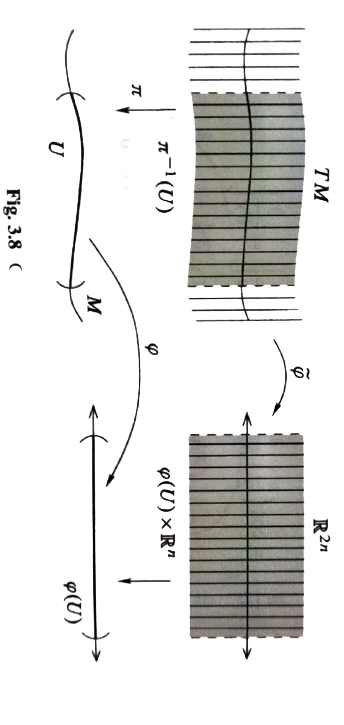
\includegraphics[angle=90,width=.7\linewidth]{figures/fog3.8.png}
        \caption{\textbf{Coordinate For the tangent bundle}}
        \label{fig:coordinate for tangent bundle}
    \end{figure}
    Its image set is $\varphi(U)\times\R^n$, which is an open subset of $\R^{2n}$. It is a bijection onto its image, because its inverse can be written explicitly as 
    \[\widetilde{\varphi}^{-1}(x^1,\cdots,x^n,v^1,\cdots,v^n)=v^i\frac{\partial}{\partial x^i}\bigg|_{\varphi^{-1}(x)}.\]
    Now suppose we are given two smooth charts $(U,\varphi)$ and $(V,\psi)$ for $M$, and let $(\pi^{-1}(U),\widetilde{\varphi}),(\pi^{-1}(V),\widetilde{\psi})$ be the corresponding charts on $TM$. The sets
    \begin{eq*}
        \widetilde{\varphi}\left(\pi^{-1}(U)\bigcap \pi^{-1}(V)\right)&=\varphi(U\bigcap V)\times \R^n \quad \textrm{and} \\ 
        \widetilde{\psi}\left(\pi^{-1}(U)\bigcap \pi^{-1}(V)\right)&=\psi(U\bigcap V)\times \R^n
    \end{eq*}
    are open in $\R^{2n}$, and the transition map $\widetilde{\psi}\circ \widetilde{\varphi}^{-1}\colon \varphi(U\bigcap V)\times \R^n\to \psi (U\bigcap V)\times \R^n$ can be written explicitly using 
    \begin{eq}
    \widetilde{v}^j=\frac{\partial \widetilde{x}^j}{\partial \widetilde{x}^i}(\hat{p})v^i
    \end{eq}
    as 
    \begin{eq*}
        \widetilde{\psi}&\circ \widetilde{\varphi}^{-1}(x^1,\cdots,x^n,v^1,\cdots,v^n) 
        =\left(\widetilde{x}^1 (x),\cdots,\widetilde{x}^n (x),\frac{\partial \widetilde{x}^1}{\partial \widetilde{x}^j}(x)v^j,\cdots,\frac{\partial \widetilde{x}^n}{\partial \widetilde{x}^j}(x)v^j\right)
    \end{eq*}
    This is clearly smooth.

    Choosing a countable cover $\{U_i\}$ of $M$ by smooth coordinate domains, we obtain a countable cover of $TM$ by coordinate domains $\{\pi^{-1}(U_i)\}$ satisfying conditions (i)-- (iv) of the smooth manifold chart lemma (Lemma 1.35). To check the Hausdorff condition (v), just note that any two points in the same fiber of $\pi$ lie in one chart, while if $(p,v)$ and $(q,w)$ lie in different fibers, there exists dijoint smooth coordinate domains $U,V$ for $M$ such that $p\in U$, and $q\in V$, and then $\pi^{-1}(U)$ and $\pi^{-1}(V)$ are disjoint coordinate neiborhoods containing $(p,v)$ and $(q,w)$, respectively.

    To see that $\pi$ is smooth, note that with respect to charts $(U,\varphi)$ for $M$ and $(\pi^{-1}(U),\widetilde{\varphi})$ for $TM$, its coordinate representation is $\pi(x,v)=x$.
\end{proof}
The coordinate $(x^i,v^i)$ given by \textbf{Eq~\eqref{eq:natural coordinates on TM}} are called \textbf{Natural Coordinates On $TM$}.
\subsection{单位分解定理的存在性}
\begin{theorem}[][单位分解定理的存在性]
令 $M$ 是一个微分流形, 且 $\{U_\alpha \colon \alpha\in A\}$是 $M$的一个开覆盖, 那么存在一个从属于$\{U_\alpha\}$的可数单位分解 $\{\varphi_i\colon i=1,2,\cdots\}$,
而且对于每个 $i, \operatorname{supp} \varphi_i$ 都是紧的. 如果不要求紧支集, 那么存在一个从属于 $\left\{U_\alpha\right\}$ 的单位分解 $\left\{\varphi_\alpha\right\}$ (即 $\operatorname{supp} \varphi_\alpha \subset U_\alpha$ ) 且使得至多可数多个 $\varphi_\alpha$ 不恒等于零.
\end{theorem}
\begin{proof}
令序列 $\left\{G_i\right\}$ 像在 $1.9(1)$ 中那样覆盖 $M$, 并置 $G_0=\varnothing$. 对 $p \in M$, 令 $i_p$ 是使 得 $p \in M-\bar{G}_{i_p}$ 的最大整数. 选取一个 $\alpha_p$ 使得 $p \in U_{\alpha_p}$, 并且令 $(V, \tau)$ 是中心在 $p$ 点的 坐标系, 使得 $V \subset U_\alpha \cap\left(G_{i_{p+2}}-\bar{G}_{i_p}\right)$ 且使得 $\tau(V)$ 包含闭立方体 $\overline{C(2)}$. 定义

$$\psi_p= \begin{cases}\varphi \circ \tau, & \text { 在 } V \text { 上, } \\ 0, & \text { 在别处, }\end{cases}$$

其中, $\varphi$ 是函数 $1.10(1)$, 那么 $\psi_p$ 是 $M$ 上的一个 $C^{\infty}$ 函数, 它在 $p$ 点的某个开邻域 $W_p$ 上取值为 1 , 并且具有在 $V \subset U_\alpha \cap\left(G_{i_{p+2}}-\bar{G}_{i_p}\right)$ 中的紧支集. 对于每个 $i \geqslant 1$, 选取 由 $M$ 中的点 $p$ 组成的一个有限点集使得它们相应的 $W_p$ 邻域覆盖 $\bar{G}_i-G_{i-1}$. 将相 应的函数 $\psi_p$ 排成一个序列 $\psi_j j=1,2,3, \cdots . \psi_j$ 的支集构成 $M$ 的一个局部有限的子集族. 因而函数

\begin{align*}
\psi=\sum_{j=1}^{\infty} \psi_j
\end{align*}
是 $M$ 上的一个完全确定的 $C^{\infty}$ 函数, 而且对于每个 $p \in M, \psi(p)>0$. 对每个 $i=1,2,3, \cdots$, 定义

\begin{align*}
\varphi_i=\frac{\psi_i}{\psi}
\end{align*}
那么函数族 $\left\{\varphi_i: i=1,2,3, \cdots\right\}$ 构成一个从属于覆盖 $\left\{U_\alpha\right\}$ 的单位分解, 而且对于每个 $i, \operatorname{supp} \varphi_i$ 都是紧的. 如果当任何 $\varphi_i$ 都没有在 $U_\alpha$ 中的支集时, 令 $\varphi_\alpha$ 恒等于零, 在其他 情况下, 令 $\varphi_\alpha$ 是那些在 $U_\alpha$ 中有支集的各个 $\varphi_i$ 之和, 那么 $\left\{\varphi_\alpha\right\}$ 是一个从属于覆盖 $\left\{U_\alpha\right\}$ 的单位分解, 且使得至多可数个 $\varphi_\alpha$ 不恒为零. 为了看出 $\varphi_\alpha$ 的支集在 $U_\alpha$ 中, 注 意到, 如果 $\mathscr{b}$ 是闭集的一个局部有限族, 那么 $\overline{\bigcup_{A \in \mathscr{A}} A}=\bigcup_{A \in \mathscr{B}} A$. 然而, 要注意到 $\varphi_\alpha$ 的支集末必是紧的.
\end{proof}
\subsection{第12题两小问}
\begin{lem}
    $M_m$ 自然同构于 $(F_m/F_m^2)^*$.
\end{lem}
\begin{proof}
如果 $v \in M_m$, 那么由于求导运算的性质, $v$ 是 $F_m$ 上的线性函数且在 $F_m^2$ 上为零. 反过来, 如果 $l \in\left(F_m / F_m^2\right)^*$, 那么通过对 $\mathbf{f} \in \widetilde{F}_m$ 置 $v_l(\mathbf{f})=l(\{\mathbf{f}-\mathbf{f}(\mathbf{m})\})$ 来定义 $m$ 点的切向量 $v_l$ (其中, $\mathbf{f}(\mathbf{m})$ 表示取常数值 $\mathbf{f}(m)$ 的函数芽, \{\} 则用来表示 在 $F_m / F_m^2$ 中的陪集). $v_l$ 在 $\widetilde{F}_m$ 上的线性性质是明显的, 而它是一个求导运算是 因为
$$
\begin{aligned}
v_l(\mathbf{f} \quad \mathbf{g}) & =l(\{\mathbf{f} \mathbf{g}-\mathbf{f}(\mathbf{m}) \mathbf{g}(\mathbf{m})\}) \\
& =l(\{(\mathbf{f}-\mathbf{f}(\mathbf{m}))(\mathbf{g}-\mathbf{g}(\mathbf{m}))+\mathbf{f}(\mathbf{m})(\mathbf{g}-\mathbf{g}(\mathbf{m}))+(\mathbf{f}-\mathbf{f}(\mathbf{m})) \mathbf{g}(\mathbf{m})\}) \\
& =l(\{(\mathbf{f}-\mathbf{f}(\mathbf{m}))(\mathbf{g}-\mathbf{g}(\mathbf{m}))\})+\mathbf{f}(m) l(\{\mathbf{g}-\mathbf{g}(\mathbf{m})\})+\mathbf{g}(m) l(\{\mathbf{f}-\mathbf{f}(\mathbf{m})\}) \\
& =\mathbf{f}(m) v_{l}(\mathbf{g})+\mathbf{g}(m) v_{l} (\mathbf{f}) .
\end{aligned}
$$
从而得到 $M_m$ 到 $\left(F_m / F_m^2\right)^*$ 中的映射, 且反之亦然. 容易验证这些映射互逆, 因而 它们都是同构.
\end{proof}
\begin{thm}\label{thm:dimension equal}
$\dim\left(F_m / F_m^2\right)=\dim M$.
\end{thm}

证明是基于下列微积分的引理.
\begin{lem}
如果 $g$ 在 $\mathbb{R}^d$ 中包围 $p$ 点的一个凸开集 $U$ 上是 $C^k(k \geqslant 2)$ 类的, 那么对于 每个 $q \in U$,
\begin{multline}\label{eq:lem1.1.3}
g(q)= g(p)+\left.\sum_{i=1}^d \frac{\partial g}{\partial r_i}\right|_p\left(r_i(q)-r_i(p)\right) \\
 +\left.\sum_{i, j}\left(r_i(q)-r_i(p)\right)\left(r_j(q)-r_j(p)\right) \int_0^1(1-t) \frac{\partial^2 g}{\partial r_i \partial r_j}\right|_{(p+t(q-p))} \dd t .
\end{multline}
特别地, 若 $g \in C^{\infty}$, 那么\textbf{\eqref{eq:lem1.1.3}~式}中的第二个和式决定 $F_p^2$ 的一个元素, 因为积分 作为 $q$ 的一个函数是 $C^{\infty}$ 类的.
\end{lem}
\begin{proof}{(\textbf{定理~\ref{thm:dimension equal}~的证明})}

令 $(U, \varphi)$ 为 $m$ 点的坐标函数是 $x_1, \cdots, x_d ~(d=\dim M)$ 的坐标系. 令 $\mathbf{f} \in F_m$. 将\textbf{\eqref{eq:lem1.1.3}~式}应用于 $f \circ \varphi^{-1}$, 并且与 $\varphi$ 复合得到, 在 $m$ 的一个邻域上,
$$
f=\left.\sum_{i=1}^d \frac{\partial\left(f \circ \varphi^{-1}\right)}{\partial r_i}\right|_{\varphi(m)}\left(x_i-x_i(m)\right)+\sum_{i, j}\left(x_i-x_i(m)\right)\left(x_j-x_j(m)\right) h,
$$
其中, $h \in C^{\infty}$. 因而
$$
\mathbf{f}=\left.\sum_{i=1}^d \frac{\partial\left(f \circ \varphi^{-1}\right)}{\partial r_i}\right|_{\varphi(m)}\left(\mathbf{x}_i-\mathbf{x}_i(\mathbf{m})\right) \bmod F_m^2 .
$$
因此 $\left\{\left\{\mathbf{x}_i-\mathbf{x}_i(\mathbf{m})\right\}: i=1, \cdots, d\right\}$ 张成 $F_m / F_m^2$, 所以 $\operatorname{dim} F_m / F_m^2 \leqslant d$, 可以断言, 这些 元素是线性无关的. 因为假设
$$
\sum_{i=1}^d a_i\left(\mathbf{x}_i-\mathbf{x}_i(\mathbf{m})\right) \in F_m^2 .
$$
现在,
$$
\sum_{i=1}^d a_i\left(x_i-x_i(m)\right) \circ \varphi^{-1}=\sum_{i=1}^d a_i\left(r_i-r_i(\varphi(m))\right) .
$$
因而
$$
\sum_{i=1}^d a_i\left(\mathbf{r}_i-\mathbf{r}_i(\varphi(\mathbf{m}))\right) \in F_{\varphi(m)}^2 .
$$
但是这就蕴涵着, 对于 $j=1, \cdots, d$,
$$
\left.\frac{\partial}{\partial r_j}\right|_{\varphi(m)}\left(\sum a_i\left(r_i-r_i(\varphi(m))\right)\right)=0,
$$
而这又蕴涵着 $a_j$ 必然全为零.
\end{proof}

\begin{cor}
    $\dim M_m=\dim M$.
\end{cor}
\subsection{第13题}
\begin{example}[][第13题][exam:13]
关于光滑向量场 $X$ 的 Lie 导数 $L_X$ 与内乘算子 $i(X): \Lambda_k\left(M_m^*\right) \rightarrow \Lambda_{k-1}\left(M_m^*\right)$ 、外 微 分 算子 $d: \Lambda_k\left(M_m^*\right) \rightarrow \Lambda_{k+1}\left(M_m^*\right), d^2=d_{k+1} \circ d_k=0, k=0,1, \cdots, d$ 满 足 $L_X=i(X) \circ d+d \circ i(X)$. 请利用 Lie 导数 $L_X$ 的如下三个性质:
\begin{enumerate}[label=\roman*),font=\upshape]
\item  $L_X f=X(f)=d f(X), f \in \Lambda_0\left(M_m^*\right)=C^{\infty}(M)$;
\item $L_X Y=[X, Y], Y \in \Lambda_1\left(M_m\right)=M_m$;
\item $\forall \omega \in \Lambda_p\left(M_m^*\right), Y_0=X, Y_1, Y_2, \cdots, Y_p \in \Lambda_1\left(M_m\right)=M_m$,
\begin{align*}
\left(L_{Y_0} \omega\right)\left(Y_1, \cdots, Y_p\right)
&=L_{Y_0} \omega\left(Y_1, \cdots, Y_p\right)-\omega\left(L_{Y_0} Y_1, Y_2, \cdots, Y_p\right)\\
&-\omega\left(Y_1, L_{Y_0} Y_2, \cdots, Y_p\right)-\cdots-\omega\left(Y_1, Y_2, \cdots, L_{Y_0} Y_p\right) \\
&=Y_0\left(\omega\left(Y_1, \cdots, Y_p\right)\right)-\sum_{i=1}^p \omega\left(Y_1, \cdots, Y_{i-1},\left[Y_0, Y_i\right], Y_{i+1} \cdots, Y_p\right)
\end{align*}
\end{enumerate}
\end{example}

\begin{proof}
\begin{align*}
&(d \omega)\left(Y_0, Y_1, \cdots,\right.\left.Y_p\right)=\\
&(-1)^0 Y_0\left(\omega\left(Y_1, \cdots, Y_p\right)\right)+(-1)^1 Y_1\left(\omega\left(Y_0, Y_2, \cdots, Y_p\right)\right)+\cdots+(-1)^p Y_p\left(\omega\left(Y_0, Y_1, \cdots, Y_{p-1}\right)\right) \\
&+(-1)^{0+1} \omega\left(\left[Y_0, Y_1\right], Y_2, \cdots, Y_p\right)+(-1)^{0+2} \omega\left(\left[Y_0, Y_2\right], Y_1, Y_3, \cdots, Y_p\right)+\cdots\\
&+(-1)^{0+p} \omega\left(\left[Y_0, Y_p\right], Y_1, Y_2, \cdots, Y_{p-1}\right) \\
&+(-1)^{1+2} \omega\left(\left[Y_1, Y_2\right], Y_0, Y_3, \cdots, Y_p\right)+\cdots+(-1)^{1+p} \omega\left(\left[Y_1, Y_p\right], Y_0, Y_2 \cdots, Y_{p-1}\right) \\
&+\cdots+(-1)^{i+j} \omega\left(\left[Y_i, Y_j\right], Y_0, \cdots, Y_{i-1}, Y_{i+1}, \cdots, Y_{j-1}, Y_{j+1}, \cdots, Y_p\right)+\cdots\\
&+(-1)^{(p-1)+p} \omega\left(\left[Y_{p-1}, Y_p\right], Y_0, Y_1 \cdots, Y_{p-2}\right) \\
&=\sum_{i=0}^p(-1)^i Y_i\left(\omega\left(Y_0, \cdots, Y_{i-1}, Y_{i+1}, \cdots, Y_p\right)\right)\\
&+\sum_{0 \leq i<j \leq p}(-1)^{i+j} \omega\left(\left[Y_i, Y_j\right], Y_0, \cdots, Y_{i-1}, Y_{i+1}, \cdots, Y_{j-1}, Y_{j+1}, \cdots, Y_p\right)
\end{align*}
在 $p=1$ 和 $p=2$ 或 3 时成立。
\end{proof}
\begin{theorem}
切丛$T M$ 是 $2 n$ 维光滑流形。
\end{theorem}
\begin{proof}
首先可以验证, $T M$ 是满足第二可数以及 Hausdorff 的。那么接下来就要找到 $T M$ 上的一组相容坐标卡,对于原本 $M$ 上的坐标卡 $(U, \varphi)$ , $U$ 诱导到 $T M$ 上, $\pi^{-1}(U) \subset T M$ 为开集,再把 $\varphi$ 诱导到 $\pi^{-1}(U)$ 上:
\begin{align*}
\tilde{\varphi}: \pi^{-1}(U) \rightarrow \mathbb{R}^{2 n}, \quad \tilde{\varphi}\left(\left.v^i \frac{\partial}{\partial x^i}\right|_p\right)=\left(\varphi^1(p), \ldots, \varphi^n(p), v^1, \ldots, v^n\right) .
\end{align*}
这显然是单射,且 $\tilde{\varphi}$ 把 $\pi^{-1}(U)$ 映为 $\mathbb{R}^{2 n}$ 中开集,对 $M$ 上的任意两个坐标卡 $(U, \varphi),(V, \psi)$ ,对应切丛上的 $\left(\pi^{-1}(U), \tilde{\varphi}\right),\left(\pi^{-1}(V), \tilde{\psi}\right)$ ,有:
\begin{align*}
\tilde{\varphi}\left(\pi^{-1}(U) \cap \pi^{-1}(V)\right)=\varphi(U \cap V) \times \mathbb{R}^n
\end{align*}
所以 $\tilde{\varphi}$ 把交集映成开集。再考虑转移函数 $\tilde{\psi} \circ \tilde{\varphi}^{-1}: \varphi(U \cap V) \times \mathbb{R}^n \rightarrow \psi(U \cap V) \times \mathbb{R}^n$
\begin{align*}
\tilde{\psi} \circ \tilde{\varphi}^{-1}\left(x^1, \ldots, x^n, v^1, \ldots, v^n\right)=\left(\tilde{x}^1(x), \ldots, \tilde{x}^n(x), v^i \frac{\partial \tilde{x}^1}{\partial x^i}(x), \ldots, v^i \frac{\partial \tilde{x}^n}{\partial x^i}(x)\right)
\end{align*}
由微分流形的定义即知 $T M$ 是 $2 n$ 维光滑流形。

我们从坐标卡的构造中看到,切丛是局部微分同胚于 $U \times \mathbb{R}^n$ ,从直观上看也是相当自然的。在 上述证明中,我们看到如果流形 $M$ 有整体的坐标卡,那么我们可以取 $U=M$ ,从而其切丛也 会有 $M \times \mathbb{R}^n$ 这种相当简单的结构。但这只是充分条件,不是必要条件。比方说圆周 $S^1$ ,在每 一点 $(\cos \theta, \sin \theta), \theta \in \mathbb{R}$ 处切空间的基底为 $(-\sin \theta, \cos \theta)$ ,所以 $T S^1=S^1 \times \mathbb{R}^1$ ,但是 因为 $\mathbb{R}^1$ 与 $S^1$ 不同胚, $S^1$ 是不能被一个坐标卡覆盖住的。
\end{proof}
\begin{thm}
    余切丛 $T^* M$ 是 $2n$ 维光滑流形.
\end{thm}
\begin{proof}
    我们可以讨论两个坐标卡 $\left(U, \phi ; x^i\right),\left(V, \varphi ; y^i\right)$ 相交部分的坐标变换,他们的基分别记为 $\left\{\left.d x^i\right|_p\right\},\left\{\left.d y^i\right|_p\right\} \subset T_p^* M$ ,将 $U$ 上的基用 $V$ 线性表出:
$$
\left.d x^i\right|_p=\left.a_k d y^k\right|_p, \quad \forall 1 \leq i \leq n .
$$
根据切空间的坐标变换,我们有:
$$
\left.\frac{\partial}{\partial y^l}\right|_p=\left.\frac{\partial x^j}{\partial y^l}\left(y_0\right) \frac{\partial}{\partial x^j}\right|_p,
$$
两边作用 $\left.d x^i\right|_p$ ,因为 $\left(d x^i,\left.\frac{\partial}{\partial x^j}\right|_p\right)=\delta_{i j}$ ,所以得到:
$$
d x^i\left(\left.\frac{\partial}{\partial y^l}\right|_p\right)=d x^i\left(\left.\frac{\partial x^j}{\partial y^l}\left(y_0\right) \frac{\partial}{\partial x^j}\right|_p\right)=\frac{\partial x^j}{\partial y^l} \delta_{i j}=\frac{\partial x^i}{\partial y^l}=a_k d y^k\left(\left.\frac{\partial}{\partial y^l}\right|_p\right)=a_l
$$
稍微把 $a$ 的指标从 $l$ 换为 $j$ ,就得到了对于余切空间的坐标变换公式:
$$
\left.d x^i\right|_p=\left.\frac{\partial x^i}{\partial y^j} d y^j\right|_p .
$$
接着再仿照上文中 $T M$ 是 $2 n$ 维流形的证明,就知道 $T^* M$ 仍然是 $2 n$ 维光滑流形,坐标卡的取法为:
$$
\left(\pi^{-1}(U), \varphi ; x^i\right): \varphi\left(\left.v_i d x^i\right|_p\right)=\left(x^1(p), \ldots, x^n(p), v_1, \ldots, v_n\right)
$$
对两个坐标卡 $\left(\pi^{-1}(U), \varphi ; x^i\right),\left(\pi^{-1}(V), \psi ; y^i\right)$ 转移函数为:
$$
\psi \circ \varphi^{-1}\left(x^1, \ldots, x^n, v_1, \ldots, v_n\right)=\left(y^1(x), \ldots, y^n(x), \frac{\partial x^1}{\partial y^j} v_j, \ldots, \frac{\partial x^n}{\partial y^j} v_j\right)
$$
第二可数以及Hausdorff亦可以验证。

更进一步,仿照$TM$是可定向流形,我们也可以证明 $T^* M$ 为可定向流形,其中关键一步是在考虑转移函数的雅可比时,根据余切丛上的坐标变换,后 $n$ 个分量的雅可比恰好是前 $n$ 个分量雅可比的倒数,所以转移函数的雅可比恒为 $1$,因此可定向。
\end{proof}
\section{Frobenius定理}\label{thm:frobenius 1 denmension}
\begin{thm}[一维情形Frobenius定理 (归纳法的第一步)]
    令 $m\in M^d$, 且令 $X$ 是 $M$ 上的一个光滑向量场使得 $X(m)\neq 0$,那么在 $m$ 的一个邻域上存在一个以 $x_1,\cdots,x_d$ 为坐标函数的坐标系使得
    \begin{equation}
        X\big|_U =\frac{\partial}{\partial x_1}\bigg|_U.
    \end{equation}
\end{thm}
\begin{proof}
    选取一个中心在 $m$ 点、坐标函数为 $y_1, \cdots, y_d$ 的坐标系 $(V, \tau)$ 使得
\begin{equation}\label{eq:1.5}
X_m=\left.\frac{\partial}{\partial y_1}\right|_m .
\end{equation}
从下述命题\ref{prop:1.48}
\begin{prop}\label{prop:1.48}
    对于每个 $m\in M$, 存在 $m$ 的一个开邻域 $V$和一个 $\varepsilon>0$,使得从 $(-\varepsilon,\varepsilon)\times V$到 $M$的映射
    \begin{equation}
        (t,p)\mapsto X_t (p)
    \end{equation}
    是有定义的而且是 $C^\infty$的.
\end{prop}
可知, 存在一个 $\varepsilon>0$ 和 $\mathbb{R}^{d-1}$ 中原点的一个邻域 $W$ 使得映射
$$
\sigma\left(t, a_2, \cdots, a_d\right)=X_t\left(\tau^{-1}\left(0, a_2, \cdots, a_d\right)\right)
$$
对于 $\left(t, a_2, \cdots, a_d\right) \in(-\varepsilon, \varepsilon) \times W \subset \mathbb{R}^d$ 是完全确定的而且是光滑的, 于是 $\sigma$ 在原点是 非奇异的, 因为
$$
\mathrm{d} \sigma\left(\left.\frac{\partial}{\partial r_1}\right|_0\right)=X_m=\left.\frac{\partial}{\partial y_1}\right|_m \quad \text { 和 } \mathrm{d} \sigma\left(\left.\frac{\partial}{\partial r_i}\right|_0\right)=\left.\frac{\partial}{\partial y_i}\right|_m \quad(i \geqslant 2) \text {. }
$$
因而由命题\ref{prop:1.30系a}
\begin{prop}\label{prop:1.30系a}
    假设 $\psi\colon M\to N$ 是 $C^\infty$映射, $m\in M$,并且 $\dd \psi\colon M_m\to N_{\psi(m)}$是一个同构,那么存在 $m$的一个邻域 $U$使得 $\psi\colon U\to \psi(U)$是到 $N$ 中开集 $\psi(U)$上的一个微分同胚.
\end{prop}
可知 $\varphi=\sigma^{-1}$ 是 $m$ 的某个邻域 $U$ 上的坐标映射. 令 $x_1, \cdots, x_d$ 表示坐 标系 $(U, \varphi)$ 的坐标函数, 那么由于
$$
\mathrm{d} \sigma\left(\left.\frac{\partial}{\partial r_1}\right|_{\left(t, a_2, \cdots, a_d\right)}\right)=X_{\sigma\left(t, a_2, \cdots, a_d\right)},
$$
所以有
$$
\left.X\right|_U=\left.\frac{\partial}{\partial x_1}\right|_U .
$$
\end{proof}
\begin{thm}[Frobenius定理]\label{thm: Frobenius}
    令 $\mathscr{D}$ 是 $M^d$ 上的一个 $c$ 维 $C^{\infty}$ \textbf{对合分布}. 令 $m \in M$, 那 么存在 $\mathscr{D}$ 的一个过 $m$ 的积分流形. 实际上, 存在一个以 $m$ 为中心, 以 $x_1, \cdots, x_d$ 为 坐标函数的立方体坐标系 $(U, \varphi)$ 使得片
    \begin{equation}
        \label{eq:1.7}
        x_i= \text{常数, 所有} ~i \in\{c+1, \cdots, d\}
    \end{equation}
都是 $\mathscr{D}$ 的积分流形. 而且如果 $(N, \psi)$ 是 $\mathscr{D}$ 的连通积分流形使得 $\psi(N) \subset U$, 那么 $\psi(N)$ 位于这些片之一中.
\end{thm}
\begin{proof}
用关于 $c$ 的归纳法来证明定理的存在性部分. 对于 $c=1$ 的情况, 选取 一个位于 $\mathscr{D}$ 中的、在 $m$ 的一个开邻域上定义的向量场 $X$ 使得 $X(m) \neq 0$, 那么由\textbf{定理 ~\ref{thm:frobenius 1 denmension}}~产生 $m$ 点的一个坐标系 $(U, \varphi)$, 它可以取为中心的立方体的, 使得 $\left.X\right|_U=\frac{\partial}{\partial x_1}$. 因此定理对于 $c=1$ 成立.

现在设对于 $c-1$ 定理成立, 证明它对于 $c$ 维分布 $\mathscr{D}$ 成立. 因为 $\mathscr{D}$ 是光滑的, 所 以在 $m$ 的一个邻域 $\tilde{V}$ 上存在张成 $\mathscr{D}$ 的光滑向量场 $X_1, \cdots, X_c$. 由\textbf{定理 ~\ref{thm:frobenius 1 denmension}}, 存在以 $m$ 为中心并且适合 $V \subset \tilde{V}$ 的坐标系 $\left(V, y_1, \cdots, y_d\right)$ 使得
\begin{equation}
    \label{eq:1.8}
    \left.X_1\right|_V=\frac{\partial}{\partial y_1} .
\end{equation}
在 $V$ 上, 令
\begin{equation}
    \label{eq:1.9}
    \left\{\begin{array}{l}
Y_1=X_1, \\
Y_i=X_i-X_i\left(y_1\right) X_1 \quad(i=2, \cdots, c),
\end{array}\right.
\end{equation}
那么向量场 $Y_1, \cdots, Y_c$ 是在 $V$ 中张成 $\mathscr{D}$ 的独立 $C^{\infty}$ 向量场. 令 $S$ 是片 $y_1=0$, 并且令
\begin{equation}\label{eq:1.10}
    Z_i=Y_i |_S\quad (i=2,\cdots,c).
\end{equation}
那么因为 \eqref{eq:1.8}和\eqref{eq:1.9}蕴涵着
\begin{equation}
    \label{eq:1.11}
    Y_i\left(y_1\right)=0 \quad(i=2, \cdots, c),
\end{equation}

所以 $Z_i$ 实际上是 $S$ 上的向量场, 即当 $q \in S$ 时, $Z_i(q) \in S_q . Z_i$ 张成 $S$ 上的一个 $c-1$ 维 光滑分布. 可以断言这个分布是对合的. 实际上, $Z_i$ 与 $Y_i$ 是 $i$ 相关的 $(i$ 是 $S$ 在 $M$ 中 的包含映射), 因此由\textbf{命题~\ref{prop:relevant}}, $Z_i$ 的 Lie 括号与 $Y_i$ 的 Lie 括号也是 $i$ 相关的. 但是 $\left[Y_{i,} Y_j\right](i, j \geqslant 2)$ 没有沿 $Y_1$ 方向的分量(应用于 $y_1$ 等于 0 ). 因此存在 $C^{\infty}$ 函数 $c_{i j}$, 使得 在 $V$ 上
\begin{equation}
    \label{eq:1.12}
    \left[Y_i, Y_j\right]=\sum_{k=2}^c c_{i j k} Y_k,
\end{equation}
因而
\begin{equation}
    \label{eq:1.13}
    \left[Z_i, Z_j\right]=\left.\sum_{k=2}^c c_{i j k}\right|_S Z_k .
\end{equation}
这证明 $S$ 上的分布是对合的. 由归纳假设, 在 $S$ 中存在 $m$ 的某个邻域上的中心坐 标系 $w_2, \cdots, w_d$ 使得对所有 $i \in\{c+1, \cdots, d\}$, 由 $w_i=$ 常数定义的片恰好是这个邻域上 由 $Z_2, \cdots, Z_c$ 张成的分布的积分流形.
函数
\begin{equation}
    \label{eq:1.14}
    \left\{\begin{array}{l}
x_1=y_1, \\
x_j=w_j \circ \pi \quad(j=2, \cdots, d)
\end{array}\right.
\end{equation}
(其中, $\pi: V \rightarrow S$ 是 $y$ 坐标系中的自然射影)于 $m$ 在 $M$ 中的某个邻域上有定义, 它
们在 $m$ 点是独立的, 而且它们在 $m$ 点全为零. 因而在 $m$ 的一个适当邻域 $U$ 上有 一个以 $x_1, \cdots, x_d$ 为坐标函数的中心立方体坐标系 $(U, \varphi)$. 现在证明在 $U$ 上,
\begin{equation}
    \label{eq:1.15}
    Y_i\left(x_{c+r}\right) \equiv 0 \quad(i=1, \cdots, c ; r=1, \cdots, d-c) .
\end{equation}
由此可知, 向量场 $\frac{\partial}{\partial x_i}, \cdots, \frac{\partial}{\partial x_c}$ 在 $U$ 的每一点构成 $\mathscr{D}$ 的基, 因而片\eqref{eq:1.7}是 $\mathscr{D}$ 的积分流形.
为了证明 \eqref{eq:1.15}, 我们首先注意到 \eqref{eq:1.14} 蕴涵着在 $U$ 上
\begin{equation}
    \label{eq:1.16}
    \frac{\partial x_j}{\partial y_1}= \begin{cases}1 & (j=1), \\ 0 & (j=2, \cdots, d),\end{cases}
\end{equation}
从而\eqref{eq:1.8}, \eqref{eq:1.9}及 \eqref{eq:1.16}蕴涵着在 $U$ 上
\begin{equation}
    \label{eq:1.17}
    Y_1=\frac{\partial}{\partial x_1},
\end{equation}
所以\eqref{eq:1.15}对 $i=1$ 肯定成立. 现在令 $i \in\{2, \cdots, c\}, r \in\{1, \cdots, d-c\}$, 那么由\eqref{eq:1.17}, 有
\begin{equation}
    \label{eq:1.18}
    \frac{\partial}{\partial x_1}\left(Y_i\left(x_{c+r}\right)\right)=Y_1\left(Y_i\left(x_{c+r}\right)\right)=\left[Y_1, Y_i\right]\left(x_{c+r}\right) .
\end{equation}
$\mathscr{D}$ 的对合性蕴涵着有函数 $c_{i k}$, 使得
\begin{equation}
    \label{eq:1.19}
    \left[Y_1, Y_i\right]=\sum_{k=1}^c c_{i k} Y_k .
\end{equation}
利用\eqref{eq:1.19}, 则\eqref{eq:1.18}变为
\begin{equation}\label{eq:1.20}
    \frac{\partial}{\partial x_1}(Y_i (x_{c+r}))=\sum_{k=2}^c c_{ik} Y_k (x_{c+k}) \quad (i=2,\cdots,c; r=1,\cdots,d-c).
\end{equation}
固定 $U$ 的形如 $x_2=$ 常数, $\cdots, x_d=$ 常数的一个片. 在这样一个片上, $Y_i\left(x_{c+r}\right)$ 仅为 $x_1$ 的 函数, 而且 \eqref{eq:1.20}变为关于 $x_1$ 的 $c-1$ 维齐次线性微分方程组. 这样的微分方程组对 于给定的初始值有唯一的解. 因为方程组是齐次的, 所以零函数是一个解. 但 是每个这样的片在 $S \cap U$ 中有唯一一个点, 而且在 $S \cap U$ 上,
\begin{equation}
    \label{eq:1.21}
Y_i\left(x_{c+r}\right)=Z_i\left(w_{c+r}\right)=0 \quad(i=2, \cdots, c) .
\end{equation}
第一个等式从\eqref{eq:1.10}和\eqref{eq:1.14}得出; 第二个等式可从下列事实得出: $S$ 上由 $Z_i$ 决定的分布的积分流形是由 $w$ 坐标系中的适当的片给出的. 从\eqref{eq:1.20}和\eqref{eq:1.21}得知, 函数 $Y_i\left(x_{c+r}\right)$ 在 $U$ 上必然恒为零, 因而 \eqref{eq:1.15}成立, 于是归纳步裛完成.
最后设 $(N, \psi)$ 是 $\mathscr{D}$ 的一个连通积分流形并且使得 $\psi(N) \subset U$. 令 $\pi$ 是 $\mathbb{R}^d$ 到最后 $d-c$ 个坐标上的射影, 那么 $\mathscr{D}$ 中的向量被 $\mathrm{d}(\pi \circ \varphi)$ 零化. 因而对于每个 $n \in N$,
$$
\left.\mathrm{d}(\pi \circ \varphi \circ \psi)\right|_n \equiv 0 .
$$
由下面的定理\ref{thm:1.24},
\begin{thm}\label{thm:1.24}
    令 $\psi$ 是从连通流形 $M$到 流形 $N$的一个光滑映射.如果对每个 $m\in M,\dd \psi_m\equiv 0$,那么 $\psi$必是一个常值映射.
\end{thm}
可知 $\pi \circ \varphi \circ \psi$ 是一个常值映射, 因为 $N$ 是连通的. 从而 $\psi(N)$ 包含在由
\begin{equation}
    \dd \psi(N_n)=\mathscr{D}(\psi(n)).
\end{equation}
所表示的一个片中.
\end{proof}

\begin{remark}
 Frobenius(弗罗贝尼乌斯)定理的经典形式显得与 $1.60$ 节中的形式很不相同. 经典的 Frobenius 定理可以表述如下:
令 $U$ 和 $V$ 分别为 $\mathbb{R}^m$ 和 $\mathbb{R}^n$ 中的开集. 在 $\mathbb{R}^m$ 上使用坐标 $r_1, \cdots, r_m$ 而在 $\mathbb{R}^n$ 上使 用坐标 $s_1, \cdots, s_n$. 令
\begin{equation}
    \label{eq:1.22}
    b: U \times V \rightarrow M(n, m)
\end{equation}
是从 $U \times V$ 到所有 $n \times m$ 实矩阵的集合中的一个 $C^{\infty}$ 映射, 令 $\left(r_0, s_0\right) \in U \times V$. 如 果在 $U \times V$ 上,
\begin{equation}
    \label{eq:1.23}
    \begin{gathered}
\frac{\partial b_{i \beta}}{\partial r_\gamma}-\frac{\partial b_{i \gamma}}{\partial r_\beta}+\sum_{j=1}^n\left(\frac{\partial b_{i \beta}}{\partial s_j} b_{j \gamma}-\frac{\partial b_{i \gamma}}{\partial s_j} b_{j \beta}\right)=0 \\
(i=1, \cdots, n ; \gamma, \beta=1, \cdots, m),
\end{gathered}
\end{equation}
那么存在 $r_0$ 在 $U$ 中的邻域 $U_0$ 和 $s_0$ 在 $V$ 中的邻域 $V_0$ 以及唯一的一个 $C^{\infty}$ 映射
\begin{equation}
    \label{eq:1.24}
    \alpha: U_0 \times V_0 \rightarrow V
\end{equation}
使得若
\begin{equation*}
    \alpha_s (r) =\alpha (r,s)\quad (r\in U_0,s\in V_0),
\end{equation*}
则对所有 $(r,s)\in U_0\times V_0$,
\begin{equation}\label{eq:1.25}
    \begin{cases}
        \alpha_s (r_0)=s,\\ 
        \dd \alpha_s|_r=b(r,\alpha(r,s)).
    \end{cases}
\end{equation}
方程\eqref{eq:1.24}是全微分方程. 在 \eqref{eq:1.22} 中说明映射的微分应像一个图函数, 并且在\eqref{eq:1.23}中得到带有特定初始条件的这样一个映射存在的充分必要条件. 可以证明这 种形式等价于定理 1.60. 例如, 若从 $M^d$ 上的一个对合的 $c$ 维 $C^{\infty}$ 分布 $\mathscr{D}$ 和一个点 $m \in M$ 开始, 则能够从经典形式得出定理 $1.60$ 如下: 首先选取 $m$ 点的一个坐标系 $(W, \tau)$, 以 $y_1, \cdots, y_d$ 为坐标函数且适合 $\tau(W)=U \times V \subset \mathbb{R}^c \times \mathbb{R}^{d-c}$, 而且在 $U \times V$ 上存在 $C^{\infty}$ 函数 $f_{j i}(i=1, \cdots, c ; j=1, \cdots, d-c)$ 使得向量场
\begin{equation}
    \label{eq:1.26}
    Y_i=\frac{\partial}{\partial y_i}+\sum_{j=1}^{d-c} f_{j i} \circ \tau \frac{\partial}{\partial y_{c+j}} \quad(i=1, \cdots, c)
\end{equation}
在 $W$ 上张成 $\mathscr{D}$, 那么可以像在\eqref{eq:1.22}中那样通过置
\begin{equation}
    \label{eq:1.27}
    b(r, s)=\left\{f_{j i}(r, s)\right\}
\end{equation}
来定义一个映射 $b$. 结果, $\mathscr{D}$ 的对合性蕴涵着 \eqref{eq:1.23}被满足, 而且从映射 $\alpha$ 就能得到所要求的坐标系 $1.60(1)$. 反过来也能用类似的方法从 \ref{thm: Frobenius}得出定理的经典形式.


第 2 章将给出以微分形式和微分理想表述的 Frobenius 定理的另一种形式. 
\end{remark}

\begin{thm}[Frobenius定理用微分形式与微分理想表示的形式]
    令 $\mathscr{T} \subset E^*(M)$ 是一个由 $d-p$ 个独立 $1$ 形式局部生成的微分理想. 令 $m \in M$, 那么经过 $m$ 点存在唯一的一个极大连通积分流形, 并且这个积分流形是 $p$ 维的.
\end{thm}

\section{测试定理样式}
\begin{theorem}[][Frobenius定理用微分形式与微分理想表示的形式][thm:test thm]
    令 $\mathscr{T} \subset E^*(M)$ 是一个由 $d-p$ 个独立 $1$ 形式局部生成的微分理想. 令 $m \in M$, 那么经过 $m$ 点存在唯一的一个极大连通积分流形, 并且这个积分流形是 $p$ 维的.
\end{theorem}

\begin{lemma}[][Frobenius定理用微分形式与微分理想表示的形式][thm:test lem]
    令 $\mathscr{T} \subset E^*(M)$ 是一个由 $d-p$ 个独立 $1$ 形式局部生成的微分理想. 令 $m \in M$, 那么经过 $m$ 点存在唯一的一个极大连通积分流形, 并且这个积分流形是 $p$ 维的.
\end{lemma}

\begin{definition}[][Frobenius定理用微分形式与微分理想表示的形式][thm:test def]
    令 $\mathscr{T} \subset E^*(M)$ 是一个由 $d-p$ 个独立 $1$ 形式局部生成的微分理想. 令 $m \in M$, 那么经过 $m$ 点存在唯一的一个极大连通积分流形, 并且这个积分流形是 $p$ 维的.
\end{definition}

\begin{proposition}[][Frobenius定理用微分形式与微分理想表示的形式][thm:test prop]
    令 $\mathscr{T} \subset E^*(M)$ 是一个由 $d-p$ 个独立 $1$ 形式局部生成的微分理想. 令 $m \in M$, 那么经过 $m$ 点存在唯一的一个极大连通积分流形, 并且这个积分流形是 $p$ 维的.
\end{proposition}

\begin{example}[][Frobenius定理用微分形式与微分理想表示的形式][thm:test example]
    令 $\mathscr{T} \subset E^*(M)$ 是一个由 $d-p$ 个独立 $1$ 形式局部生成的微分理想. 令 $m \in M$, 那么经过 $m$ 点存在唯一的一个极大连通积分流形, 并且这个积分流形是 $p$ 维的.
\end{example}
\begin{fancybox}
    令 $\mathscr{T} \subset E^*(M)$ 是一个由 $d-p$ 个独立 $1$ 形式局部生成的微分理想. 令 $m \in M$, 那么经过 $m$ 点存在唯一的一个极大连通积分流形, 并且这个积分流形是 $p$ 维的.
\end{fancybox}





































































































\partabstract{《复分析导引(北京市高等教育精品教材立项项目)》是为综合性大学、高等师范院校数学专业本科高年级学生和研究生编写的复分析教材, 其目的是讲述现代复分析(不含多复分析)的一些基本理论及其近代重要发展. 本书共分九章, 主要内容有: 正规族与Riemann映射定理, 经典几何函数论, 共形模与极值长度, 拟共形映射, Riemann曲面的基本概念, Riemann-Roch定理与单值化定理, Teichmuller理论与模空间. 这些内容与现代核心数学的许多分支领域有着深刻的联系. 因此, 本书不仅面向主修复分析的学生, 而且也面向其他有关领域的学生.  本书是在作者多年来使用的讲义基础上编写而成, 文字叙述简洁, 通俗易懂, 重点突出; 特别注重解释重要概念和重要定理的意义以及方法的实质;部分定理的证明具有自己的明显特色。书中对一些重要理论的历史发展及其与其他领域的联系,作了必要的介绍与评述.  本书可作为高等院校高年级大学生、研究生的复分析教材,也可作为有关专业研究人员的参考书. }
\part{复分析学}
\chapter{复分析}
\section{考试内容}
\subsection{正规族}
\begin{defi}[正规族]\label{def: normal family}
    设 $\mathscr{F}=\{f_\alpha \colon D\to \mathbb{C}\mid \alpha \in A\}$是区域 $D$上的一个解析函数族. 我们称 $\mathscr{F}$是一个正规族 (normal family), 如果 $\mathscr{F}$中的任意序列都包含一个子序列,该子序列在 $D$ 内局部一致收敛.
\end{defi}
\begin{thm}[Montel 定理]\label{thm: Montel thm}
    设 $\mathscr{F}=\{f_\alpha \colon D\to \mathbb
    {C} ,\alpha\in A\}$ 是区域 $D$ 上的一个解析函数族. 若对于 $D$ 中的任意一个紧子集 $E\subset D$ , $f_\alpha$ 在 $E$ 上是一致有界的, 则 $\mathscr{F}$在 $D$ 上是正规族.
\end{thm}
\begin{proof}
    对于任意给定的紧子集 $E$, 我们取 $\delta_0>0$ 充分小,使集合
$$
E_0=\left\{z \in \mathbb{C}: d(z, E) \leqslant 2 \delta_0\right\} \subset D,
$$
其中 $d(z, E)$ 是 $z$ 到 $E$ 的距离. 根据定理的假定, 对于紧子集 $E_0$ 存 在一数 $M$,使得
$$
\left|f_\alpha(z)\right| \leqslant M, \quad \forall z \in E_0, \alpha \in A .
$$
由 Cauchy 不等式有
$$
\left|f_a^{\prime}(z)\right| \leqslant \frac{M}{\delta_0}, \quad \forall z \in E, \alpha \in A .
$$
这意味着
$$
\left|f_\alpha\left(z_1\right)-f_\alpha\left(z_2\right)\right| \leqslant \frac{M}{\delta_0}\left|z_1-z_2\right|, \quad \alpha \in A,
$$
只要 $z_1, z_2 \in E$ 且 $\left|z_1-z_2\right|<\delta_0$. 这样, $f_a$ 在 $E$ 上等度连续. 由 Arzela 定理就推出本定理. 
\end{proof}
\begin{thm}[Riemann 映射定理]\label{thm: Riemann map theorem}
    设 $D\subset \mathbb
    {C}$ 是一个单连通区域,且其边界点多于一点.又设 $z_0\in D$ 是任意给定的一点,则存在一个共形映射 $\varphi : D\to \Delta$ ,将 $D$映为单位圆周 $\Delta$, $\varphi(z_0)=0$,
    且 $\varphi^\prime (z_0)>0$,这样的映射 $\varphi$ 是唯一的.
\end{thm}
\begin{proof}
    设 $\mathscr{F}=\{f\colon D\to \Delta\}$ 是全体在 $D$ 上单叶且将 $D$ 映入 $\Delta$ 内的解析函数族.

    首先, 我们证明 $\mathscr{F}\neq \emptyset$. 设 $a,b\in \partial D$, 且 $a\neq b$. 令
    $$
g(z)=\frac{z-a}{z-b},
$$
那么,区域 $D^{\prime}=g(D)$ 是一个不包含 0 与 $\infty$ 的单连通域, 且其边界 $\partial D^{\prime}$ 包含 0 及 $\infty$. 于是, 函数 $w=\sqrt{g}$ 在 $D$ 中有两个单值解析分支, 分别记为 $h_{+}(z)$ 及 $h_{-}(z)$, 且满足
$$
h_{+}(z)=-h_{-}(z), \quad \forall z \in D .
$$
这样 $h_{+}(D)$ 与 $h_{-}(D)$ 是关于原点对称的两个区域 (见\textbf{图~\ref{fig:riemann mappings}}).
\begin{figure}[ht]
    \centering
    
\includegraphics{figures/riemann mapping thm.png}
    \caption{\textbf{Riemann映射定理}}
    \label{fig:riemann mappings}
\end{figure}
在 $h_{-}(D)$ 中取一点 $w_0$, 并假定以 $w_0$ 为圆心、以 $\delta>0$ 为半径的 圆完全包含于 $h_{-}(D)$ 之中. 这时函数
$$
f_*(z)=\frac{\delta}{h_{+}(z)-w_0}
$$
则在 $\mathscr{F}$ 之中.
现在, 我们考虑这样的极值问题: 在 $\mathscr{F}$ 中求一函数使其在 $z_0$ 点的导数的模最大.
设 $r>0$ 使得 $\Delta_r\left(z_0\right) \subset D$. 这时根据 Cauchy 不等式及单叶性,
$$
0<\left|f^{\prime}\left(z_0\right)\right| \leqslant \frac{1}{r}, \quad \forall f \in \mathscr{F} .
$$
令
$$
\alpha=\sup \left\{\left|f^{\prime}\left(z_0\right)\right|: f \in \mathscr{F}\right\} .
$$
由 $\left|f_*^{\prime}\left(z_0\right)\right|>0$ 可知 $\alpha>0$. 显然, 存在 $f_n \in \mathscr{F}(n=1,2, \cdots)$, 使得
$$
\left|f_n^{\prime}\left(z_0\right)\right| \geqslant \alpha-\frac{1}{n} \text {. }
$$
由 Montel 定理, $\mathscr{F}$ 是一个正规族. 这样, 在序列 $\left\{f_n\right\}$ 中存在一 个子序列 $\left\{f_{n_k}\right\}$ 在 $D$ 内局部一致收敛. 设其极限为 $f_0$, 那么, 根据
Weierstrass 定理, $f_0$ 是 $D$ 上的解析函数, 且 $\left|f_0^{\prime}\left(z_0\right)\right|=\alpha$.

又因为 $f_n$ 是单叶的, 根据 $\S 2$ 中的定理 $2, f_0$ 要么是单叶的, 要 么是常数. 注意到 $\alpha>0$, 可知后一种情况不可能. 故 $f_0$ 是单叶函数, 且 $\left|f_0\right|<1$.

这样, 我们证明了在 $\mathscr{F}$ 中存在一个 $f_0$, 使其在 $z_0$ 点的导数的模 达到最大.

现在, 我们要进一步证明 $f_0\left(z_0\right)=0$ 且 $f_0$ 将 $D$ 变为 $\Delta$. 

假定 $f_0\left(z_0\right)=\beta \neq 0$. 令
$$
f_1(z)=\frac{f_0(z)-\beta}{1-\bar{\beta} f_0(z)},
$$
则显然 $f_1 \in \mathscr{F}$. 简单计算表明
$$
f_1^{\prime}\left(z_0\right)=\frac{f_0^{\prime}\left(z_0\right)}{1-\bar{\beta} \beta} .
$$
于是, $\left|f_1^{\prime}\left(z_0\right)\right|>\left|f_0^{\prime}\left(z_0\right)\right|$, 与 $\left|f_0^{\prime}\left(z_0\right)\right|$ 的最大性矛盾. 由此推出
$$
f_0\left(z_0\right)=0 .
$$
假定 $f_0(D)$ 不是 $\Delta$, 即存在一点 $w_1 \in \Delta \backslash f_0(D)$. 这时, 函数
$$
\psi(z)=\frac{f_0(z)-w_1}{1-\bar{w}_1 f_0(z)} \quad(z \in D)
$$
不取 0 及 $\infty$. 因此, $\sqrt{\psi}$ 在 $D$ 内有单值解析分支, 设其为 $h$. 则 $h \in\mathscr{F}$.
又令
$$
f_2(z)=\frac{h(z)-h\left(z_0\right)}{1-\overline{h\left(z_0\right)} h(z)},
$$
则 $f_2 \in \mathscr{F}$. 经过计算, 我们有
$$
f_2^{\prime}\left(z_0\right)=\frac{-\left(1+\left|w_1\right|\right)}{2 \sqrt{w_1}} f_0^{\prime}\left(z_0\right) .
$$
再次导致 $\left|f_0^{\prime}\left(z_0\right)\right|$ 不是最大的, 产生矛盾. 由此推出: $f_0(D)=\Delta$.

总之, 我们证明了 $f_0: D \rightarrow \Delta$ 是 $D$ 到 $\Delta$ 的共形映射, 且 $f_0\left(z_0\right)=0$. 显然, 取适当的 $\theta \in \mathbb{R}$ 可使 $\varphi=\mathrm{e}^{\mathrm{i} \theta} f_0$ 满足定理要求: $\varphi^{\prime}\left(z_0\right)>0$. 

下面证明映射的惟一性. 假如另有一个 $D$ 到 $\Delta$ 的共形映射 $\tilde{\varphi}: D \rightarrow \Delta, \tilde{\varphi}\left(z_0\right)=0$ 且 $\tilde{\varphi}^{\prime}\left(z_0\right)>0$. 那么 $\varphi^{\circ} \circ \varphi^{-1}$ 是 $\Delta$ 的解析自同构映
射, 且将 $0$ 变为 $0$ . 因此, $\tilde{\varphi} \circ \varphi^{-1}=\mathrm{e}^{\mathrm{i} \theta} z, \theta \in \mathbb{R}$. 由条件 $\varphi^{\prime}\left(z_0\right)>0$ 及 $\tilde{\varphi}\left(z_0\right)>0$, 立即推出 $\mathrm{e}^{\mathrm{i} \theta}=1$, 也即 $\tilde{\varphi}=\varphi$. 这样, 我们完成了定理中的 唯一性部分的证明.
\end{proof}
Riemann 映射定理使我们得以对 $\overline{\mathbb{C}}$ 上的单连通域, 进行解析同 构分类:
\begin{thm}
    设 $D$ 为 $\overline{\mathbb{C}}$ 上的单连通区域, 则 $D$ 解析同构于下列三种区域之一 : $,\overline{\mathbb{C}}, \mathbb{C}$, 或 $\Delta$. 上述三种区域之间两两互不解析同构.
\end{thm}
\begin{proof}
    证明是容易的. 事实上, 若区域 $D$ 不是 $\overline{\mathbb{C}}$ 且仅有一个边界点, 那 么可以通过一个分式线性变换将该边界点变为 $\infty$, 而这时 $D$ 则变为 $\mathbb{C}$. 若区域 $D$ 的边界点多于一点, 则通过一个分式线性变换使 $D$ 的 像成为 $\mathbb{C}$ 中的单连通域, 且其边界点多于一点; 从而可应用 Riemann 映射定理.
这里我们要进一步指出, $\overline{\mathbb{C}}, \mathbb{C}$ 与 $\Delta$ 中两两互不解析同构.
事实上, $\mathbb{\mathbb { C }}$ 是紧的, 而 $\mathbb{C}$ 与 $\Delta$ 是非紧的. 故 $\mathbb{\mathbb { C }}$ 与 $\mathbb{C}$ 或 $\Delta$ 不拓扑 等价, 因而不可能解析同构. 另外, 由 Liouville 定理可知, 任意一个 解析函数 $f: \mathbb{C} \rightarrow \Delta$ 只能是常数, 这表明 $\mathbb{C}$ 与 $\Delta$ 不可能解析同构.
\end{proof}
现在, 我们利用模函数及单值性定理来证明 Picard 小定理.
\begin{thm}[Picard 定理]\label{thm: Picard thm}
设 $f(z)$ 是一个整函数, 即在 $\mathbb{C}$ 上解析的 函数. 若存在两点 $a$ 与 $b, a \neq b$, 使得
$$
f(z) \neq a \text { 和 } b, \quad \forall z \in \mathbb{C},
$$
则 $f$ 是常数.
这就是说, 非常数的整函数至多有一个例外值取不到. 有一个例 外值的非常数的整函数是存在的, 例如 $w=\mathrm{e}^z$.
\end{thm}
\begin{proof}
不失一般性, 可设 $a=0, b=1$.
设 $\lambda$ 是模函数 $\mu$ 的反函数. 它是一个多值解析函数, 但在任意一 点附近可以取到单值解析分支. 设 $w_0 \in f(\mathbb{C})$, 则 $w_0 \neq 0,1$. 那么, 可 以在 $w_0$ 的一个邻域内取到 $\lambda$ 的一个单值分支, 仍记为 $\lambda$.

我们考虑复合函数 $\lambda \circ f$. 它在点 $z_0$ 的附近是一个单值解析函 数, 其中 $f\left(z_0\right)=w_0$. 设 $P_0$ 是 $\lambda \circ f$ 在 $z_0$ 处的幂级数展开式. 那么, $P_0$ 在 $\mathbb{C}$ 上沿任意一条路径均可延拓. 要说明这一点只要注意到 $\mu$ 是 一覆盖映射即可, 请读者自行验证.

复平面 $\mathbb{C}$ 是单连通域. 由单值性定理, 即推出 $P_0$ 延拓的结果在 $\mathbb{C}$ 上定义了一个单值解析函数, 记为 $F$. 那么, $|F(z)|<1, \forall z \in \mathbb{C}$. 由 Liouville 定理, $F$ 是常数, 从而 $f$ 是常数. 
\end{proof}

\begin{thm}[Bieberbach 定理]\label{thm: Bieberbach}
    设
    \begin{eq*}
        f(z)=z+a_2 z^2+\cdots,
    \end{eq*}
    是 $S$ 类中的函数,则 $|a_2|\leqslant 2$.
\end{thm}
\begin{thm}[Kobe  $\frac 14$ 定理]\label{thm : Kobe theorem}
    设 $f$ 是单位圆 $\Delta$ 内的单叶函数, 且 $f(0) =0,f^\prime (0)=1 $, 则 $f(\Delta)$包含圆
    \[\left\{w\colon |w|<\frac{1}{4} \right\}.\]
\end{thm}
\begin{proof}
    设 $c$ 不在 $f(\Delta)$ 之内, 则 $c \neq 0$ 且函数
$$
f_1(z)=\frac{c f(z)}{c-f(z)}=z+\left(a_2+\frac{1}{c}\right) z^2+\cdots,
$$
其中 $a_2$ 为 $f$ 的展开式中的系数. 显然, $f_1$ 是 $S$ 类函数. 于是由 Bieberbach 定理有
$$
\left|a_2+\frac{1}{c}\right| \leqslant 2,
$$
也即
$$
\frac{1}{|c|} \leqslant 2+\left|a_2\right| \leqslant 4 \text {. }
$$
\end{proof}

\begin{thm}[偏差定理] \label{thm: piancha theorem}
    设 $f\in S$, 则有估计式
    \[\frac{|z|}{(1+|z|)^2}\leqslant |f(x)|\leqslant \frac{|z|}{(1-|z|)^2}, \quad\forall z\in \Delta .\]
\end{thm}
\begin{proof}
    证明有一定的技巧性. 令 $z$ 为 $\Delta$ 内一固定点, 并考虑函数
$$
f_1(\zeta)=\frac{f\left(\frac{\zeta+z}{1+\bar{z} \zeta}\right)-f(z)}{\left(1-|z|^2\right) f^{\prime}(z)} .
$$
显然, $f_1$ 是 $\zeta \in \Delta$ 的单叶函数, 且 $f_1(0)=0, f_1^{\prime}(0)=1$, 故 $f_1 \in S$. 由 计算得
$$
f_1^{\prime \prime}(0)=\left(1-|z|^2\right) \frac{f^{\prime \prime}(z)}{f^{\prime}(z)}-2 \bar{z} .
$$
由 Bieberbach 定理有 $\left|f_1^{\prime \prime}(0) / 2\right| \leqslant 2$, 也即
$$
\left|\frac{z f^{\prime \prime}(z)}{f^{\prime}(z)}-\frac{2 r^2}{1-r^2}\right| \leqslant \frac{4 r}{1-r^2}, \quad|z|=r .
$$
注意到
$$
\operatorname{Re} \frac{z f^{\prime \prime}(z)}{f^{\prime}(z)}=r \frac{\partial}{\partial r} \ln \left|f^{\prime}(z)\right|,
$$
我们有
$$
\frac{-4+2 r}{1-r^2} \leqslant \frac{\partial}{\partial r} \ln \left|f^{\prime}(z)\right| \leqslant \frac{4+2 r}{1-r^2} .
$$
对 $r$ 积分即得
$$
\frac{1-r}{(1+r)^3} \leqslant\left|f^{\prime}(z)\right| \leqslant \frac{1+r}{(1-r)^3} .
$$
再对 $r$ 积分即得我们所要的关于 $|f(z)|$ 的上界估计式.
为了得到 $|f(z)|$ 的下界估计式, 我们考虑以 0 为圆心过 $z$ 点所 作的圆周 $\Gamma$. 设 $z_1 \in \Gamma$ 使 $\{|f(z)|: z \in \Gamma\}$ 达到最小, 并用直线段 $\beta$ 连 结 $f\left(z_1\right)$ 与 $f(0)=0$. 记 $f^{-1}(\beta)$ 为 $\alpha$, 则有
$$
\begin{aligned}
|f(z)| & \geqslant\left|f\left(z_1\right)\right|=\int_\alpha\left|f^{\prime}(t)\right||\mathrm{d} t| \\
& \geqslant \int_\alpha \frac{1-|t|}{(1+|t|)^3}|\mathrm{~d} t| \geqslant \int_0^r \frac{1-\eta}{(1+\eta)^3} \mathrm{~d} \eta \\
& =\frac{r}{(1+r)^2} \quad(r=|z|) .
\end{aligned}
$$
\end{proof}
\begin{prop}
    在单位圆解析自同构映射下, Poincar\'{e} 距离不变.
\end{prop}
\begin{proof}
    事实上只要证明 Poincaré 度量在 $\Delta$ 的自同构映射下不变 即可.
设 $f \in \operatorname{Aut}(\Delta)$, 也即 $f$ 是保持单位圆 $\Delta$ 不变的分式线性变换:
$$
f(z)=\mathrm{e}^{\mathrm{i} \alpha} \frac{z-a}{1-\bar{a} z}, \quad a \in \Delta, \alpha \in \mathbb{R} .
$$
那么, 我们有
$$
f^{\prime}(z)=\mathrm{e}^{\mathrm{i} \alpha} \frac{1-|a|^2}{(1-\bar{a} z)^2} .
$$
简单计算表明
$$
\frac{\left|f^{\prime}(z)\right|}{1-|f(z)|^2}=\frac{1}{1-|z|^2},
$$
于是我们得到
$$
\frac{2|\mathrm{~d} w|}{1-|w|^2}=\frac{2|\mathrm{~d} z|}{1-|z|^2}, \quad w=f(z) .
$$
由此推出, 任意一条可求长曲线 $\gamma$ 与它的像 $f(\gamma)$ 有相同的 Poincaré 长度, 从而 $f$ 保持 $\Delta$ 中 Poincaré 距离不变.
\end{proof}
\begin{thm}[Schwarz 引理] \label{thm: Schwarz lem}
    设 $f$ 是单位圆 $\Delta$ 内的解析函数, 且 $f(\Delta)\subset \Delta, f(0)=0$, 则 $|f^\prime (0)|\leqslant 1$, 且 $|f(z)|\leqslant |z|,\forall z\in \Delta$. 若 $|f^\prime (0)|=1$或 对一点 $z_0\in \Delta\backslash \{0\}$ 有 $|f(z_0)|=|z_0|$, 则 $f(z)\equiv e^{i\theta}z$,其中 $\theta\in \mathbb{R}$是常数.
\end{thm}
\begin{thm}[Schwarz--Pick 定理]\label{thm: Schwarz - pick thm}
    设 $f$ 是单位圆 $\Delta$ 内的解析函数, 且 $f(\Delta)\subset \Delta$. 又设 $d(\bullet,\bullet)$ 表示 $\Delta$ 内两点间的Poincar\'{e}距离, 则有
    \[d(f(z_1),f(z_2))\leqslant d(z_1,z_2),\quad\forall z_1,z_2\in \Delta,\]
    这里等号对任意两个不同点 $z_1$ 与 $z_2$ 成立的充要条件是
    \[f\in \operatorname{Aut} (\Delta).\]
\end{thm}
\begin{proof}
    令 $g$ 是将 $z_1$ 变为 0 且保持 $\Delta$ 不变的分式线性变换, $h$ 是将 $f\left(z_1\right)$ 变为 0 且保持 $\Delta$ 不变的分式线性变换. 我们考虑函数 $F=h \circ f \circ g^{-1}$, 则 $F$ 是 $\Delta$ 内的解析函数, $F(0)=0$, 且 $F(\Delta) \subset \Delta$. 应用 Schwarz 引理, 我们有
$$
\left|F\left(\zeta_2\right)\right| \leqslant\left|\zeta_2\right|, \quad \zeta_2=g\left(z_2\right) .
$$
Pick 将此式解释为
$$
d\left(0, F\left(\zeta_2\right)\right) \leqslant d\left(0, \zeta_2\right),
$$
也即
$$
d\left(h \circ f\left(z_1\right), h \circ f\left(z_2\right)\right) \leqslant d\left(g\left(z_1\right), g\left(z_2\right)\right) .
$$
由 $\S 1$ 中的命题 1 立即推出:
$$
d\left(f\left(z_1\right), f\left(z_2\right)\right) \leqslant d\left(z_1, z_2\right) .
$$
关于等号成立的条件可由 Schwarz 引理中相应部分推得.
\end{proof}
\begin{defi}[Poincar\'{e}度量]
    {\color{magenta} 单位圆 $\Delta$ }的Ponicar\'{e}度量可写成 $\dd s=\rho_\Delta (z) |\dd z|$, 其中
    \[\rho_\Delta (z)=\frac{2}{1-|z|^2}\]
    称为Poncar\'{e}度量的密度. 上述定理可写成微分形式:
    \[\rho_\Delta (f(z))|f^\prime (z)|\leqslant \rho_\Delta (z),\quad\forall z\in \Delta.\]

    $\color{purple}{\overline{\mathbb{C}}\backslash \{0,1,\infty\}}$的Poincar\'{e}度量的局部表示式为
    \[\dd s=\frac{2|\lambda^\prime(z)|}{1-|\lambda(z)|^2}|\dd z|
    \]
    其中$\lambda$为 $\mu$的反函数的一个单值分支.
\end{defi}
\begin{thm}[广义Schwarz引理]\label{thm: extension of Schwarz lem}
    设区域 $D$ 与 $G$ 均具有单位圆 $\Delta$ 到它们的全纯覆盖映射, 其Poincar\'{e}度量分别为
    \begin{align*}
        \dd s_1 &=\sigma_1 (z) |\dd z|,z\in D;\\ 
        \dd s_2 &=\sigma_2 (w) |\dd w|,w\in G.
    \end{align*}
    又设 $f\colon D\to G$是全纯映射,则
    \[\sigma_2 (f(z))|f^\prime (z)|\leqslant \sigma_1 (z),z\in D,\]
    其中等号在一点成立的充要条件是 $f$是 $D$ 到 $G$ 的覆盖映射.
\end{thm}
\begin{proof}
    设 $h_1: \Delta \rightarrow D$ 与 $h_2: \Delta \rightarrow G$ 是全纯覆盖映射. 对于任意一点 $z_0 \in D$ 及 $w_0=f\left(z_0\right) \in G$, 我们分别取它们的小邻域 $U$ 及 $V$, 使得 $h_1^{-1}$ 及 $h_2^{-1}$ 分别在 $U$ 及 $V$ 上有单值分支. 我们将它们记为 $\varphi: U \rightarrow U_1$ 及 $\psi: V \rightarrow V_1$, 并考虑函数
    \begin{eq*}
        F=\psi\circ f\circ \varphi^{-1}.
    \end{eq*}
只要 $U$ 取得充分小使得 $f(U) \subset V$, 则上述 $F$ 是有意义的.
$F$ 是定义在 $U_1$ 上一个解析函数. 它显然可以沿 $\Delta$ 内的任意一 条路径进行解析延拓, 所得的结果是一个单值解析函数, 仍记为 $F$. 设 $\zeta_0 \in U_1$ 使得 $h_1\left(\zeta_0\right)=z_0$. 又记 $\eta_0=F\left(\zeta_0\right)$. 对 $F: \Delta \rightarrow \Delta$ 使用 Schwarz-Pick 定理(微分形式), 则有
$$
\rho_{\Delta}\left(F\left(\zeta_0\right)\right)\left|F^{\prime}\left(\zeta_0\right)\right| \leqslant \rho_{\Delta}\left(\zeta_0\right),
$$
也即 $\rho_{\Delta}\left(\eta_0\right)\left|\psi^{\prime}\left(w_0\right)\right| \cdot\left|f^{\prime}\left(z_0\right)\right|\left|h_1^{\prime}\left(\zeta_0\right)\right| \leqslant \rho_{\Delta}\left(\zeta_0\right)$. 此式可以改写成
$$
\rho_{\Delta}\left(\eta_0\right)\left|\psi^{\prime}\left(w_0\right)\right| \cdot\left|f^{\prime}\left(z_0\right)\right| \leqslant \rho_{\Delta}\left(\zeta_0\right)\left|\varphi^{\prime}\left(z_0\right)\right| .
$$
根据 Poincaré 度量的定义, 我们有
$$
\sigma_2\left(f\left(z_0\right)\right)\left|f^{\prime}\left(z_0\right)\right| \leqslant \sigma_1\left(z_0\right) .
$$
当等号成立时, $F \in \operatorname{Aut}(\Delta)$. 这时, 由 $h_2 \circ F=f \circ h_1$ 得
$$
h_2=f \circ h_1 \circ F^{-1} \text {. }
$$
由此又可推出 $f$ 是局部单叶的满射, 并满足覆盖映射的条件.
\end{proof}

\begin{proof}{(用广义Schwarz引理证明Picard小定理)}

    设 $f\colon \mathbb{C}\to \mathbb{C}\backslash \{0,1\} $是一个解析函数.用 $\rho_{0,1}(z)|\dd z|$表示 $\mathbb{C}\backslash \{0,1\}$的Poincar\'{e}度量.另外很容易算出 $\Delta_r (0)=\{z\colon |z|<r\}$的Poincar\'{e}度量是
    \[\dd s=\frac{2r|\dd z|}{r^2-|z|^2}.\]
    将 $f$视为 $\Delta_r (0)\to \mathbb{C}\backslash\{0,1\}$的解析函数,并应用广义Schwarz引理即得
    \[\rho_{0,1}(f(z))|f^\prime (z)|\leqslant \frac{2r}{r^2-|z|^2},\quad\forall z\in \Delta_r (0).\]
    令 $r\to\infty$即可推出 $f^\prime (z)=0$,从而 $f$ 是常数.
\end{proof}
\begin{thm}\label{thm:thm1}
    设 $\dd s=\rho |\dd z|$是单位圆 $\Delta$ 上的Poincar\'{e}度量,而 $\dd s=\sigma|\dd z|$是 $\Delta$上的一个度量, $\sigma>0,\sigma\in C^2$,且 $K(\sigma)\leqslant -1$, 则有
    \[\rho(z)\geqslant \sigma(z),\quad\forall z\in \Delta.\]
\end{thm}
\begin{proof}
    首先假定 $\sigma$ 在 $\bar{\Delta}$ 上连续, 且在单位圆周上严格大于 0 . 我们 考虑函数
$$
F=\ln \rho-\ln \sigma .
$$
显然, 当 $|z| \rightarrow 1$ 时 $F(z) \rightarrow+\infty$. 因此, $F$ 在 $\Delta$ 内达到最小值. 设在 $z_0$ 点达到 $F$ 的最小值. 假若其最小值 $F\left(z_0\right)<0$, 则
$$
\begin{aligned}
\left.\Delta F\right|_{z_0} & =\left.\Delta(\ln \rho-\ln \sigma)\right|_{z_0} \\
& \leqslant\left.\left(\rho^2-\sigma^2\right)\right|_{z_0}<0,
\end{aligned}
$$
这与 $z_0$ 是极小值稳定点矛盾. 因此, 最小值 $F\left(z_0\right) \geqslant 0$, 也即 $\rho(z) \geqslant$ $\sigma(z), \forall z \in \Delta$.
现在, 我们去掉 $\sigma$ 在 $\bar{\Delta}$ 上连续的限制. 令 $\sigma_r=r \sigma(r z), 0<r<1$. 这时对 $\sigma_r$ 应用上述结论即有 $\rho(z) \geqslant r \sigma(r z)$. 令 $r \rightarrow 1$ 即完成定理之 证明.
\end{proof}
\begin{thm}
    设 $D$ 是一个区域, $\dd s=\sigma_j |\dd z|$为 $D$内的度量, $\sigma_j>0,\sigma_j\in C^2,j=1,2$, 并且满足
    \[K(\sigma_1)=-1,K(\sigma_2)\leqslant -1,\]
    且对任意边界点 $\zeta$ 都有
    \[\lim_{z\to\zeta}\inf \frac{\sigma_1 (z)}{\sigma_2 (z)}\geqslant 1,\]
    则有
    \[\sigma_1 (z)\geqslant \sigma_2 (z),\quad\forall z\in D.\]
\end{thm}
\begin{proof}
    证明与\textbf{定理~\ref{thm:thm1}} 一致.
\end{proof}
\begin{thm}[比较定理]\label{thm: compare thm}
    设 $\Gamma_1$与 $\Gamma_2$为两个局部可求长曲线族. 若 $\Gamma_1$中的每条曲线 $\gamma_1$都包含 $\Gamma_2$中的一条曲线 $\gamma_2$,则 $\lambda (\Gamma_1)\geqslant \lambda (\Gamma_2)$.
\end{thm}

\begin{thm}[合成原理]
    设 $\Gamma,\Gamma_1$和 $\Gamma_2$是三个局部可求长曲线族, 且 $\Gamma_1$与 $\Gamma_2$中的曲线分别包含于区域 $D_1$与 $D_2$中, $D_1 \bigcap D_2=\emptyset$.则有
    \begin{enumerate}[label=(\roman*),font=\upshape]
        \item 若 $\Gamma_1$中的每一条曲线 $\gamma_1$与 $\Gamma_2$中的每一条曲线 $\gamma_2$都包含 $\Gamma$中的某条曲线 $\gamma$, 那么
        \[\frac{1}{\lambda (\Gamma)}\geqslant \frac{1}{\lambda (\Gamma_1)}+\frac{1}{\lambda (\Gamma_2)};\]
    \item 若 $\Gamma$中的每条曲线 $\gamma$都包含 $\Gamma_1$中的某条曲线 $\gamma_1$与 $\Gamma_2$中的某条曲线 $\gamma_2$,那么
    \[\lambda (\Gamma)\geqslant\lambda (\Gamma_1)+\lambda (\Gamma_2).\]
    \end{enumerate}
\end{thm}

\begin{thm}
    设 $Q(z_1,z_2,z_3,z_4)$ 是一拓扑四边形. 又设 $\Gamma$是 $Q$中第一组对边之间的所有局部可求长连线所组成的曲线族,则有
    \[\operatorname{Mod} (Q(z_1,z_2,z_3,z_4))=\frac{1}{\lambda(\Gamma)}.\]
\end{thm}
\begin{proof}
    因为共形模与极值长度都是共形不变量,所以不失一般性可设 $Q$ 是一矩形,且所给的拓扑四边形 $Q(z_1,z_2,z_3,z_4)$就是 $R(0,a,a+bi,bi)$.在这种假定下, $\Gamma$就是 $R$ 内局部可求长的连结两条水平边的连线的曲线族. 取 $\rho_0=1$,那么
    \begin{align*}
        m_{\rho_{0}} (R)=ab,\\ 
        l_{\rho_0} (\gamma)\geqslant b,\quad\forall \gamma \in \Gamma,
    \end{align*}
    于是有
    \[l^2_{\rho_0}(\gamma)/m_{\rho_0}(R)\geqslant b/a,\quad\forall \gamma \in \Gamma.\]
    从而 
    \[\lambda(\Gamma)\geqslant b/a.\]
    
    另一方面,对于 $R$内的任意Borel可测函数 $\rho\geqslant 0$,我们有
    \[m_{\rho}(R)=\int_0^a \dd x\int_0^b \rho^2 (x+iy)\dd y.\]
    由Schwarz不等式有
    \[\left( \int_0^b \rho(x+iy)\dd y \right)^2 \leqslant b\cdot \int_0^b \rho^2 (x+iy)\dd y.\]
    于是
    \begin{align*}
        m_{\rho}(R)&\geqslant \frac 1b \int_0^a \dd x \left(\int_0^b \rho (x+iy)\dd y\right)^2\\ 
        &\geqslant\frac ab \inf_{\gamma\in \Gamma}l^2_{\rho}(\gamma). 
    \end{align*}
    这样又得到 $\lambda(\Gamma)\leqslant b/a$.
    总之,我们证明了 $\lambda(\Gamma)=b/a$,即定理结论.
\end{proof}

\begin{thm}
    设 $B$ 为一个二连通域. 又设 $\Gamma$ 为 $B$ 中隔离 $B$的两个边界分支的可求长闭曲线所组成的曲线族,则
    \[\operatorname{Mod}(B)=\frac{1}{\lambda(\Gamma)}.\]
\end{thm}

\begin{thm}[Rengel不等式]\label{thm: rengel inequality}
    设 $d_1$ 与 $d_2$ 分别是四边形 $Q(z_1,z_2,z_3,z_4)$的第一组对边和第二组对边之落入 $Q$ 中的连线的欧氏长度的下确界.则成立下述估计式:
    \[\frac{d_2^2}{m(Q)}\leqslant \operatorname{Mod}(Q(z_1,z_2,z_3,z_4))\leqslant \frac{m(Q)}{d_1^2},\]
    其中 $m(Q)$ 表示 $Q$ 的欧氏面积.
\end{thm}
\begin{proof}
    设 $\Gamma$ 为 $Q(z_1,z_2,z_3,z_4)$的第一组对边在 $Q$ 中的连线组成的曲线族.这时, 我们有
    \[\operatorname{Mod}(Q(z_1,z_2,z_3,z_4))=\frac{1}{\lambda(\Gamma)},\]
    取 $\rho_0=1$,则
    \[l_{\rho_0}^2 (\gamma)\geqslant d_1^2,\quad\forall \gamma\in \Gamma.\]
    于是
    \[\lambda(\Gamma)\geqslant d_1^2/m(Q).\]
    这样, 我们就证明了要证的估计式中的右侧不等式.
    为了证明估计式中的左侧不等式,我们指出 $\operatorname{Mod}(Q(z_1,z_2,z_3,z_4))=\lambda(\Gamma_*)$.其中 $\Gamma_*$是 $Q$ 第二组对边之连线的曲线族.利用这个事实可以很容易地证明上述估计式中左侧不等式.
\end{proof}

\begin{defi}[保模映射]\label{def: 保模映射}
    设 $f\colon D\to G$ 是区域 $D$ 到 $G$ 的一个保向同胚.若对任意一个拓扑四边形
    \[Q=Q(z_1,z_2,z_3,z_4),\overline{Q}\subset D,\]
    都有 $\operatorname{Mod}(f(Q))=\operatorname{Mod}(Q)$, 则称 $f$ 为保模映射.
\end{defi}
\begin{thm}\label{thm:thm6}
    设 $Q, Q_1$ 及 $Q_2$ 满足定理 3 中的条件, 且 $Q$ 为矩形. 则当
且仅当 $Q_1$ 与 $Q_2$ 都是矩形且 $\bar{Q}_1 \cup \bar{Q}_2=\bar{Q}$ 时,
$$
\operatorname{Mod}(Q)=\operatorname{Mod}\left(Q_1\right)+\operatorname{Mod}\left(Q_2\right)
$$
\end{thm}
\begin{thm}
    设 $f\colon D\to G$ 是区域 $D$到 $G$的一个保模映射,则 $f$是共形映射. 
\end{thm}
\begin{proof}
    设 $R$ 是 $D$ 中的任意一个矩形. 显然, 只要证明 $f$ 在 $R$ 上是 共形映射就够了. 另外, 对于区域 $D$ 进行平移不改变 $R$ 的模及 $f$ 的 保模性, 故不失一般性假定 $R$ 的顶点是 $0, a, a+b \mathrm{i}, b \mathrm{i}$, 也即
$$
R=R(0, a, a+b \mathrm{i}, b \mathrm{i}) .
$$
我们考虑矩形四边形:
$$
R_t=R_t(0, t, t+b \mathrm{i}, b \mathrm{i}), \quad 0<t<a,
$$
则显然有
$$
\operatorname{Mod}(R)=\operatorname{Mod}\left(R_t\right)+\operatorname{Mod}\left(R_t^*\right),
$$
其中 $R_t^*$ 是以 $t, a, a+b \mathrm{i}, t+b \mathrm{i}$ 为顶点的矩形.
因为 $f$ 是保持模不变的映射, 故存在一个共形映射 $\varphi$, 将 $f(R)$ 变成 $R=R(0, a, a+b \mathrm{i}, b \mathrm{i})$, 并保持顶点依次对应. 这样复合映射 $\varphi \circ f$ 是 $R$ 到自身的保模映射, 记之为 $g$.
设 $Q_t=g\left(R_t\right), Q_t^*=g\left(R_t^*\right)$, 则有
$$
\operatorname{Mod}(R)=\operatorname{Mod}\left(Q_t\right)+\operatorname{Mod}\left(Q_t^*\right) .
$$
由上一节 \textbf{定理~\ref{thm:thm6}} 立即推出 $Q_t$ 与 $Q_t{ }^*$ 都是矩形. 又由于 $Q_t$ 与 $R_t$ 有相 同的模, 故 $Q_t=R_t$. 也即 $g$ 将坚线 $\{z=t+\sigma \mathrm{i}: 0<\sigma<b\}$ 变成自己.
同样的讨论应用于 $R$ 中的横线, 又得 $g$ 将每条横线也变为自
己. 于是 $g$ 只能是恒同映射, 也即 $f=\varphi^{-1}$. 也就是说, 当 $f$ 限制在 $R$上时是共形映射. 由于 $R$ 的任意性, $f$在 $D$上是共形映射.
\end{proof}
\begin{proof}[Riemann映射定理的证明详解]
    \begin{remark}[思路点拨]
        \begin{enumerate}[label=Step.\Roman*]
            \item 构造函数族 
            \[\mathscr{F}=\{f\colon f\text{在 $D$内单叶解析};  f(\xi)=0; f^\prime (\xi)>0; |f(z)|<1, \forall z\in D\}.\]

            证明 $\mathscr{F}$非空,且 $\mathscr{F}$为正规族.
            \item 上述函数族中的元素中是否能找到那么一个函数能够将 $D$ 映满 单位圆盘$\Delta$? 通俗来说就是, 考虑到解析函数的$f$在 $\xi$处导数的几何意义是 $f$在 $\xi$处的\textbf{伸缩率},那么能否将该伸缩率放到尽可能的大以至于可以覆盖整个单位圆盘为止?

            因此, 这就要求我们寻找 $f_0\in\mathscr{F}$使得 $f_0^\prime(\xi)=\sup\{f^\prime(\xi)\colon f\in\mathscr{F}\}$,即证明 $\sup_{f\in\mathscr{F}}f^\prime (\xi)=M$为有限数且可以在 区域$D$内取到.
            \item 证明第二步中找到的 $f_0$就是我们要找的共形映射(映满的(onto)),即 $f_0(D)=\{w\colon |\omega|<1\}$.
        \end{enumerate}
    \end{remark}
    唯一性的证明可参考上面的证明, 下面主要讨论存在性的证明脉络.

    \begin{lem}
        设 $\varphi(z)$是 $D$ 内一个解析函数,且 $\varphi(z)$在 $D$内无零点,则在 $D$ 内存在一个解析函数 $g(z)$,使得 $\varphi(z)=[g(z)]^2$.

        简而言之, $g(z)=\sqrt{\varphi(z)}$在 $D$内有单值解析分支.(事实上,此处有两个单值解析分支,任选其一即可)
    \end{lem}
    该引理自己证明,此处会用到.
    设$\mathscr{F}=\{f\colon f\text{在 $D$内单叶解析};  f(\xi)=0; f^\prime (\xi)>0; |f(z)|<1, \forall z\in D\}$.
    \begin{remark}[释疑解惑 I]
        为何要规定 $f^\prime(\xi)>0$?

        若 $f$存在, 则绝不唯一,因为 $f_1(z)=e^{i\theta}\cdot f(z)$也属于 $\mathscr{F}$.(即$\mathscr{F}$对于旋转封闭)因此规定 $f^\prime(\xi)>0$,即\textbf{导数的辐角}为零,(\textbf{导数的辐角表示旋转某个角度})也就是\textbf{禁止旋转}.在此意义下, 令 $f^\prime(\xi)<0$亦可.
    \end{remark}
\subsection{第一步: 说明上述构造的函数族是非空的且是正规族}\label{subsec:setp1}
        任取区域 $D$外的一点 $\alpha$,即 $\alpha\not\in D$. 然后令 $\varphi(z)=z-\alpha=[g(z)]^2$,这是因为 $\varphi(z)=z-\alpha$只有一个不属于 $D$的零点,从而在 $D$内无零点,应用上述引理即得, $g(z)=\sqrt{\varphi(z)}$在 $D$内有单值解析分支,任选其一即可.

        要说明两个重要的性质对 $g(z)$在 $D$内成立.
        \begin{description}
            \item[\color{magenta!90!black}$g(z)$在 $D$内单叶] (等价命题转化法) 由于$g(z)$在 $D$内单叶当且仅当 若$g(z_1)=g(z_2)\implies z_1=z_2$.
            注意到, $g(z_1)=z_1-\alpha=g(z_2)=z_2-\alpha$,从而 $z_1=z_2$, $g(z)$在 $D$内是单叶的.\label{item:1}
            \item[\color{magenta!90!black}$g(z_1)\neq -g(z_2)$] (反证法)
            设 $g(z_1)=-g(z_2), z_1,z_2\in D$, 那么 $[g(z_1)]^2=[g(z_2)]^2$,即 $z_1-\alpha=z_2-\alpha$,得 $z_1=z_2$, 由\textbf{项~\ref{item:1}}知 $g(z)$在 $D$ 内单叶,从而有 $g(z_1)=g(z_2)$,则 $g(z_1)=0$,这与 $g(z)$在 $D$ 内无零点矛盾,故 $g(z_1)\neq g(z_2), \forall z_1,z_2\in D$.
        \end{description}
\begin{figure}[htb]
    \centering
    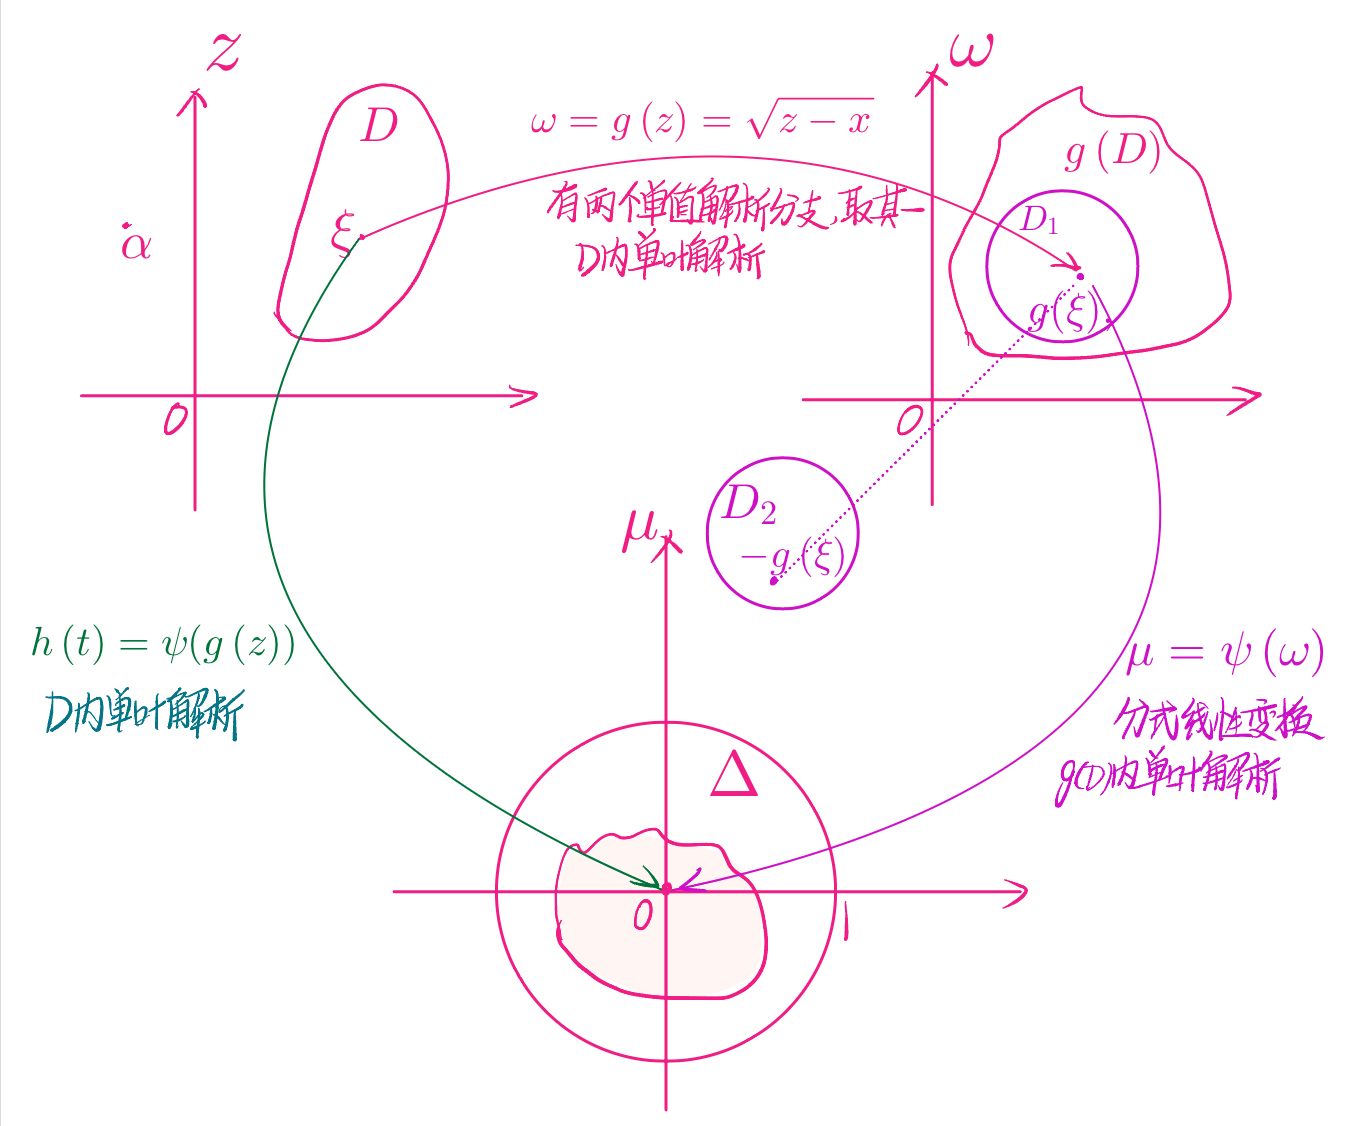
\includegraphics[width=.7\linewidth]{figures/IMG_6415.png}
    \caption{\textbf{Setp.I图示}}
    \label{fig:setpi}
\end{figure}
以 $g(\xi)$为圆心做一个包含在 $g(D)$内的圆盘 $D_1$,则 \textbf{\color{magenta!90!black}$D_1$关于原点对称的圆盘 $D_2$必然不会包含在 $g(D)$内}. 这是因为 $\forall\omega_1\in D_1,\exists z_1\in D$,使得 $g(z_1)=\omega_1$,假设 $-\omega_1\in g(D)$, 则 $\exists z_2\in D$,使得 $g(z_2)=-\omega_1$,即 $g(z_1)=-g(z_2), z_1,z_2\in D$, 与上述性质第二条矛盾. 

\textbf{\color{blue!50!black}构造 $\mu=\psi(\omega)$为分式线性变换,那么它\uwave{将 $g(\xi)$映为原点}, \uline{将 $g(D)$的内部映为单位圆盘的内}\newline\uline{部(不是整个单位圆盘)}.}
\begin{remark}
    \textbf{\color{red!50!black}$\mu$ 将圆盘 $D_2$的外部映成单位圆盘的内部}. 这总是可以做到的,\textbf{\color{red!50!black}只要保证两个圆盘的边界走向相反即可 (两个单位圆盘的边界走向一致时, $\mu$将 $\Delta$ 内部映成$\Delta$ 内部; 将$\Delta$ 外部映成$\Delta$ 外部; 两个单位圆盘的边界走向相反时, $\mu$将 $\Delta$ 外部映成$\Delta$ 内部; 将$\Delta$ 内部映成$\Delta$ 外部)}.
\end{remark}
将 $\mu=\psi(\omega)$和 $\omega=g(z)$复合后得到的函数 \uline{$h(z)=\psi(g(z))$在$D$内单叶解析},且
\[h(\xi)=\psi(g(\xi))=0.\]
但是 $h^\prime(\xi)$不一定大于零,所以不妨设 $h^\prime(\xi)=r\cdot e^{i\theta}$, 则 $e^{-i\theta}h^\prime(\xi)=r>0$.那么令 $\varphi(z)=e^{-i\theta}h(z)$,则 \uline{$\varphi^\prime(\xi)>0$},所以由上述划线部分知,$\varphi(z)$在 $D$内满足 $\mathscr{F}$的四个条件,从而 $\varphi\in\mathscr{F}$,则 $\mathscr{F}\neq \emptyset$.

由于 $g(D)$是圆盘 $D_2$外部的一部分,则由上述评注知, $g(D)$ 被 $\mu$ 映成单位圆盘内部的一部分. $\forall f\in\mathscr{F}, |f(z)|\leqslant 1$ 一致有界, 由 Montel定理知 $\mathscr{F}$是正规族.
\subsection{第二步: 证明 \texorpdfstring{$\sup_{f\in \mathscr{F}} f^\prime (\xi)$}.是有限数且它可在 \texorpdfstring{$D$}.内取到}\label{subsec:setp2}
补充结论: 上确界的一般性结论: $a=\sup S\implies \exists \{x_n\}\subset S$,使得 $\lim_{n\to\infty}x_n=a$.

设 $\sup_{f\in\mathscr{F}}f^\prime (\xi)=m\leqslant +\infty$ ($m>0$因 $f^\prime(\xi)>0$).则存在 $\{f_n\}\subset \mathscr{F}$,使得 $\lim_{n\to\infty}f^\prime_n (\xi)=m$.
因 $\mathscr{F}$是正规族,故
\begin{eq}\label{eq:1.1.1}
    \exists \{f_{n_k}\}\subset \{f_n\}\text{使得} f_{n_k}\overset{d}{\to}f\overset{(a)}{\implies} f^\prime_{n_k}\to f^\prime \overset{(b)}{\implies} \lim_{k\to\infty}f^\prime_{n_k}(\xi)=f^\prime(\xi).
\end{eq}
其中 $(a)$是因为\textbf{\color{red}原函数列内闭一致收敛那么导函数列也必内闭一致收敛 (由Cauchy积分公式证明)}; $d$表示内闭一致收敛; $(b)$为定义.
\begin{eq}
\label{eq:1.1.2}
    \text{因} \lim_{n\to\infty}f^\prime_n (\xi)=m, \text{则} \lim_{k\to\infty}f_{n_k}^\prime (\xi)=m.
\end{eq}
因此, 结合\textbf{\eqref{eq:1.1.1}}、\textbf{\eqref{eq:1.1.2}}可得 $f^\prime(\xi)=m$. 又由$\mathscr{F}$的定义知, $f^\prime(\xi)=m>0$.

因为 $f$为单叶解析函数列内闭一致收敛的极限函数,由 定理, $f$要么是单叶解析函数, 要么是常数,但由于 $f^\prime(\xi)>0$,故 $f$不能是常数,所以 $f$是单叶函数, $m=f^\prime(\xi)<+\infty$.
注意到,
\begin{eq}
    f(\xi) &=\lim_{k\to\infty}f_{n_k}(\xi)=0 ,\\ 
    |f(z)| &=\left|\lim_{k\to\infty}f_{n_k}(z)\right|\overset{(c)}{=}\lim_{k\to\infty}\left|f_{n_k}(z)\right|\overset{(d)}{\leqslant} 1.
\end{eq}
其中, $(c)$表示取模运算与极限运算次序可交换,因为取模运算是连续的; $(d)$表示极限只能保非严格不等式.下面排除 $|f(z)|=1$的情形. (反证法) 若 $|f(z)|=1$, 注意到 \textbf{模(实部)(虚部)(辐角)为常数的解析函数必为常数},则 $f$为常数,矛盾,因而 $|f(z)|<1$.
故 $f\in\mathscr{F}$,且 $f$是 $\mathscr{F}$中导数取得最大值的那一个.
\subsection{第三步: 证明上面找到的 \texorpdfstring{$f$}.即要找的映满共形映射 \texorpdfstring{$f(D)=\{\omega\colon |\omega|<1\}$}.}\label{subsec:setp3}
\begin{figure}[htb]
    \centering
    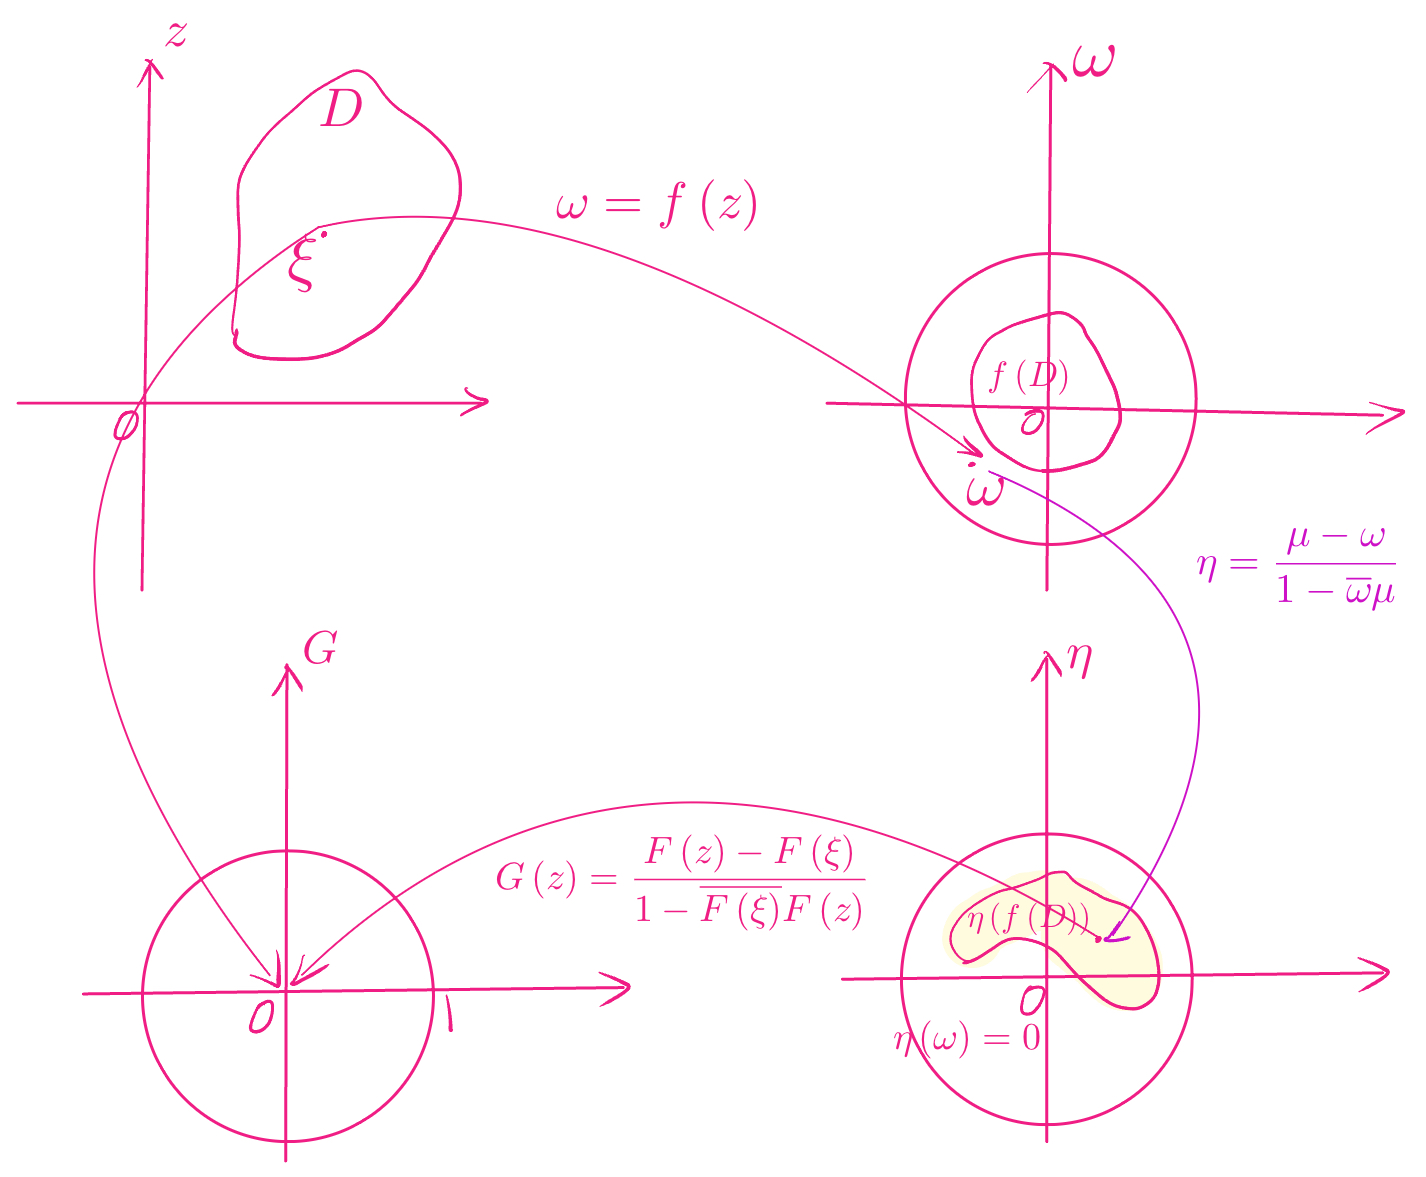
\includegraphics[width=.7\linewidth]{figures/IMG_6416.png}
    \caption{Step.III 图示}
    \label{fig:setpiii}
\end{figure}
(反证法) 设 $f(D)\neq \Delta$,即存在 $\omega\in\Delta\backslash f(D)$,取之构成分式线性变换 
\begin{eq}
    \label{eq:eta}
    \eta=\frac{f(z)-\omega}{1-\overline{\omega}f(z)}=\frac{\mu-\omega}{1-\mu\omega},
\end{eq}
则\textbf{\color{magenta}该分式线性变换将 $\omega$平面单位圆盘内的区域映成 $\eta$平面单位圆盘内的区域 (不含原点,因 $\eta(\omega)=0$, 但$\omega\not\in f(D)$)}.

设 
\begin{eq}
    \label{eq:F}
    F(z)=\sqrt{\frac{f(z)-\omega}{1-\overline{\omega}f(z)}},
\end{eq}
我们断言, $F(z)$在 $D$内单叶解析.
因 $F(z)$在 $D$内无零点,由引理可知, $F(z)$在 $D$内有单值解析分支,不妨取其一表为 $F(z)$. 若 $F(z_1)=F(z_2)$,则
\begin{eq}
    \label{eq:1.1.4}
    \frac{f(z_1)-\omega}{1-\overline{\omega}f(z_1)}=\frac{f(z_2)-\omega}{1-\overline{\omega}f(z_2)}\implies f(z_1)=f(z_2)\overset{f\text{单叶解析}}{\implies} z_1=z_2.
\end{eq}
故 \uline{$F(z)$在 $D$内是单叶解析的.}
且 \uline{\color{magenta}$|F(z)|<1$}.但这不足以使 $F(z)\in\mathscr{F}$,这是因为 $F(\xi)\not\equiv 0$.(经分式线性变换$\eta$作用后的像区域不含原点)
为此, 我们再做一次复合, 使得 
\begin{eq}
    \label{eq:G}
    G(z)=e^{-i\theta}\cdot \frac{F(z)-F(\xi)}{1-\overline{F(\xi)}F(z)},\text{其中} e^{-i\theta}=\frac{F^\prime (\xi)}{|F^\prime(\xi)|},
\end{eq}
这是因为由 \textbf{\ref{subsec:setp1}} 知 
\begin{eq*}
    e^{-i\theta}=\frac{h^\prime(\xi)}{|h^\prime(\xi)|}=\frac{F^\prime (\xi)}{|F^\prime(\xi)|}
\end{eq*}
($h$到 $F$只做了一次分式线性变换而没有旋转,因而不改变辐角).这样即可得到 $G(\xi)=0$,且 $G^\prime (\xi)>0$ ; 又$G$在 $F$基础上做旋转, 不改变模长, $|G(z)|=|F(z)|<1$ ($G$将 $F(\xi)$变为原点; ).故 $G(z)\in \mathscr{F}$.

又由于
\begin{eq}
    \label{eq:1.1.5}
    G^\prime(\xi)=\frac{|F^\prime (\xi)|}{1-|F(\xi)|^2}=\frac{1+|\omega|}{2\sqrt{\omega}}f^\prime(\xi)>f^\prime (\xi).
\end{eq}
这与\textbf{\ref{subsec:setp2}}的结论: $f^\prime(\xi)$是 $\mathscr{F}$中导数最大者矛盾,故
$G(z)$即为我们要找的映满的共形映射.

\end{proof}




















\normalem
\printbibliography[
heading=bibintoc,
title={参考文献}
]
\printindex
\summary{本书是复分析学的结课期考复习资料总结,主要包括了考试的证明题型以及各类的识记知识点,如黎曼映射定理、广义Schwarz引理等等。本书由本人期末写成, 仅用于复习.}
\makebottomcover
\end{document}